\cleardoublepage%
\chapter{\label{chap:methods}Methodology}%

The research in this thesis can be divided into three distinct phases, Section \ref{sec:methods_ph1} Phase 1 consists of the analysis of the Smart Motor system, the literature and technology review, and the design of the networking and platform architecture, including a framework and guiding principles. Section \ref{sec:methods_ph2} Phase 2 describes the development of the networking and the supporting Smart System Platform, including some of its key features such as the GitHub page, the website, and various development and management tools. Section \ref{sec:methods_ph3} Phase 3 outlines the methodology for testing, validating and deploying the designed platform and networking capabilities.

\section{\label{sec:methods_ph1}Phase 1: Analysis and Design}

The first step, detailed in Section \ref{sec:methods_sm_analysis}, was to dissect and analyse the existing Smart Motor project, its system design and the technology used. In Section \ref{sec:methods_tech_review} all components of the Smart Motor v3 are examined. 
In this section, other systems and technologies are also examined, particularly with regard to networking solutions, focusing on, but not limited to, the components examined as part of the Smart Motors. 
Based on this analysis, a network design concept was developed, which is described in Section \ref{sec:methods_net_des}. Furthermore, based on considerations of how to support and provide accessibility to the system and its networking capabilities, a concept for an overarching system architecture, including supporting tools, development whatnot, was designed and is presented in Section \ref{sec:methods_ssp_des}.
%Iterative development of both the platform and the other stuff, make it future ready

\subsection{\label{sec:methods_sm_analysis}Smart Motor Technology Analysis and Review}

As defined by \citet[]{dahal_designing_2024}, the main components of the Smart Motor concept and how they interact are shown in Figure \ref{fig:sm_schematic} and consist of the MC as the brain of the system in its centre, a sensor input, a motor output and a user interface (UI) that provides both input and output and enables user-system interaction.

\begin{figure}[H]
    \centering
    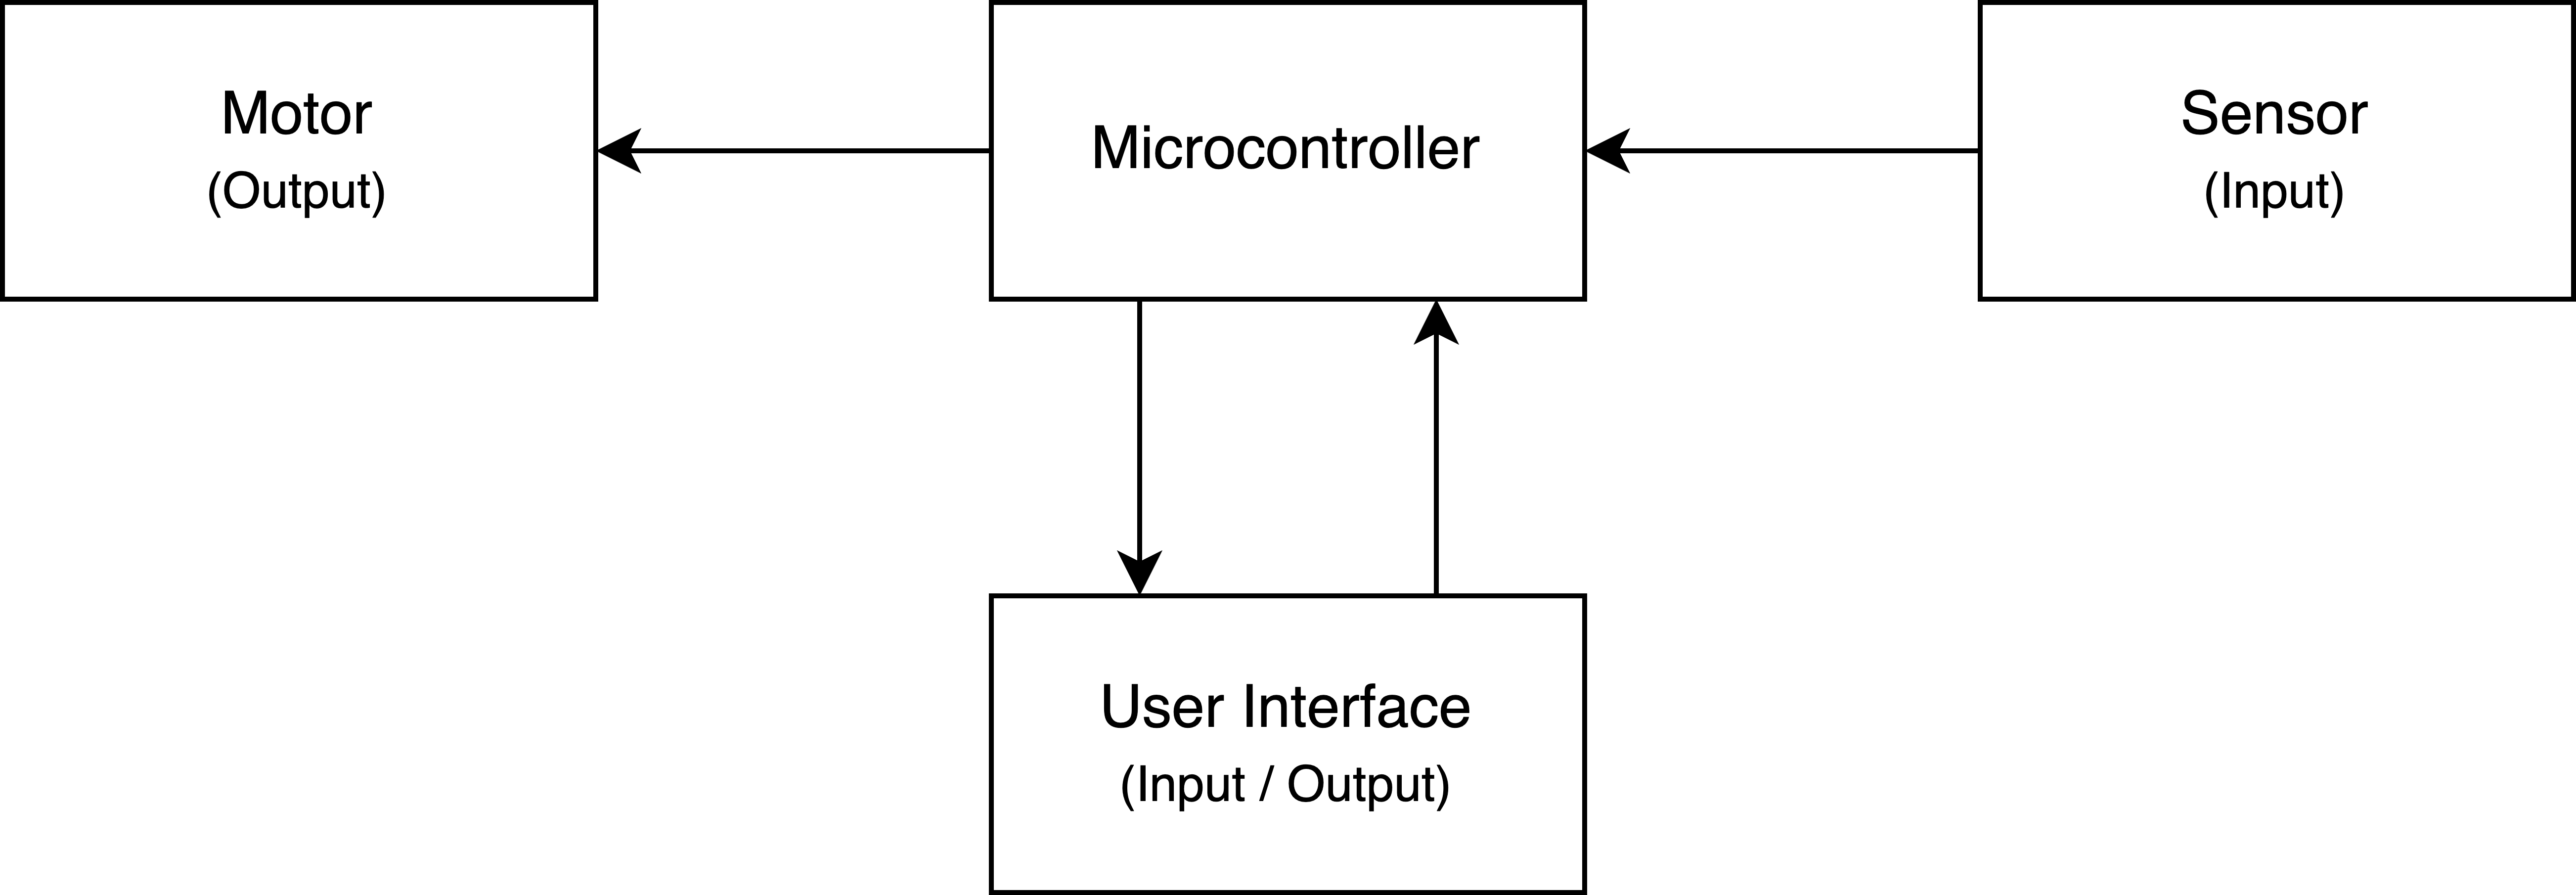
\includegraphics[width=0.75\linewidth]{overleaf/images/sm_concept.png}
    \vspace{\ftspace}
    \caption{General schematic of a Smart Motor system, adapted from \citet[p. 19]{dahal_designing_2024}}
    \label{fig:sm_schematic}
\end{figure}

There are two different modes of operation, \textit{Training} and \textit{Playing}. In the training mode, the user matches a given sensor input $S_n$ to a manually set motor output (either position or speed) $P_n$ using the UI, where $n$ is the index of the input data pair.
In play mode, the motor determines the output of the motor $P_{output}$ based on the current sensor input $S_{current}$ using a simplified nearest-neighbour algorithm described in Equation \ref{ml_nn_eq} with the machine learning (ML) training data provided by the user during the training mode, if $n \geq 1$.

\begin{equation}\label{ml_nn_eq}
    P_{\text{output}} = P_{arg\ min_{x \in {1,\ldots,n}} |S_{\text{current}} - S_x|}
\end{equation}

The simple algorithm compares the current sensor input $S_{current}$ with all $n$ stored sensor inputs $S_n$ from training and solves for which $S_x$ the Euclidean distance $|S_{current}-S_x|$ is minimal. As motor output $P_n$ and sensor input $S_n$ are always entered in pairs and therefore linked, the motor output $P_x$ is linked to the sensor input $S_x$ and is then used to set the output of the motor accordingly.
\\\\
This section focuses on the design, technology and function of the Smart Motor, with particular emphasis on the latest iteration of the Smart Motor, the Smart Motor v3 \citep[p. 38]{dahal_designing_2024}.

\subsubsection{\label{sec:methods_sm_mech}Hardware Design}

Physically, the Smart Motor v3 is cube-shaped, with its various components contained within the shell, with only the various physical interfaces visible on the surface. 
An OLED screen, a button and a potentiometer are located on the front face. There are two more buttons on the left, a Grove-compatible sensor port on the right, and a USB-C port on the bottom. The motor, either a servo or a continuous motor, extrudes on the top. The shell is a mix of 3D printed and laser-cut parts, with the newer version being fully 3D printed. Contained within the shell is a lithium polymer battery.

\begin{figure}[H]
    \centering
    \begin{subfigure}[b]{0.25\textwidth}
        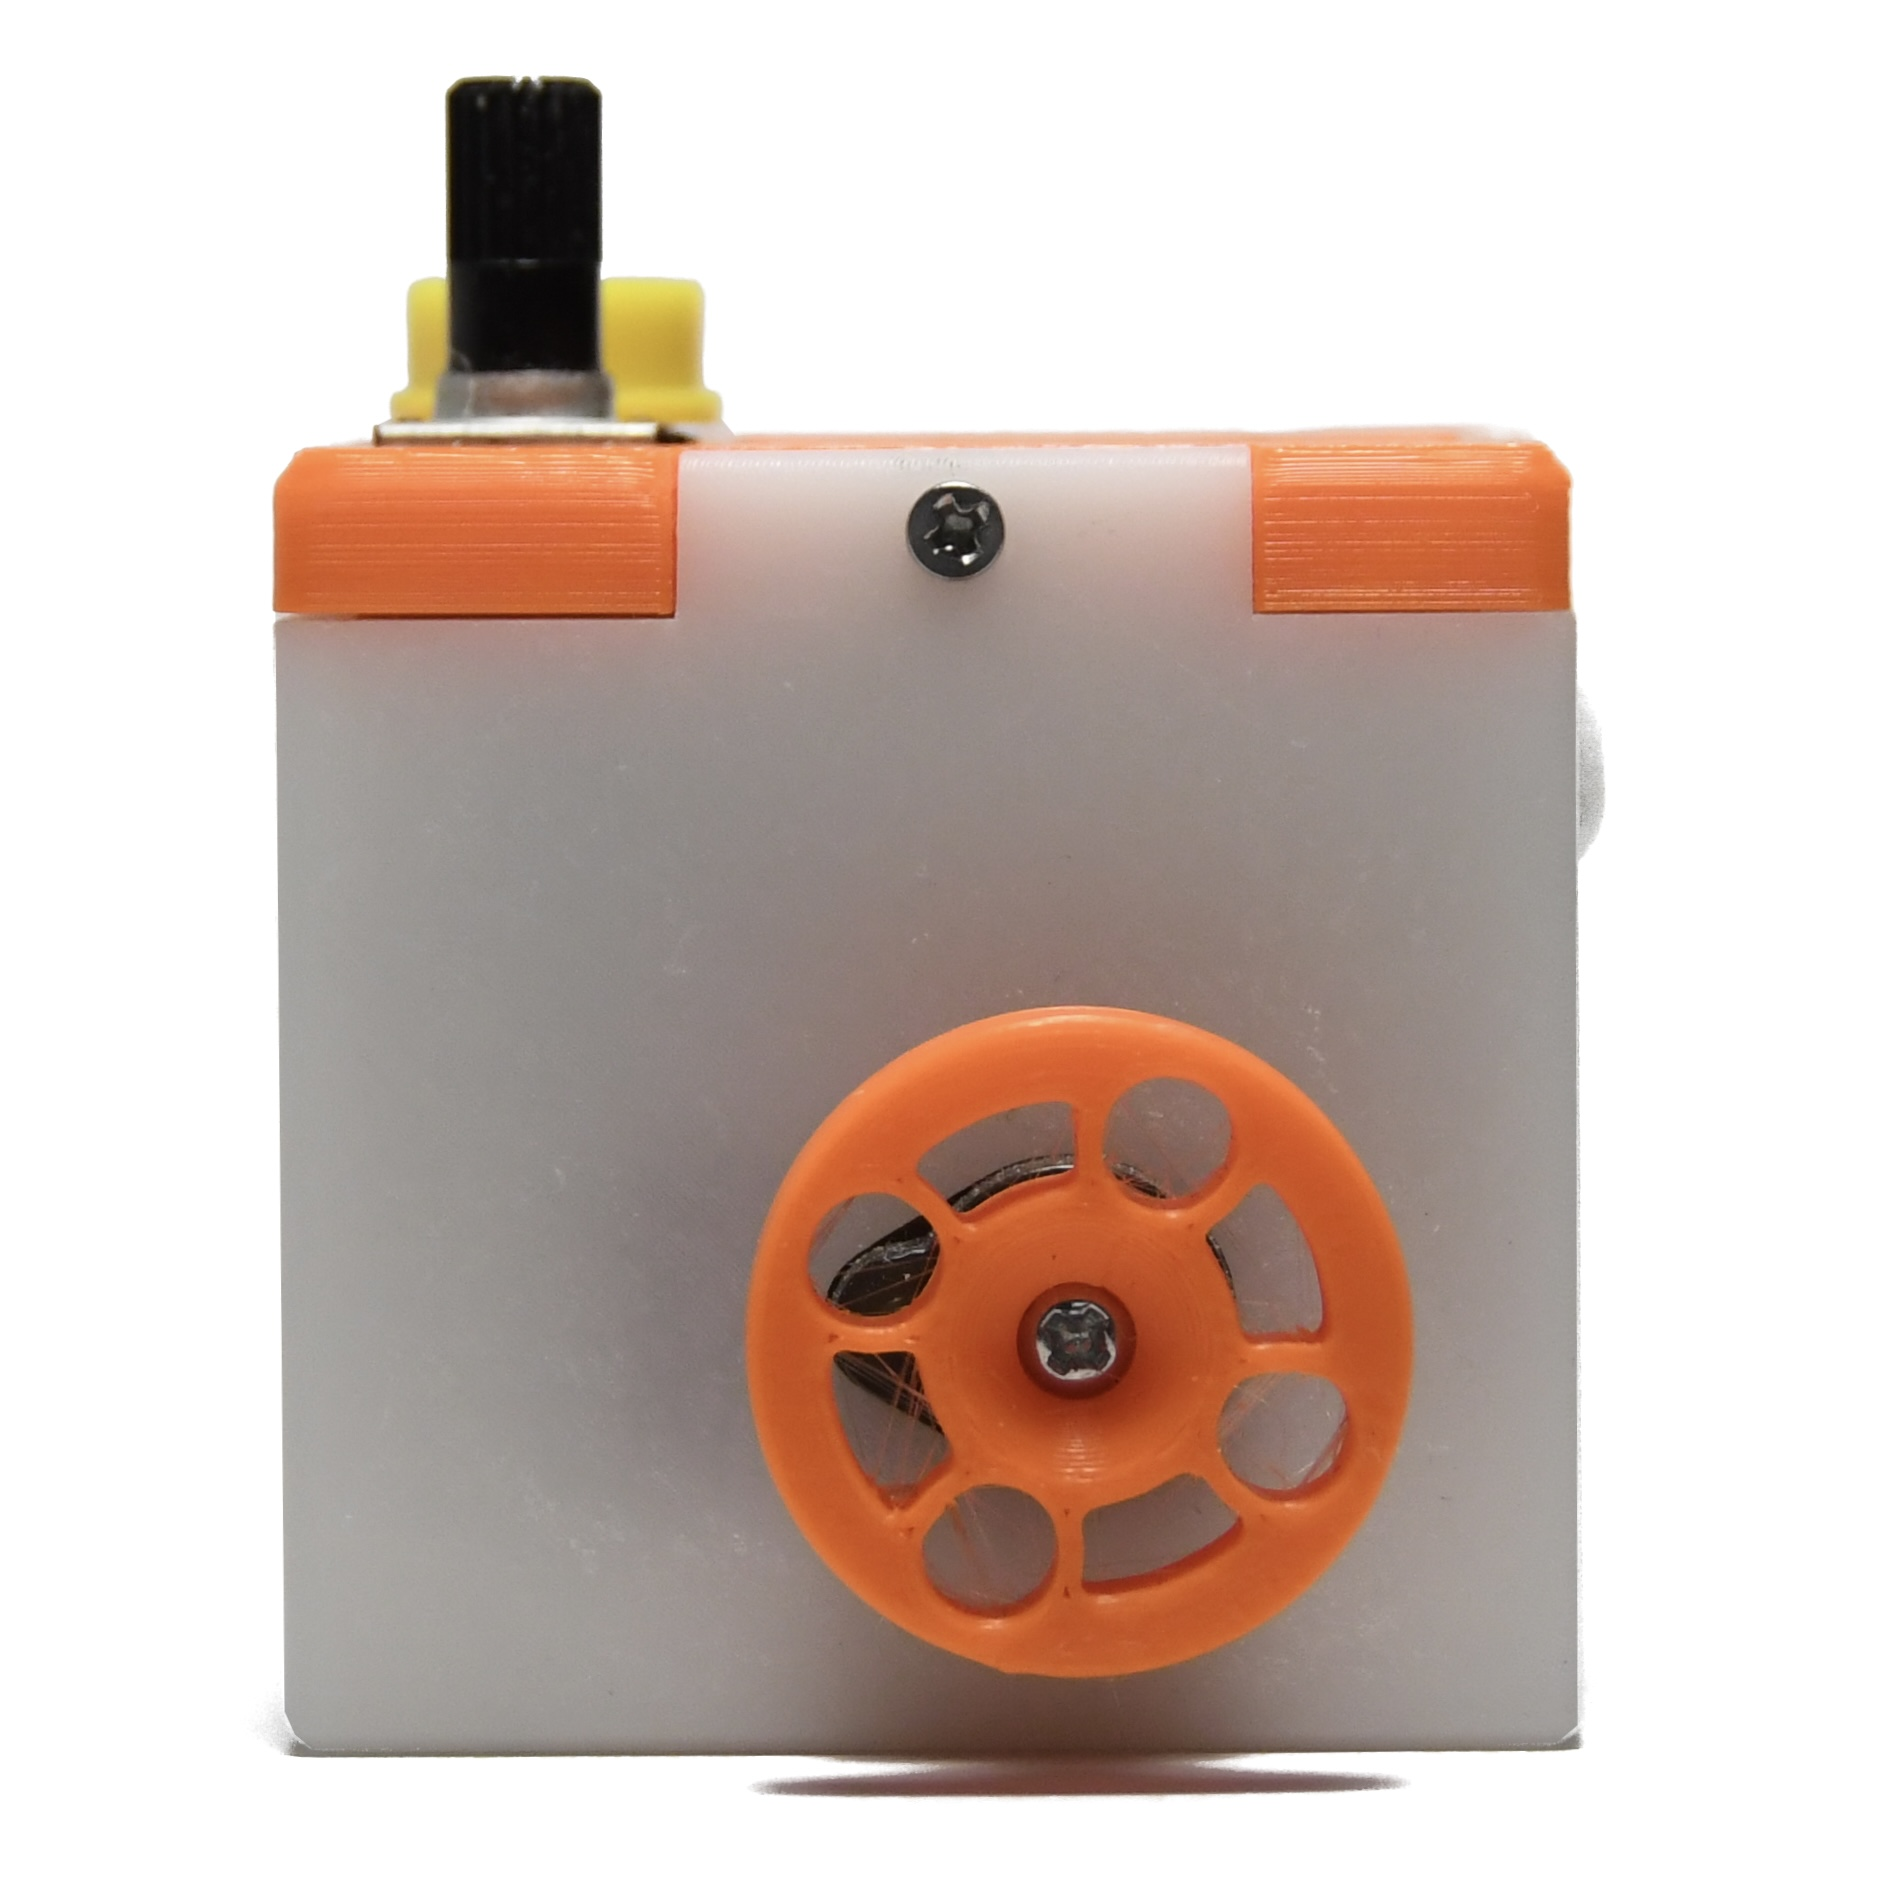
\includegraphics[width=\linewidth]{overleaf/images/sm_top.jpg}
    \end{subfigure}
    \begin{subfigure}[b]{0.25\textwidth}
        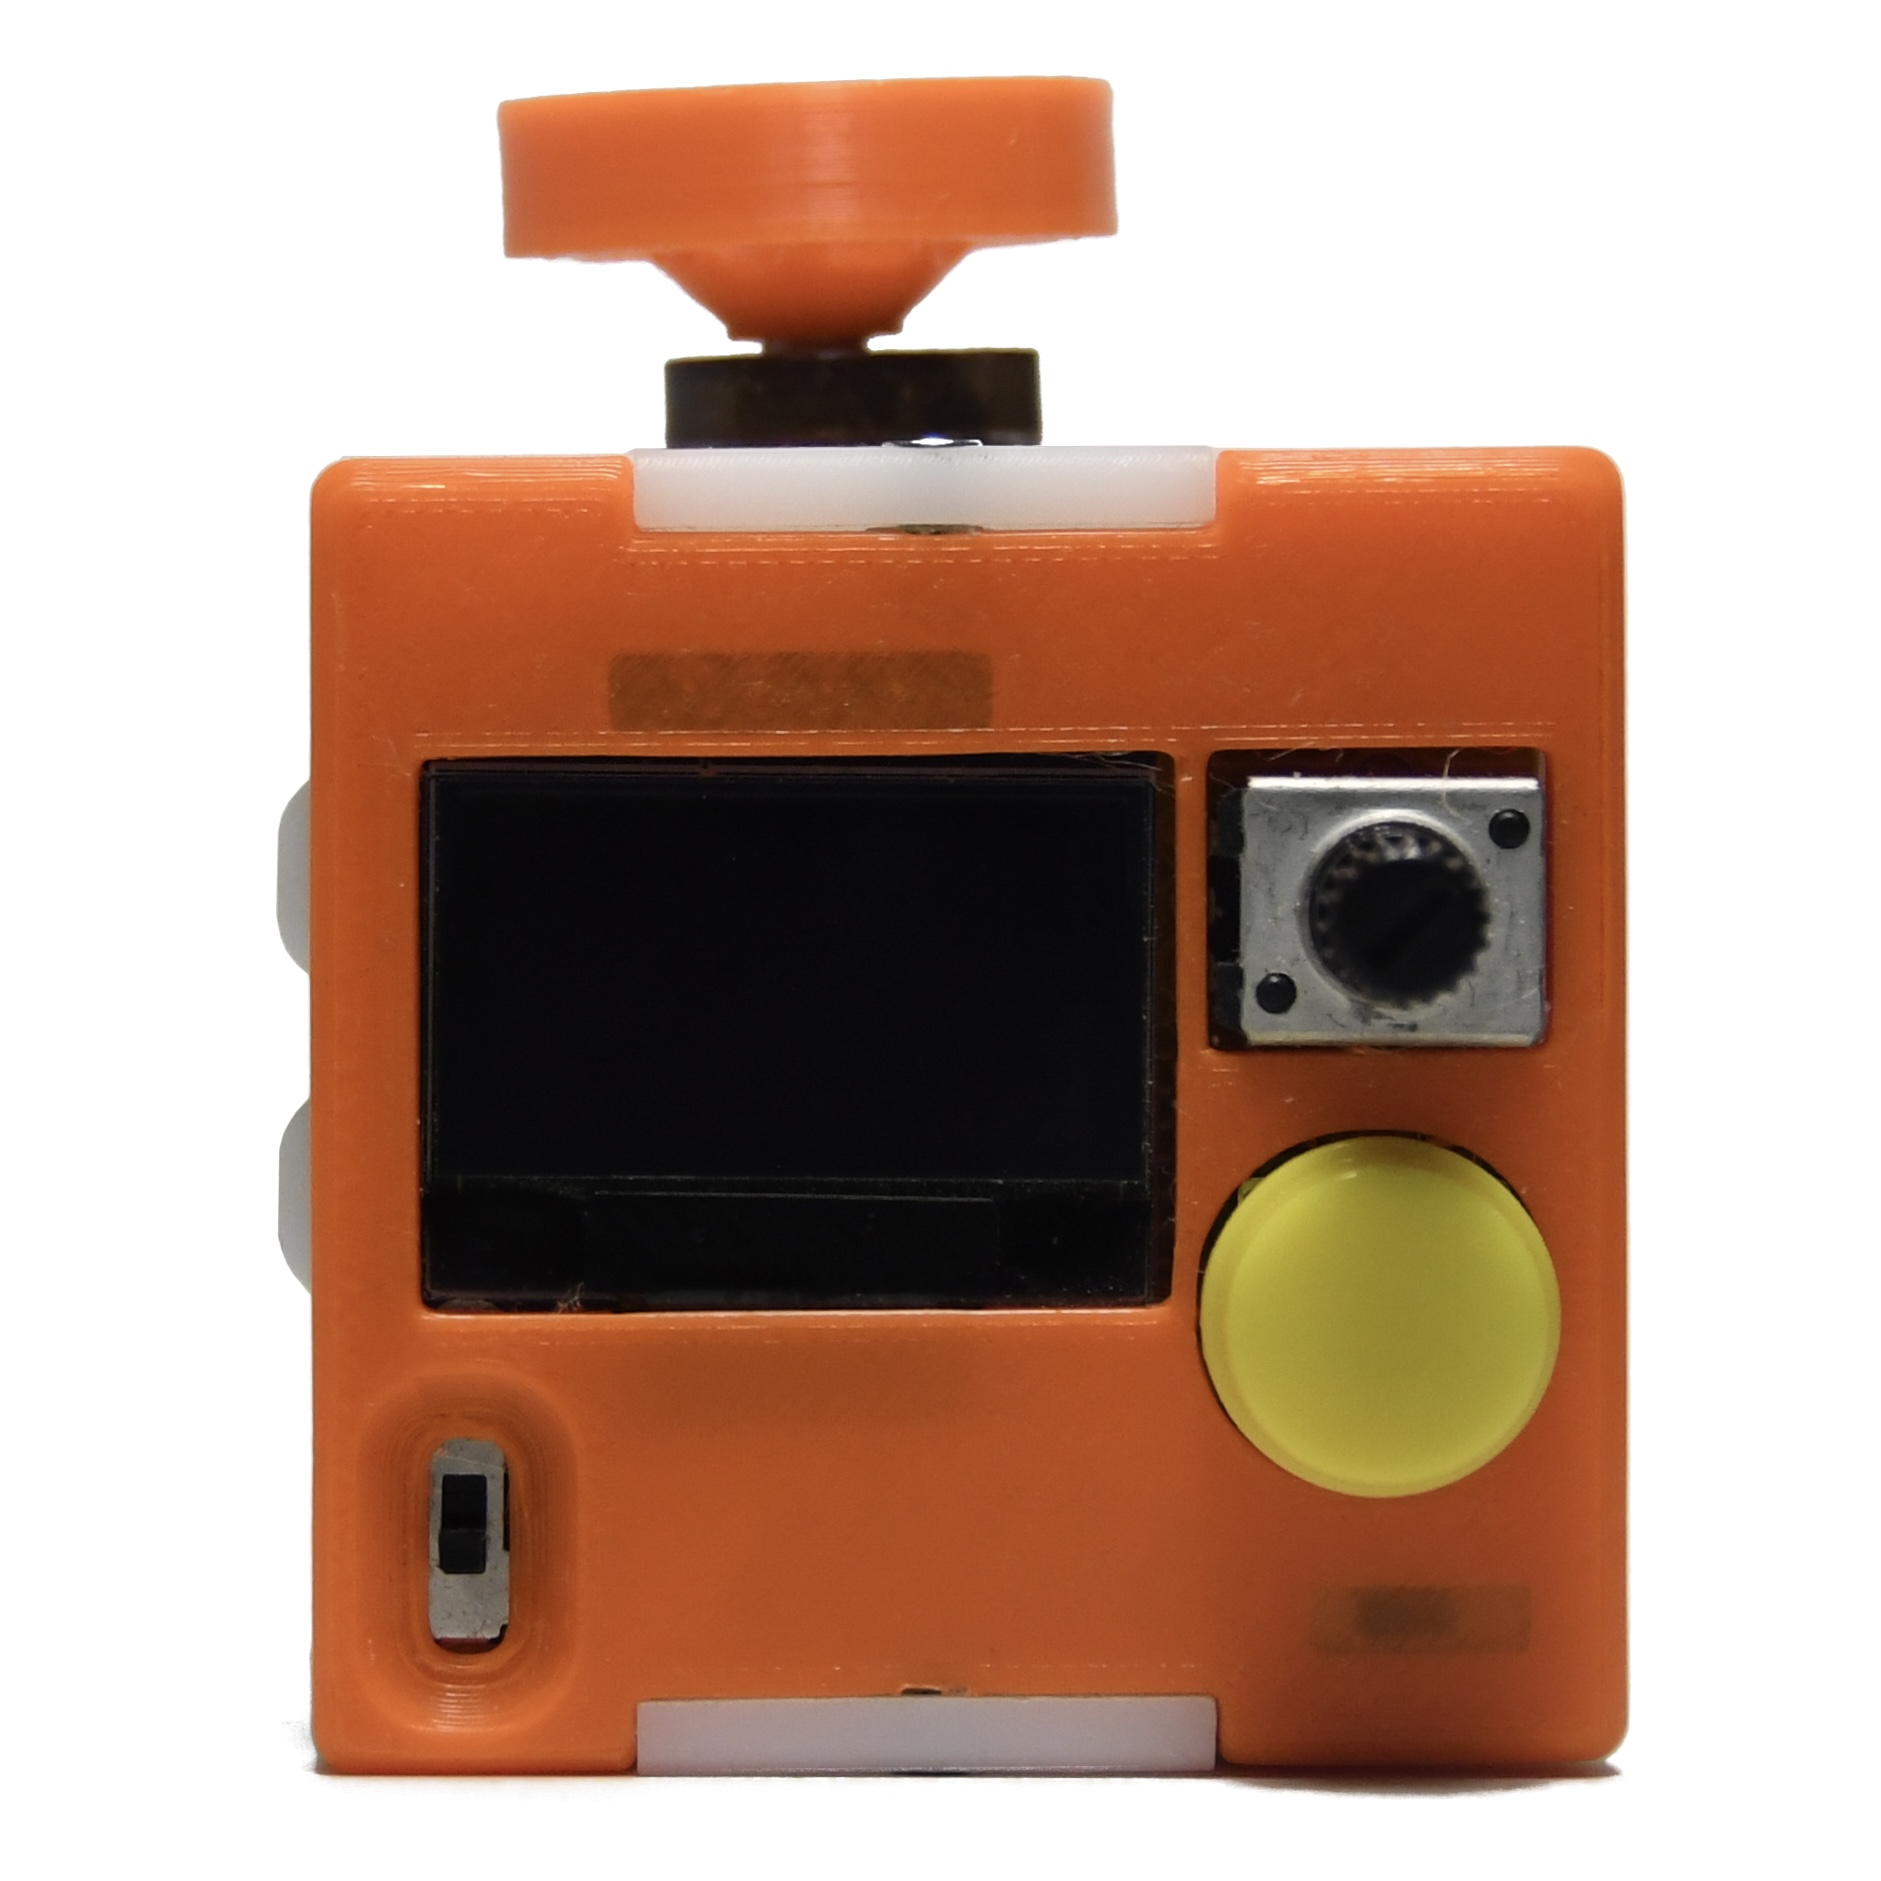
\includegraphics[width=\linewidth]{overleaf/images/sm_front.jpg}
    \end{subfigure}
    \begin{subfigure}[b]{0.25\textwidth}
        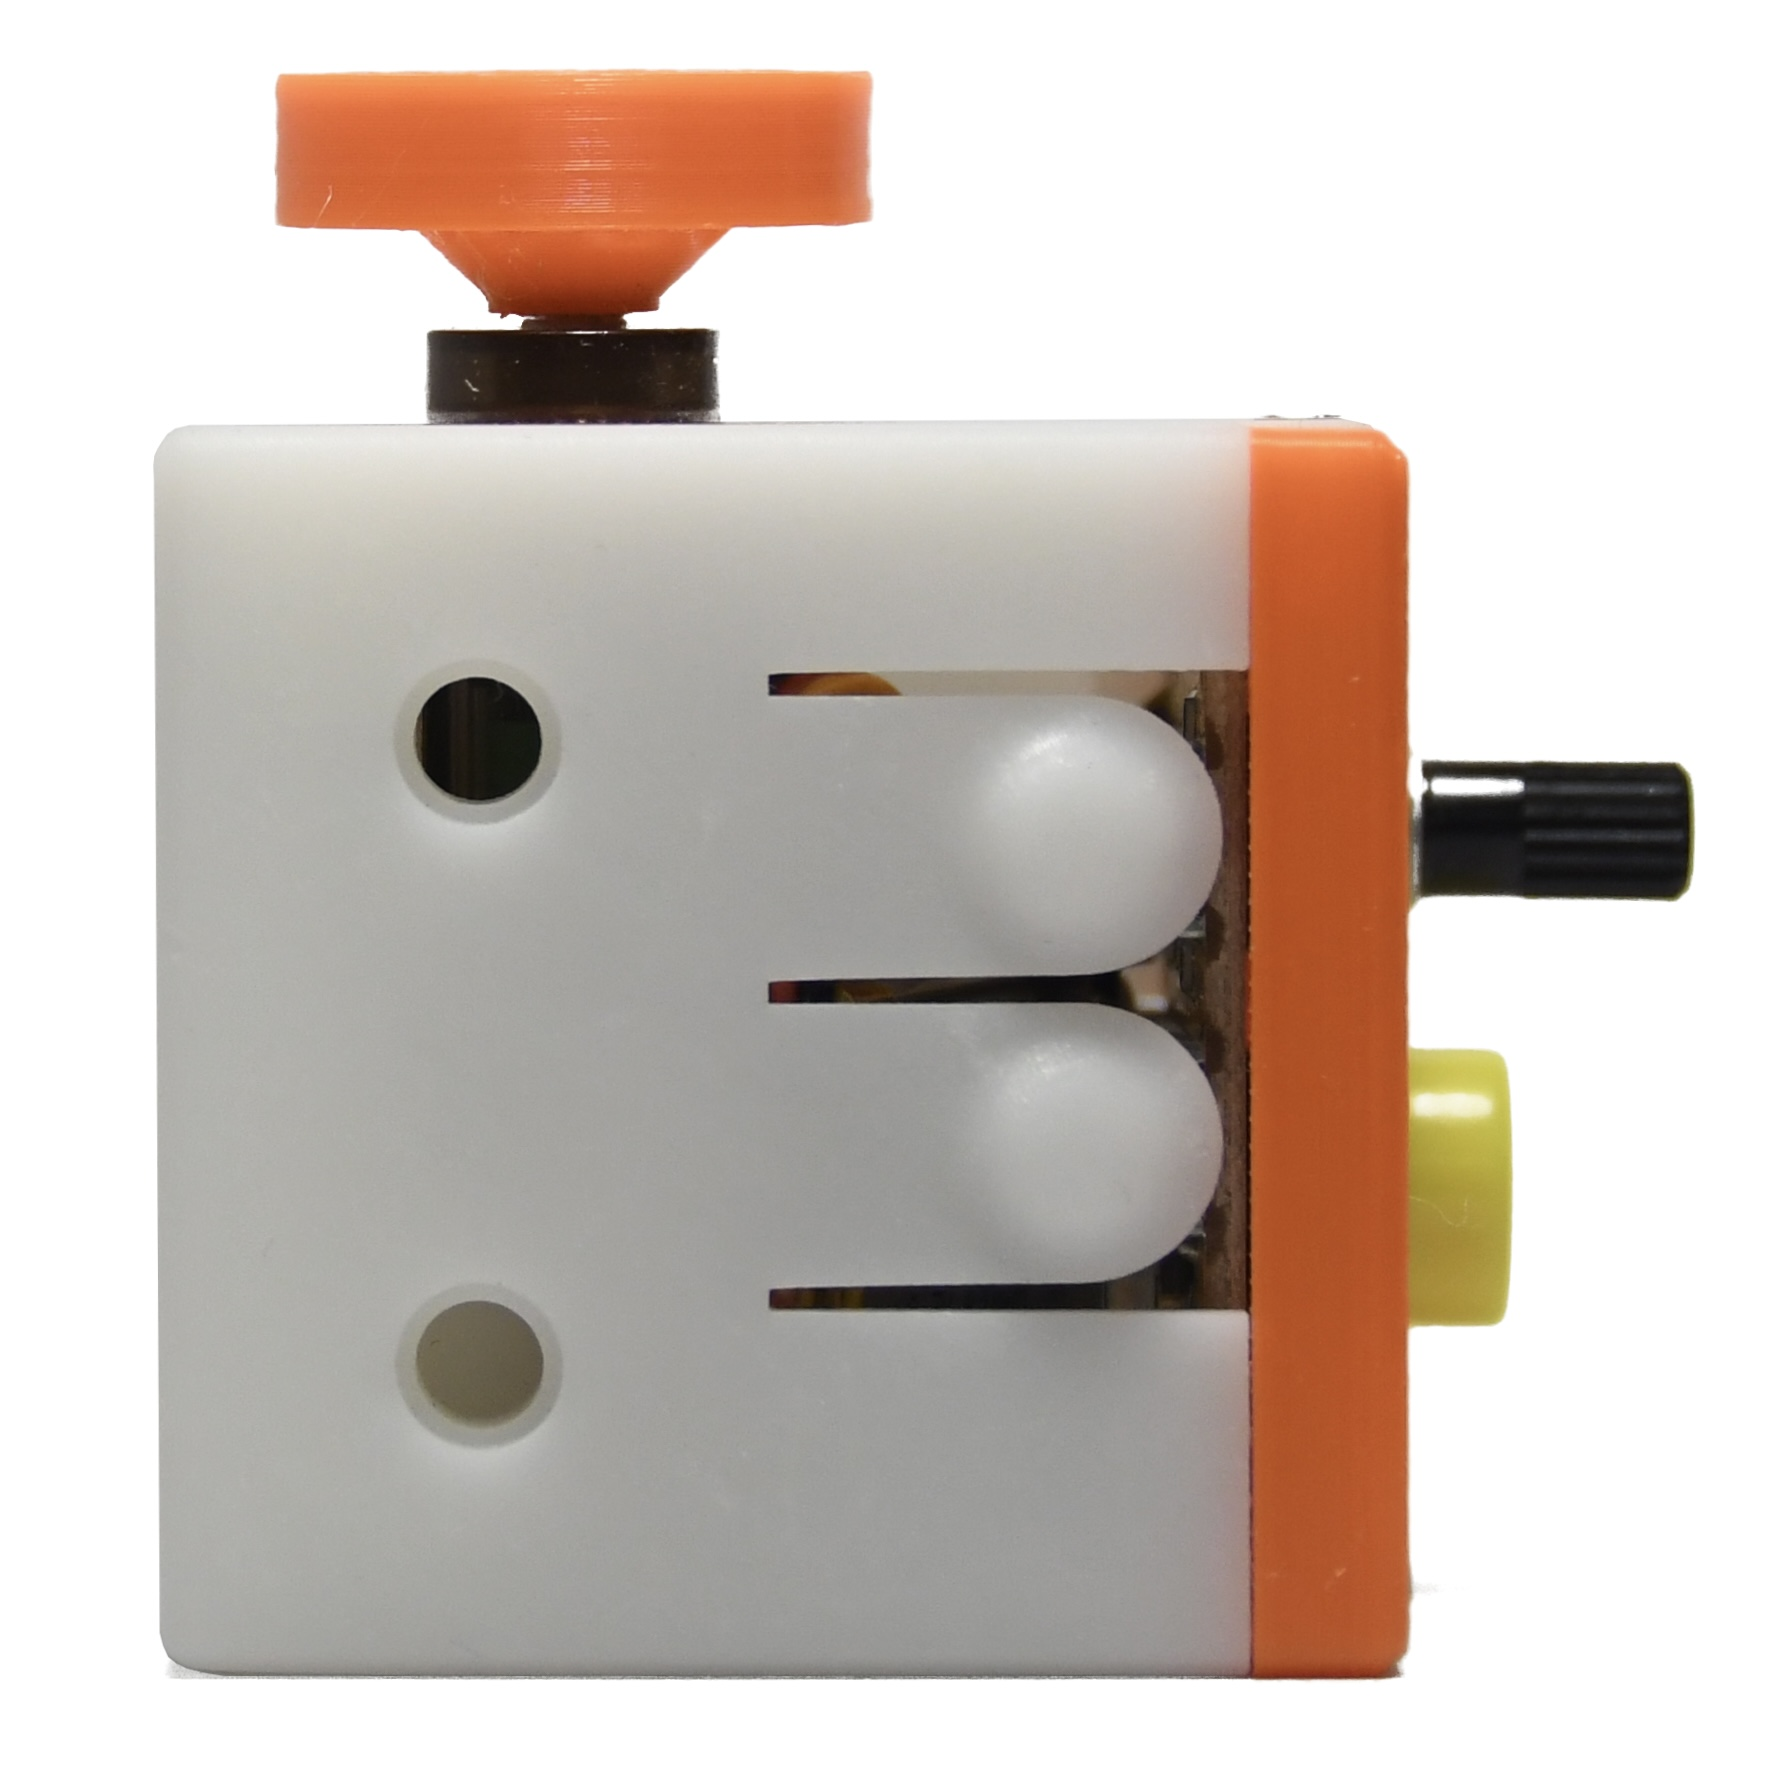
\includegraphics[width=\linewidth]{overleaf/images/sm_left.jpg}
    \end{subfigure}
    \\\vspace{2pt}
    \begin{subfigure}[b]{0.25\textwidth}
        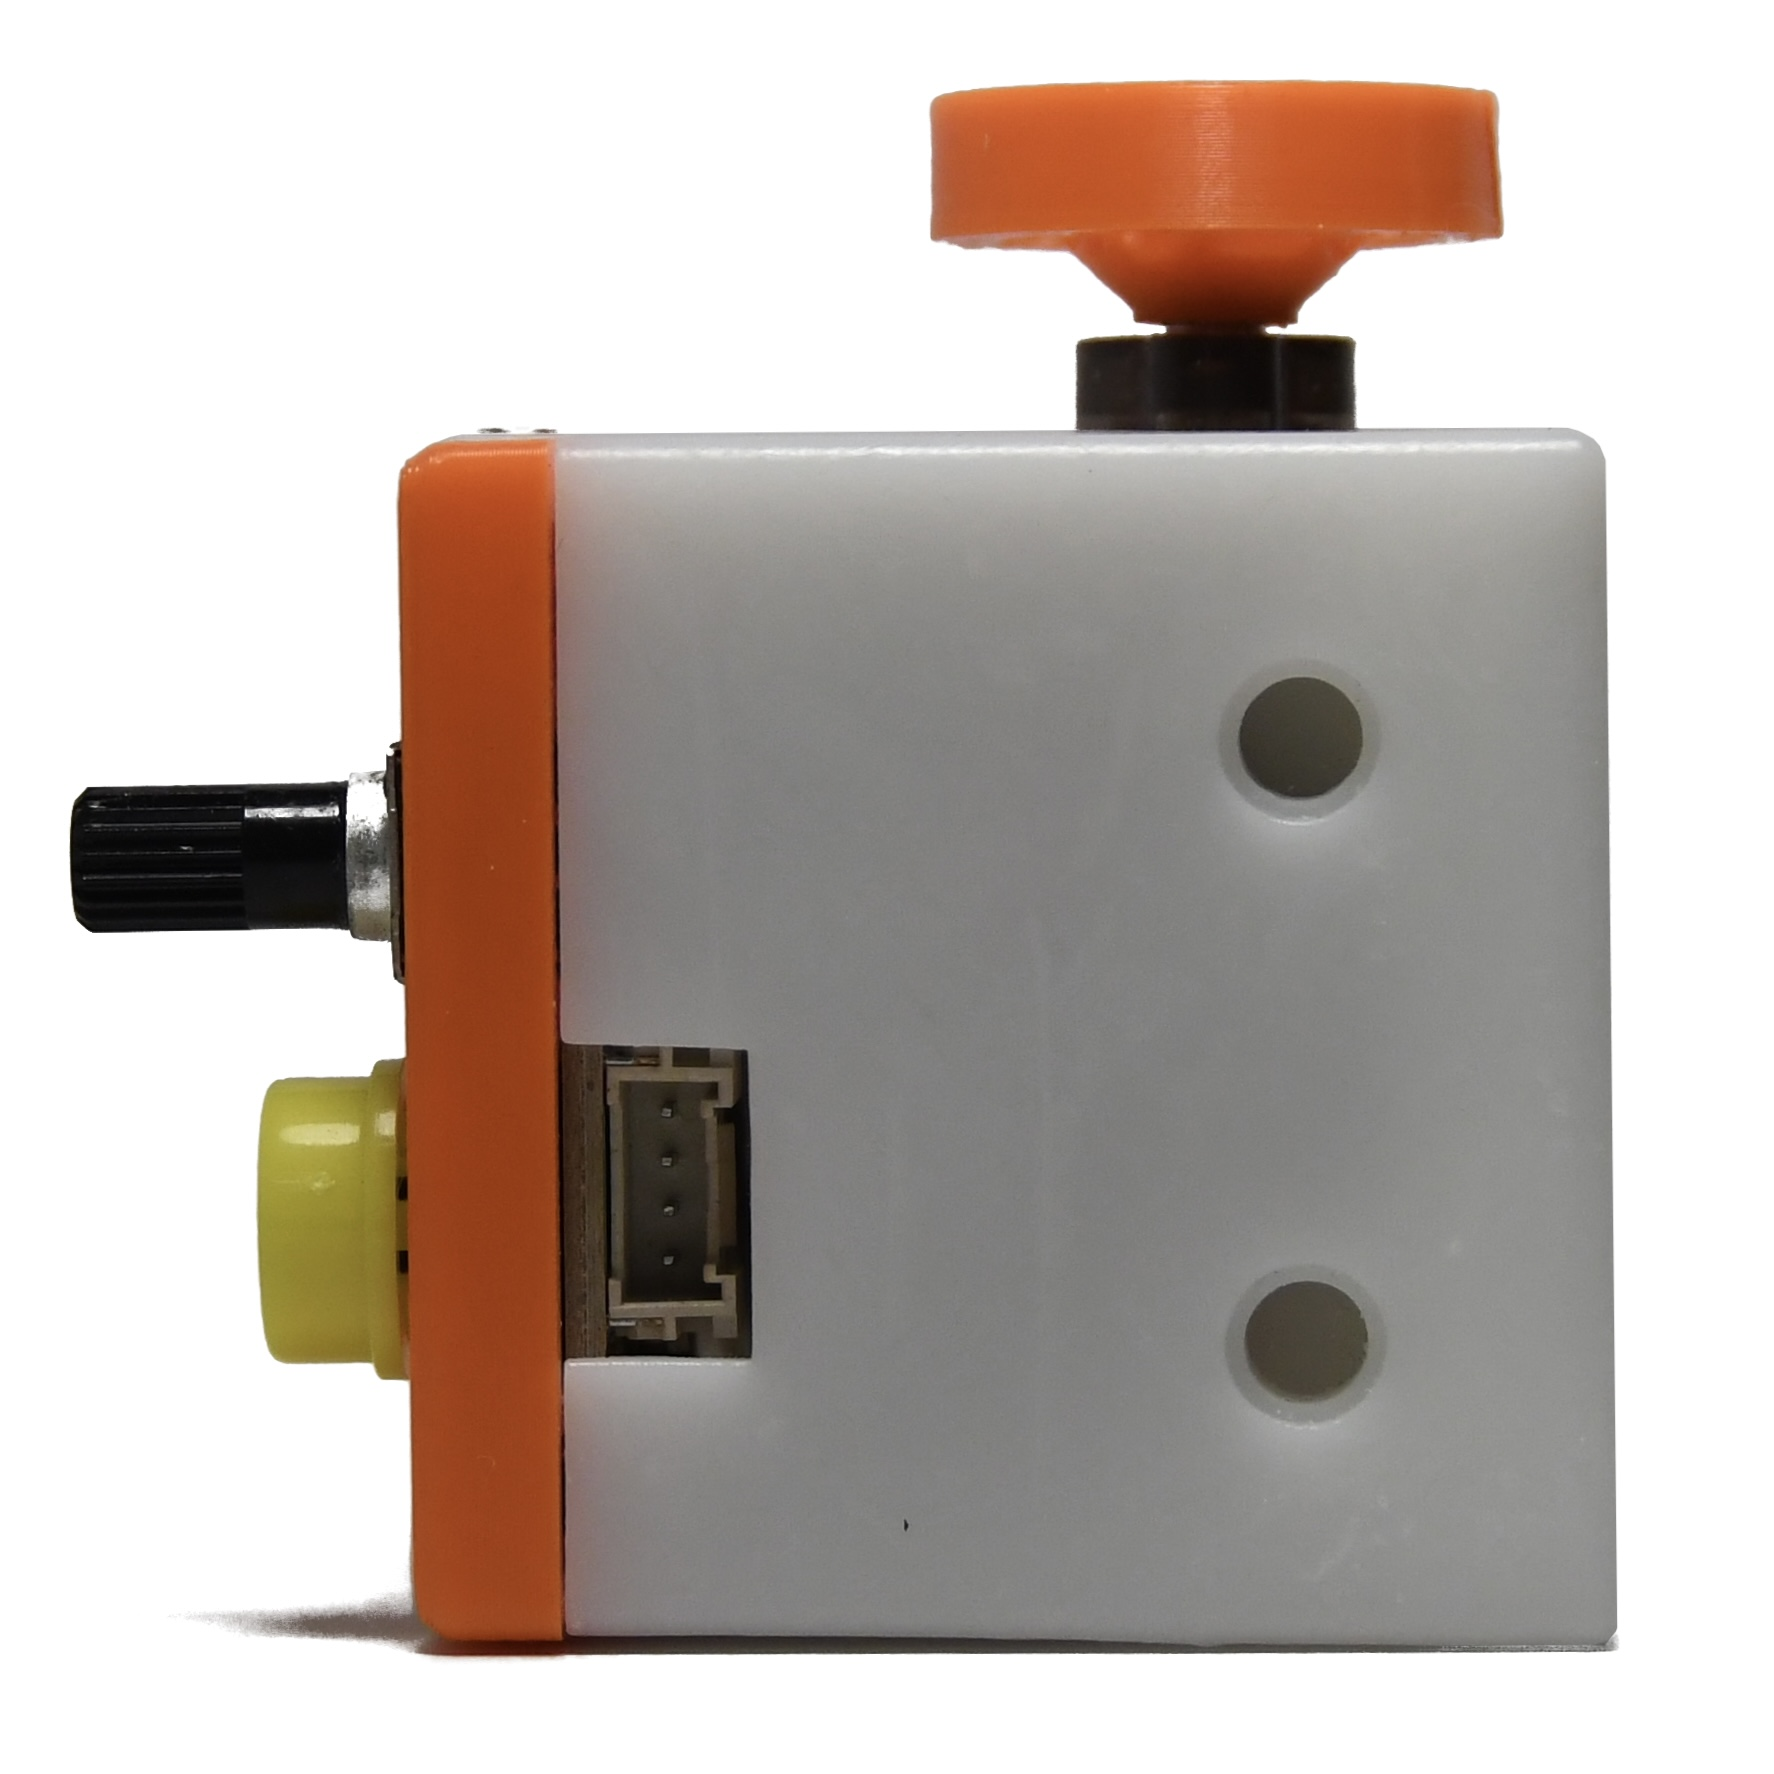
\includegraphics[width=\linewidth]{overleaf/images/sm_right.jpg}
    \end{subfigure}
    \begin{subfigure}[b]{0.25\textwidth}
        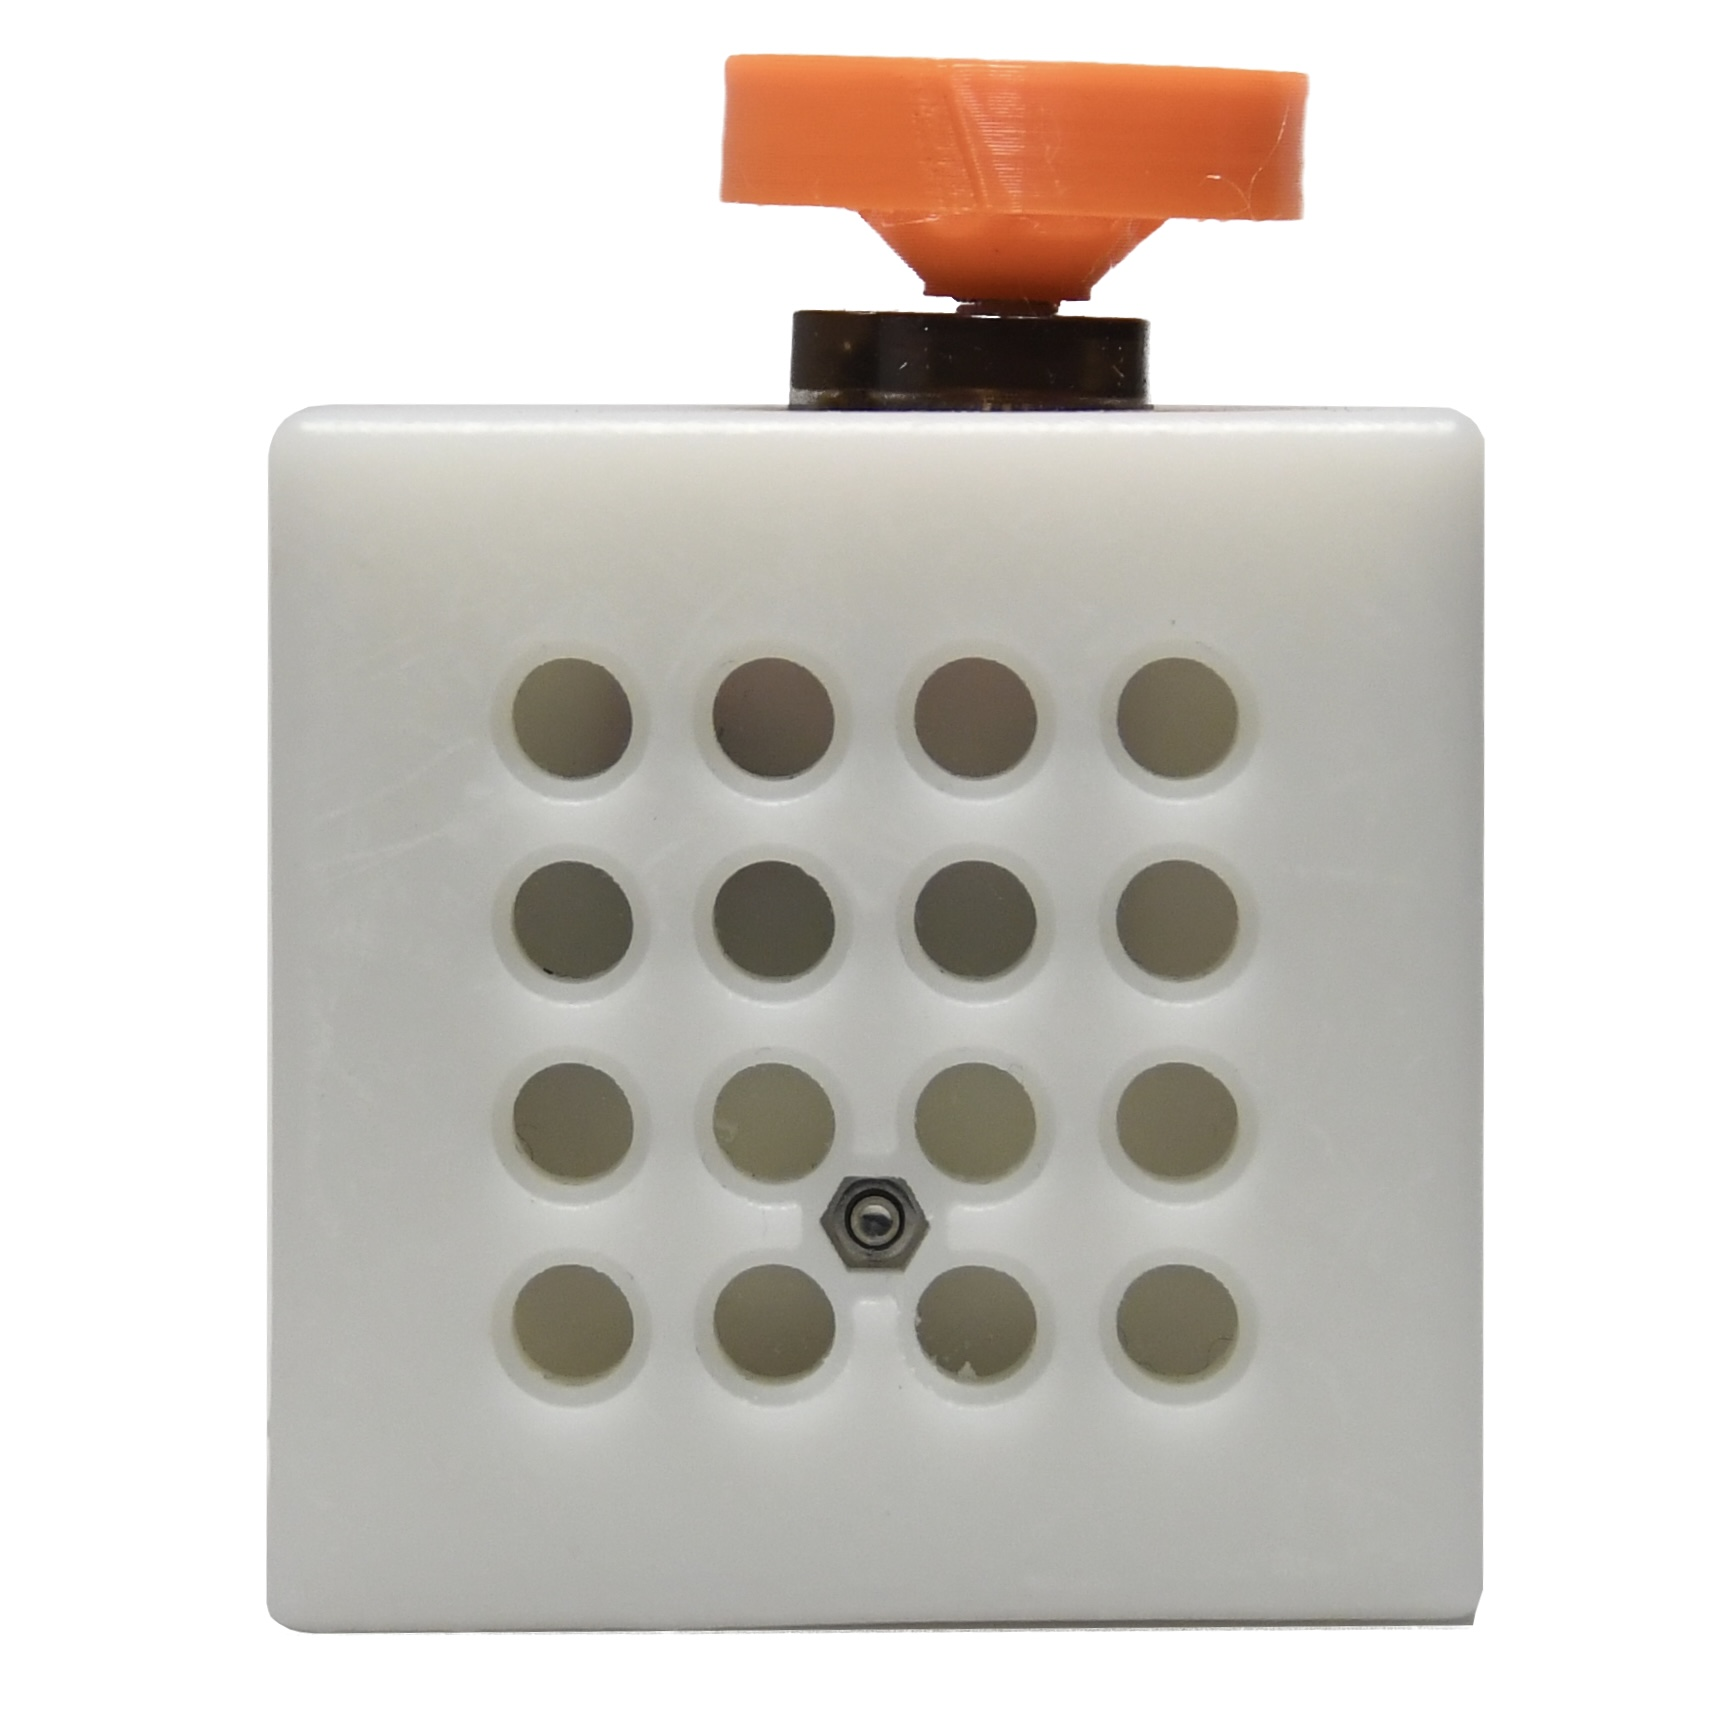
\includegraphics[width=\linewidth]{overleaf/images/sm_back.jpg}
    \end{subfigure}
    \begin{subfigure}[b]{0.25\textwidth}
        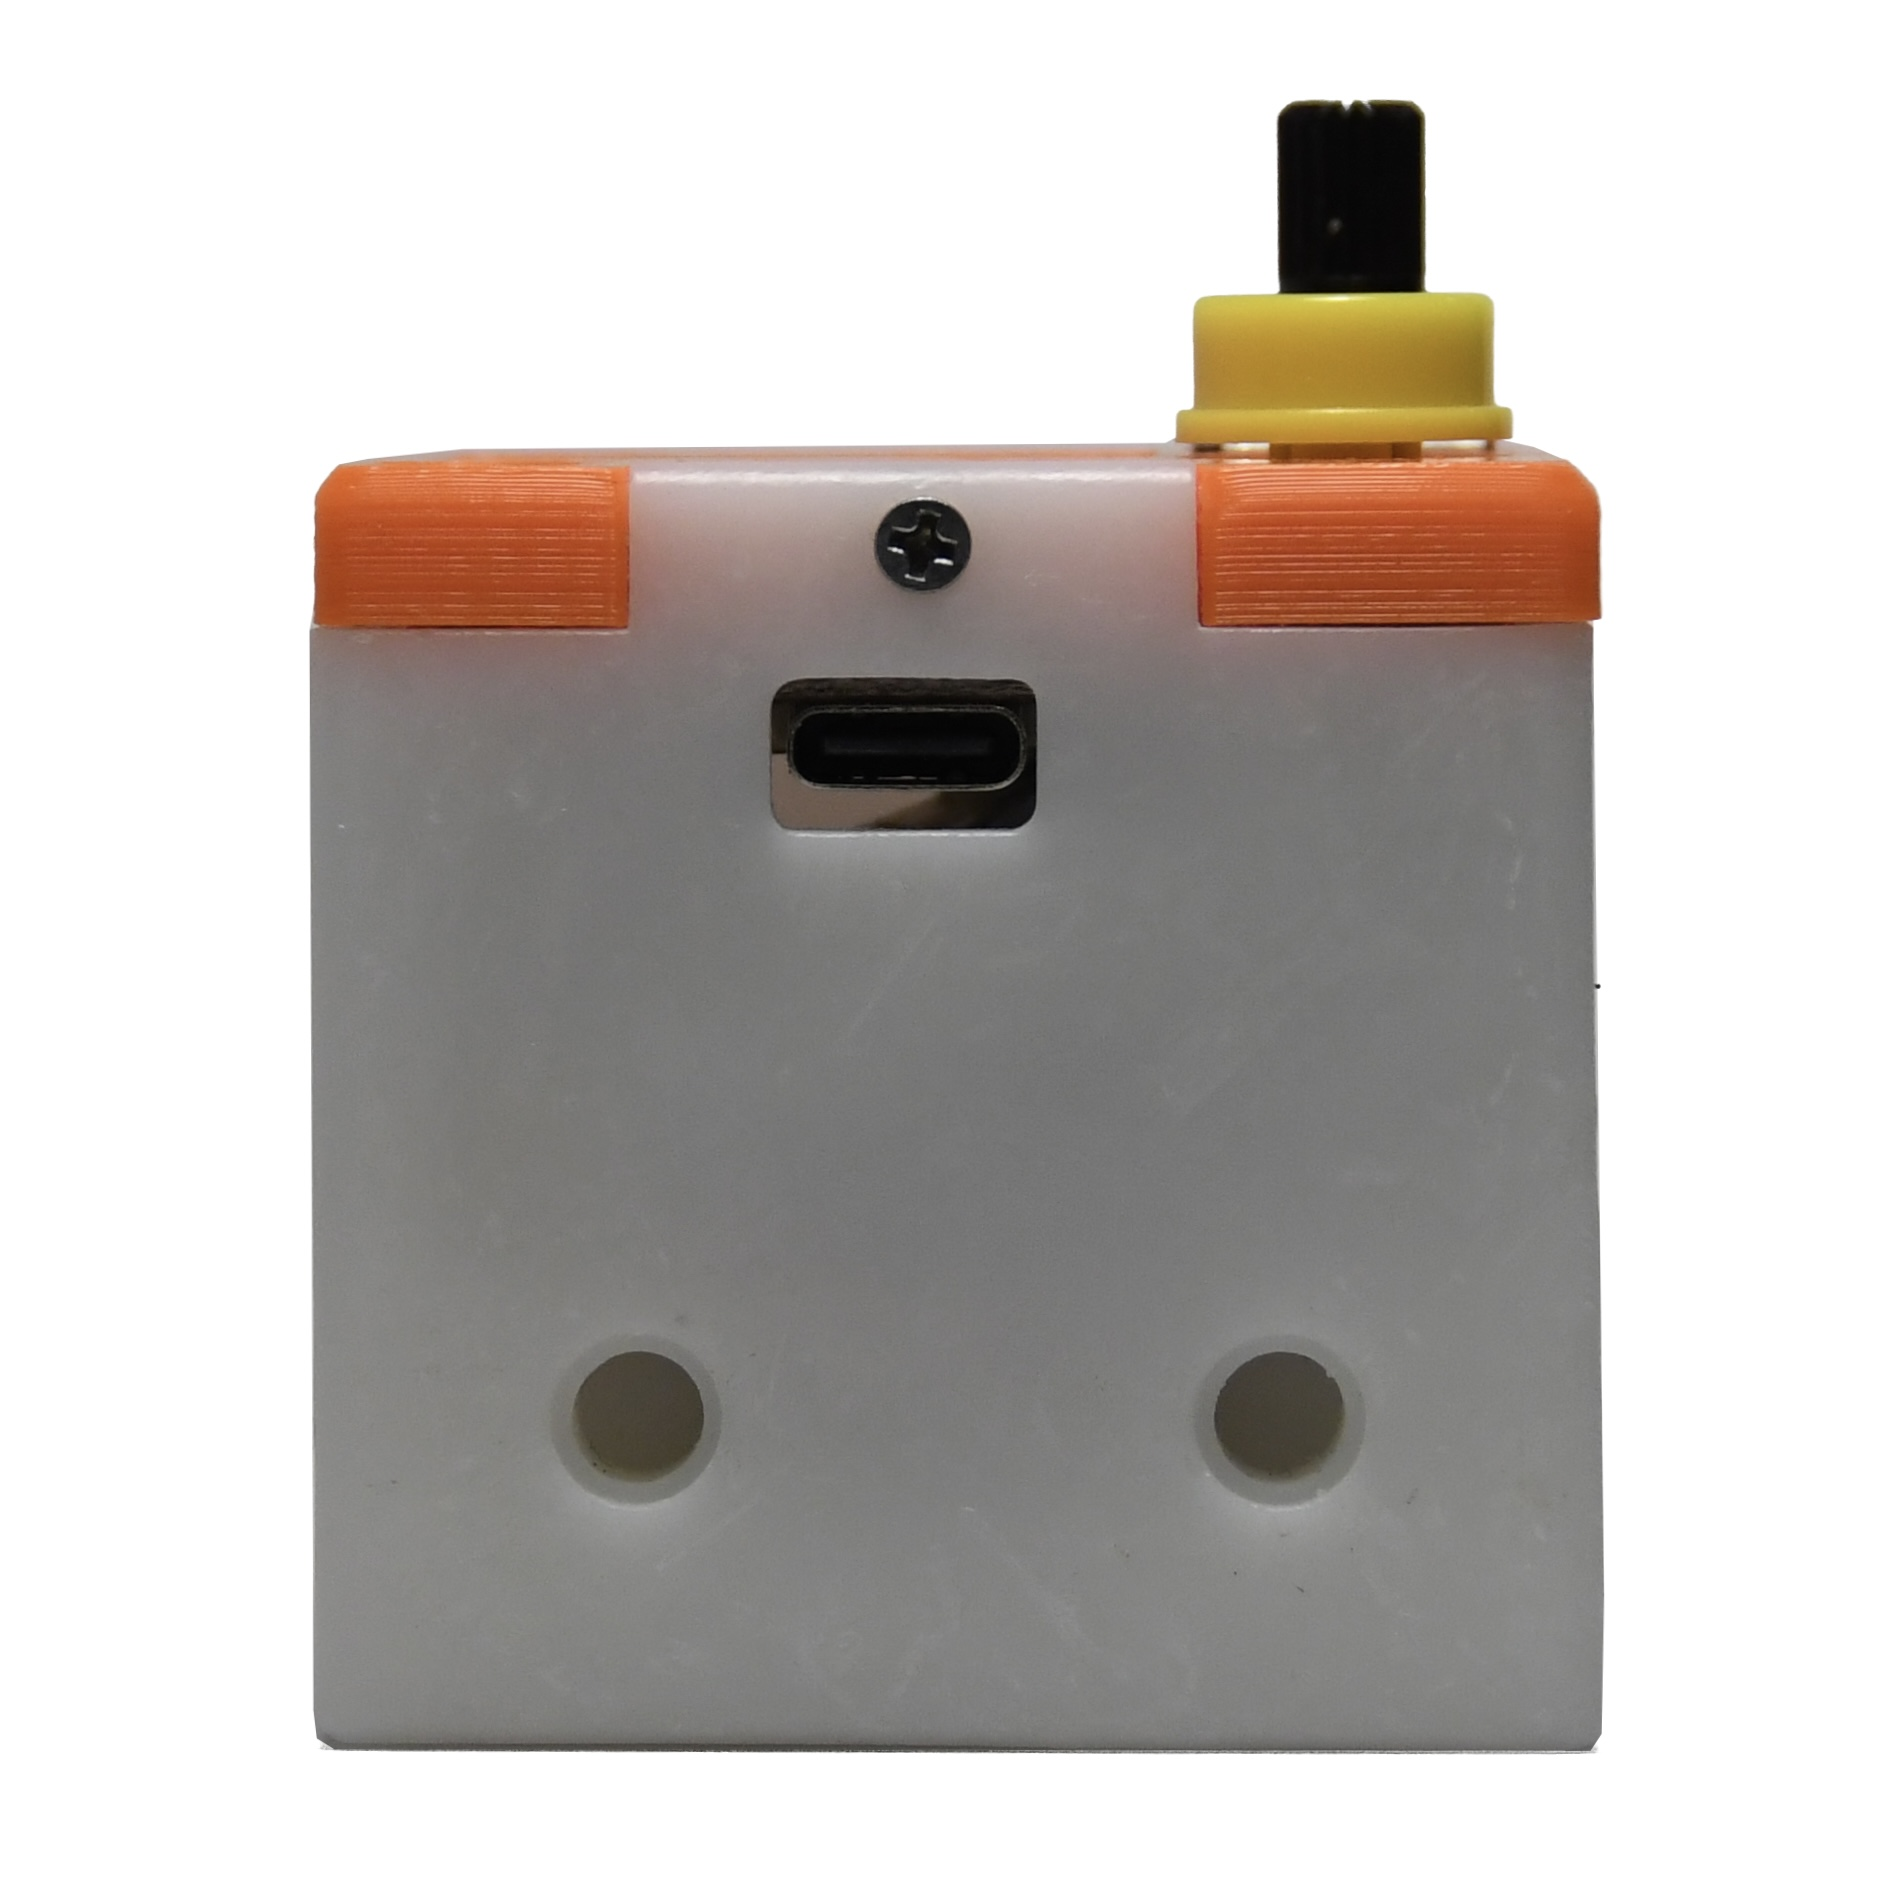
\includegraphics[width=\linewidth]{overleaf/images/sm_bottom.jpg}
    \end{subfigure}
    \\\vspace{\ftspace}
    \caption{Smart Motor v3 displayed from each side. In the first row, from left to right views from the top, front and left are shown, while on the second row, from left to right, views from the right, back and bottom are displayed.}
    \vspace{\ftspace}
    \label{fig:smv3_hardware}
\end{figure}

There are two mechanical interfaces for the Smart Motor v3. One is the motor output, which protrudes from the top of the Smart Motor and is designed to mimic the connection of a LEGO Education motor, allowing LEGO pegs to be connected to the motor output of the Smart Motor. The other is the back of the Smart Motor shell, which is designed to accept LEGO connector pins, allowing components of the LEGO system in play to be attached to the motor or, conversely, the motor to be attached to a LEGO component-based structure. While the system is not directly compatible with LEGO bricks, the dimensions of the shell are approximately the size of a 6x6x5 brick. Specifically, the cube-shaped shell of the Smart Motor v3 is $47\ mm$ x $47\ mm$ x $47\ mm$ (W x B x H), which is the same size as a LEGO brick, making it partially compatible with the LEGO system in terms of pure dimensions. However, in newer iterations, the extrusions added to the side buttons extend beyond this frame, as do the button and potentiometer on the front and the motor on the top of the cube-shaped Smart Motor.

\subsubsection{\label{sec:methods_sm_elec}Electronics Component and Schematics}
The electronical schematics of the Smart Motor v3 closely resembles the general Smart Motor system outlined in Figure \ref{fig:sm_schematic}. The complete electronical system schematics, including all potential components, including wiring, are display in Figure \ref{fig:sm_elec_schematic}.

\begin{figure}[H]
    \centering
    
\includegraphics[width=0.75\linewidth]{overleaf/images/placeholder.png}
    \vspace{\ftspace}
    \caption{Detailed electronic component schematic, including wiring, of the Smart Motor v3 and its custom PCB}
    \label{fig:sm_elec_schematic}
\end{figure}

At the heart of the system is a custom printed circuit board (PCB) called the Dahal Board, which houses a Seeed Studio XIAO ESP32C3 development board, powered by a ESP32C3-series System on Chip (SoC) microcontroller (MC). For simplicity sake, the Seeed Studio XIAO ESP32C3 will be referred to as the microcontroller-board (MCB). The MCB includes a USB-C connector, and the board provides various connection options, such as a Grove-compatible sensor port, two connections for a motor or other analogue outputs, as well as two I2C ports and a battery connection. A variety of components can be connected to the board, although in the case of the Smart Motor, the only fixed connections are to the motor, the screen, which is connected to one of the I2C ports and the battery. The board contains a built-in accelerometer which is used as the default sensor, although it is possible to connect and use other types of sensor to the external sensor port. The board also contains other types of user interface such as an OLED screen, two small buttons, one large button and a potentiometer to allow and enable user interaction directly on the system. A comprehensive list of the Smart Motor v3 components and their price are listed in Table \ref{tab:components}.

\begin{figure}[H]
    \centering
    \begin{subfigure}[b]{0.25\textwidth}
        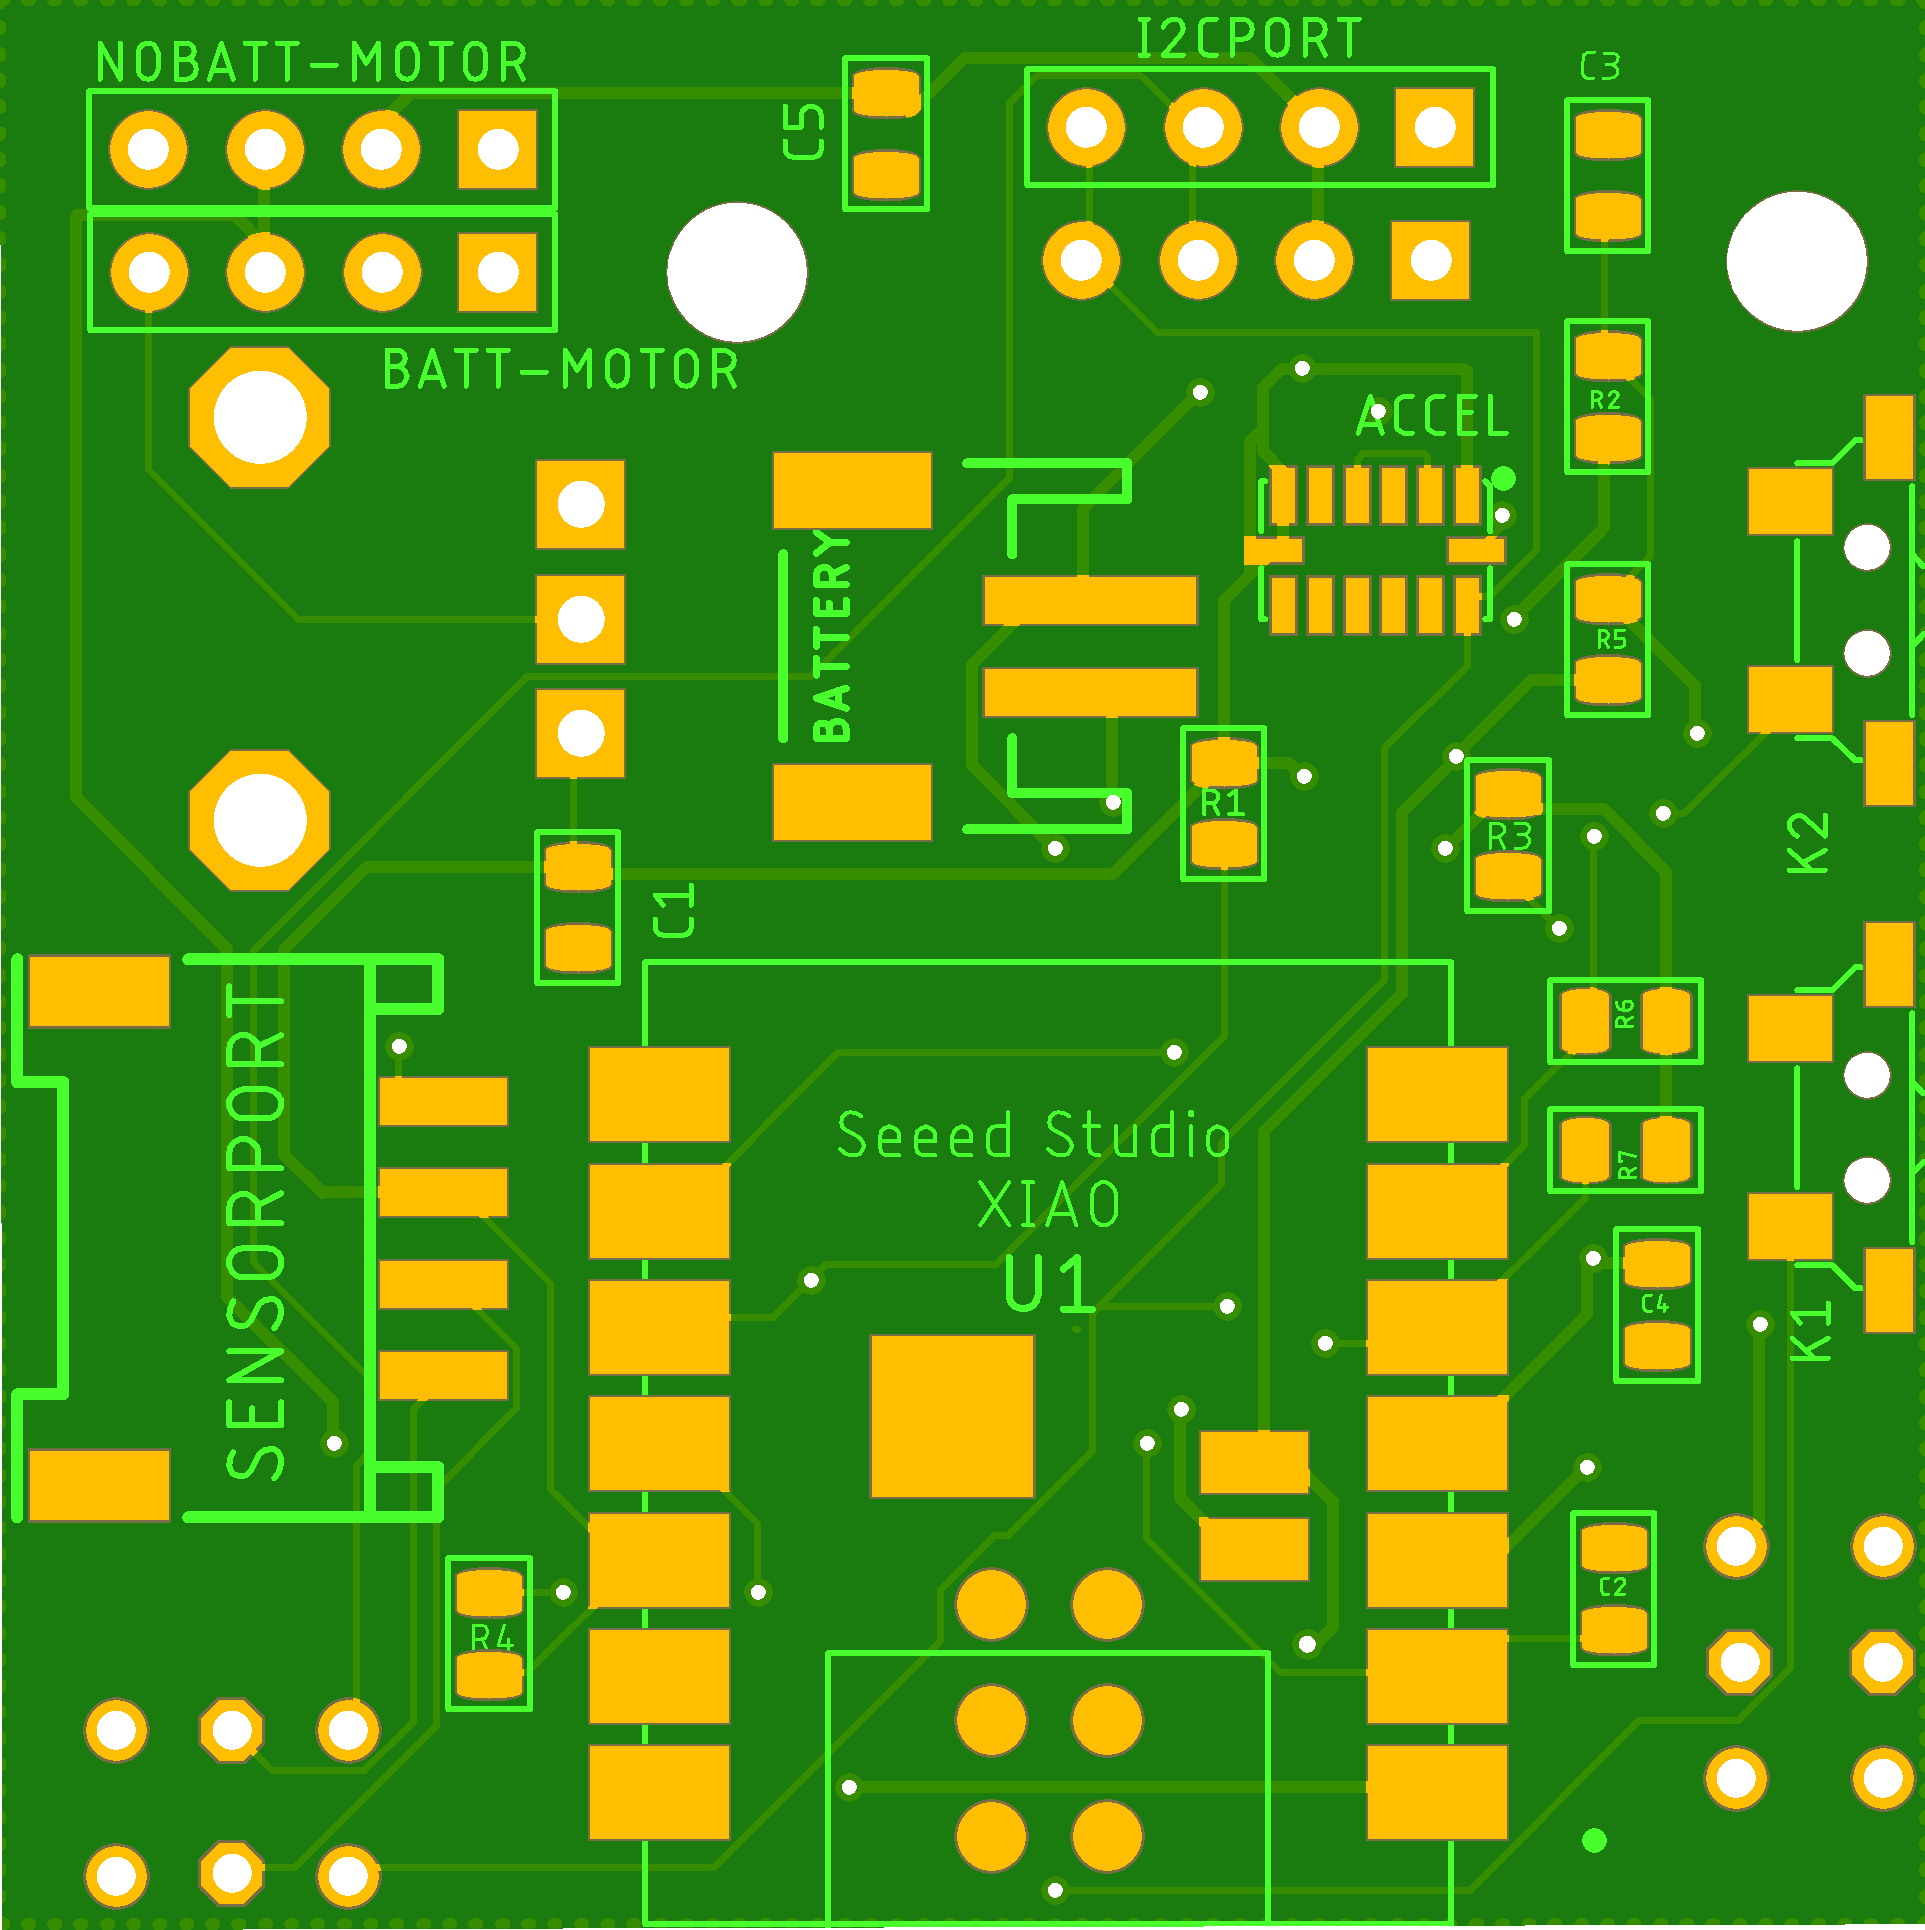
\includegraphics[width=\linewidth]{overleaf/images/pcb_sch.png}
    \end{subfigure}
    \hspace{10pt}
    \begin{subfigure}[b]{0.25\textwidth}
        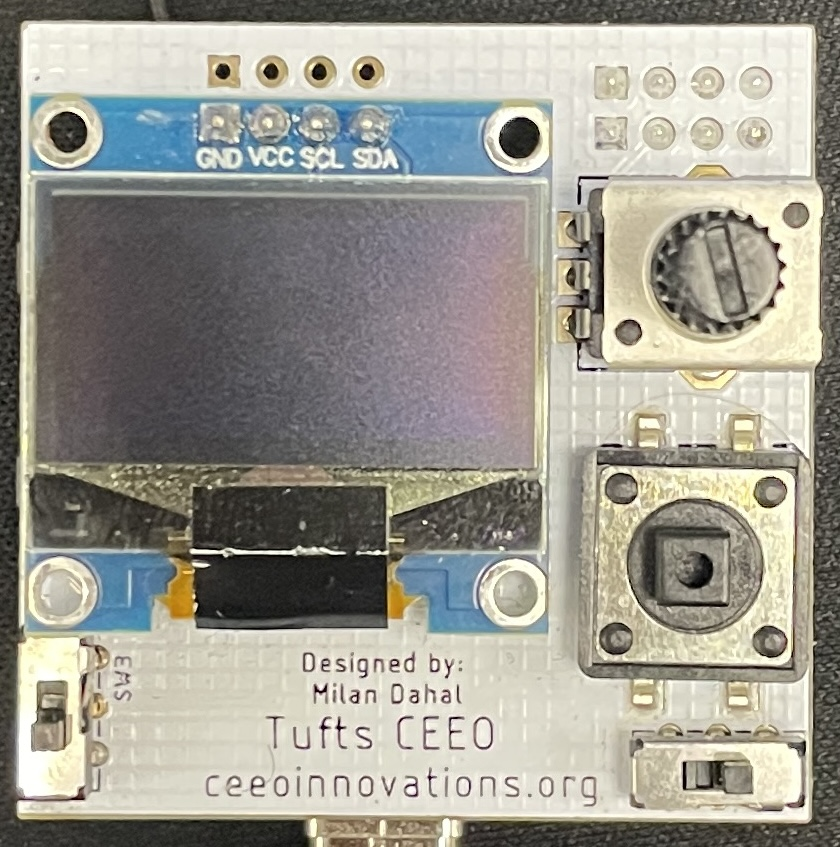
\includegraphics[width=\linewidth]{overleaf/images/front.jpg}
    \end{subfigure}
    \hspace{10pt}
    \begin{subfigure}[b]{0.25\textwidth}
        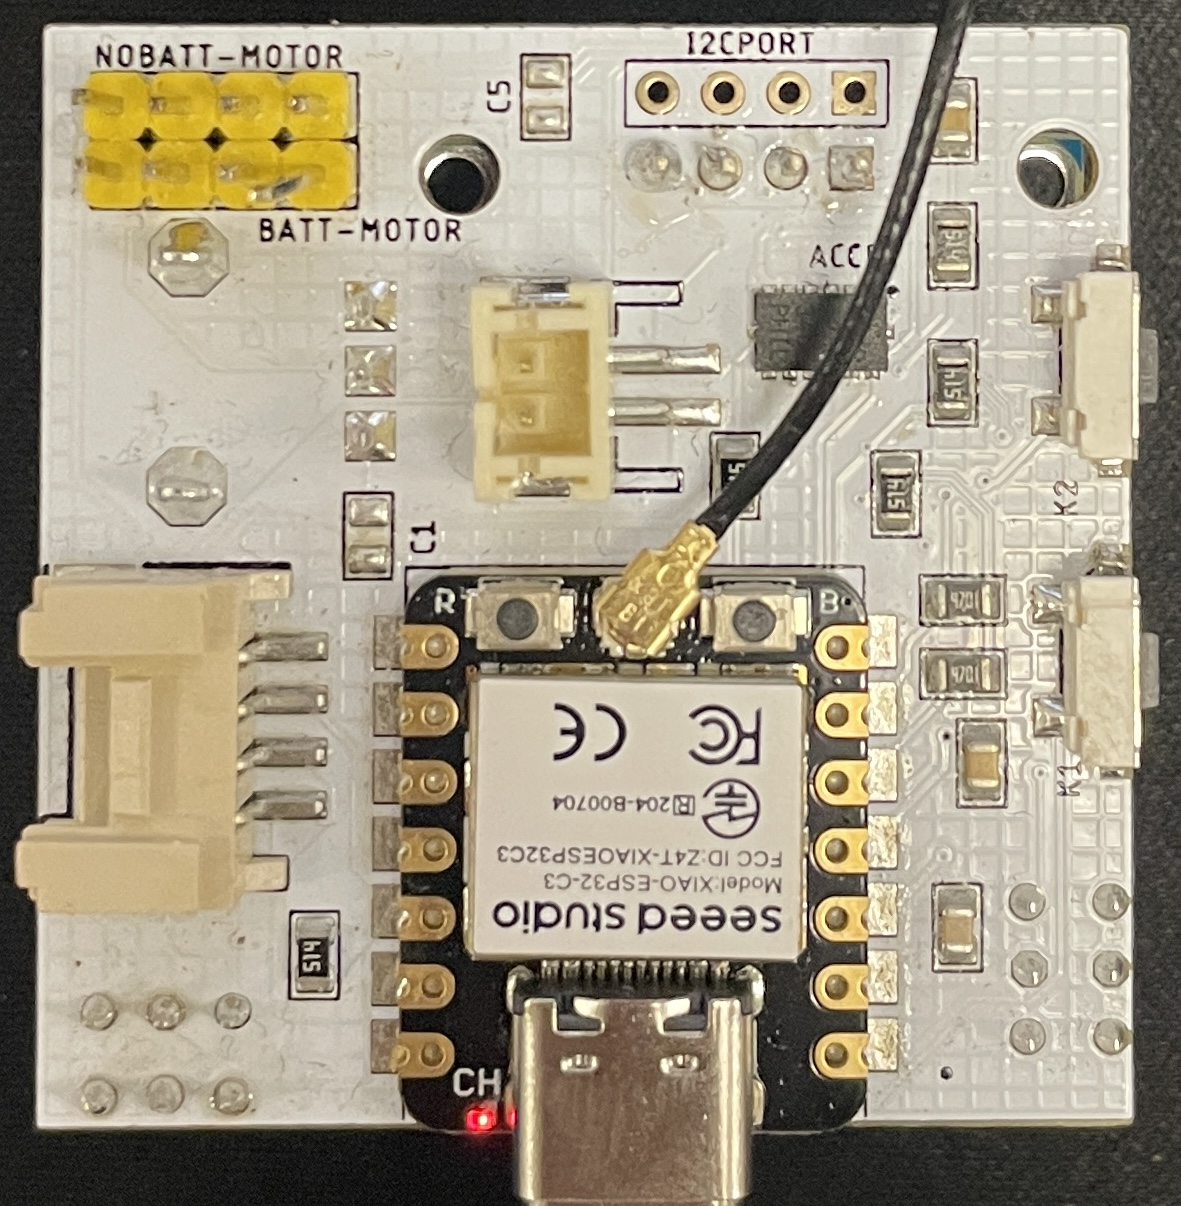
\includegraphics[width=\linewidth]{overleaf/images/back.jpg}
    \end{subfigure}
    \\\vspace{\ftspace}
    \caption{Schematic (left) and image  from top (middle) and bottom (right) of the Smart Motor v3 custom PCB (Dahal Board)}
    \label{fig:sm_dahal_board}
\end{figure}

\begin{table}[H]
    \centering
    \begin{tabular}{|l|p{222pt}|l|}
        \hline
        \textbf{Name} & \textbf{Description} & \textbf{Price (USD)} \\
        \hline
        Dahal Board & Custom PCB, incl. MC, three buttons, a potentiometer, screen, on-board accelerometer and multiple connectors & 16.42 \$\quad\quad \\
        \hline
        \quad Seeed Studio XIAO ESP32C3 & \quad ESP32C3-based MCB (incl. on Dahal Board) & \quad\quad $4.99\ \$$ \\
        \hline
        %\quad ? & \quad Screen (incl. in Dahal Board) & \quad\quad $?\  \$$ \\
        %\hline
        %\quad ? & \quad Button (incl. in Dahal Board) & \quad\quad $?\  \$$ \\
        %\hline
        %\quad ? & \quad Button (incl. in Dahal Board) & \quad\quad $?\  \$$ \\
        %\hline
        %\quad ? & \quad Potentiometer (incl. in Dahal Board) & \quad\quad $?\  \$$ \\
        %\hline
        %\quad ? & \quad Accelerometer (incl. in Dahal Board) & \quad\quad $?\  \$$ \\
        %\hline
        Miuzei MG90S 9G & Servo motor & $2.76\  \$$ \\
        \hline
        Adafruit 4236 & Battery & $6.95\  \$$ \\
        \hline
        % &  &  \\
        %\hline
    \end{tabular}
    \\\vspace{\ftspace}
    \caption{Comprehensive list of all Smart Motor v3 electronic components \citep{dahal_designing_2024}}
    \label{tab:components}
\end{table}

\subsubsection{\label{sec:methods_sm_soft}Software Architecture}
The Smart Motor v3 runs on a slightly adapted version of the MicroPython firmware for ESP32-based MCs, such as the ESP32C3, which allows Python-based code to be run on the chipset. The use of MicroPython brings the advantage of extensive libraries and an active support community, making it easy to use and learn, which in turn makes the system and its code accessible to anyone with basic programming skills and access to a computer and a USB cable.
\\\\
The software that enables the Smart Motor logic to run consists of the main code and libraries to enable and support specific hardware components. All code files and their purpose are listed in Table \ref{tab:smv3_code_list}.

\begin{table}[H]
    \centering
    \begin{tabular}{|l|l|}
        \hline
        \textbf{Name} & \textbf{Purpose} \\
        \hline
        \hline
        boot.py & empty \\
        \hline
        main.py & Main program \\
        \hline
        \hline
        data.py & File with saved data points \\
        \hline
        files.py & Library with logic to read and save to files \\
        \hline
        icons.py & Library with icons for screen \\
        \hline
        log.py & Log output file \\
        \hline
        prefs.py & Preferences file \\
        \hline
        sensors.py & Sensor support library \\
        \hline
        servo & Servo support library \\
        \hline
        ssd1306 & Screen support library \\
        \hline
        version.py & File with version number of all files \\
        \hline
    \end{tabular}
    \vspace{\ftspace}
    \caption{List of all code files contained on the Smart Motor v3 and their purpose.}
    \label{tab:smv3_code_list}
\end{table}

The main program contains all the logic necessary for the Smart Motor to function as intended. It sets up and configures all the pins of the ESP32C3 chipset and initialises all the connected components, including the sensors, the motor and the user interface, which includes the screen, the main and two side buttons and the potentiometer. In the case of sensors, it detects whether an external sensor is present and, if not, defaults to using the on-board accelerometer. It also defines the different modes required, training and playing, and sets up the UI logic. It further sets up the button-press handlers and their logic and links the potentiometer to the motor output in the case of training mode. It also defines the ML principle and hosts the nearest neighbour algorithm that determines the motor output based on the current sensor input and training data for the game mode.
The further code files host various libraries and supporting code for the different components.

\subsubsection{\label{sec:methods_sm_ui}User Interface and Interaction Design}

One of the key design features of the Smart Motor concept is for the Smart Motor to used as a stand-alone unit, hence be trainable directly on the device, without the need of any supporting materiel. To this extent \citet[]{dahal_designing_2024} has come up with an interaction design and UI, enabling interaction of a user with the Smart Motor system. In the case of the Smart Motor v3, the UI includes a screen to display information in a graphic way, the two side buttons, used for navigation, the main button, used as a select button and a potentiometer, which in the training mode is linked to the motor, and used to set the motor position or speed.

\begin{figure}[H]
    \centering
    \begin{subfigure}[b]{0.19\textwidth}
        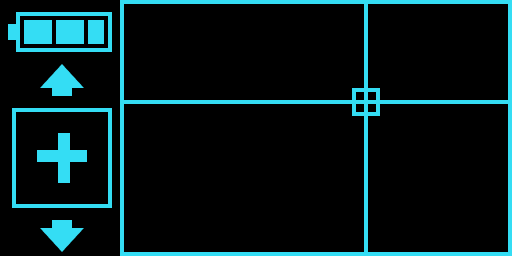
\includegraphics[width=\linewidth]{overleaf/images/train.png}
        \caption{Training screen:\\Add data-point\\\quad}
    \end{subfigure}
    \begin{subfigure}[b]{0.19\textwidth}
        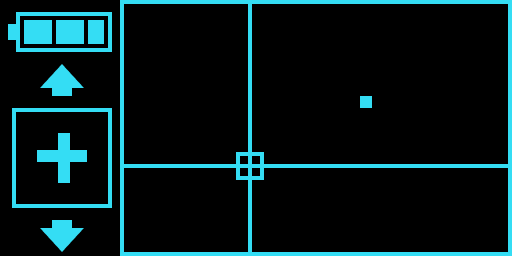
\includegraphics[width=\linewidth]{overleaf/images/add.png}
        \caption{Training screen:\\Add data-point,\\One added point}
    \end{subfigure}
    \begin{subfigure}[b]{0.19\textwidth}
        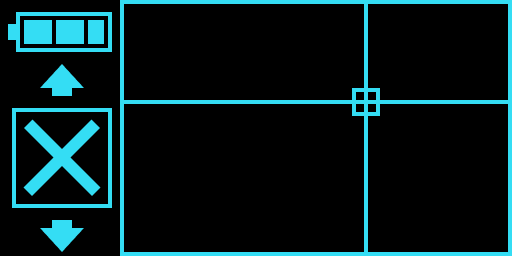
\includegraphics[width=\linewidth]{overleaf/images/remove.png}
        \caption{Training screen:\\Remove data-point\\\quad}
    \end{subfigure}
    \begin{subfigure}[b]{0.19\textwidth}
        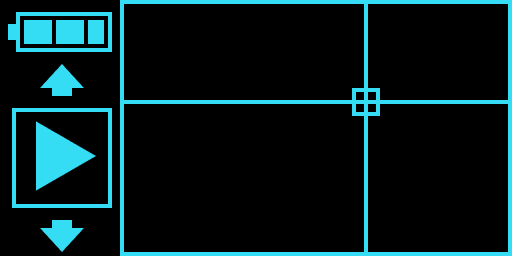
\includegraphics[width=\linewidth]{overleaf/images/trainplay.png}
        \caption{Training screen:\\Start playing mode\\\quad}
    \end{subfigure}
    \begin{subfigure}[b]{0.19\textwidth}
        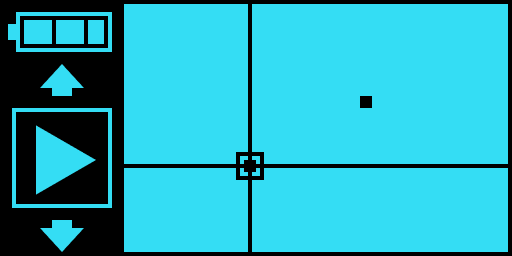
\includegraphics[width=\linewidth]{overleaf/images/play.png}
        \caption{Playing screen:\\Two data-points\\\quad}
    \end{subfigure}
    \vspace{\ftspace}
    \caption{Screen UI for training- (a-d) and playing-mode (e) \citep[from][p. 40-41]{dahal_designing_2024}}
    \label{fig:screen}
\end{figure}

The design of the visual information on the screen, as shown in Figure \ref{fig:screen}, includes a battery indicator in the top left, an action indicator in the middle to bottom left, and spanning the rest of the screen is a two-dimensional plot showing the current motor position on the X-axis and the current sensor reading on the Y-axis in the form of lines. There is a small crosshair where these two lines meet. In training mode, which the SM v3 enters per default when starting up, there are three possible actions, with the current action being displayed by the action indicator. Switching between the actions is possible using the side button, while confirming the action can be done using the select button. 
\begin{enumerate}
    \item Adding Data-point:\\
    Training data, in the form of data points (linking a particular sensor reading to a particular motor position) can be added using the Select button, which adds a point at the location of the crosshairs using the current value of the motor and sensor, as shown in Figure \ref{fig:screen} (a). An added data point is displayed as a point on the graph at the position where the motor position value on the X-axis meets the sensor value on the Y-axis, as seen in Figure \ref{fig:screen} (b). These points represent the training data for the Smart Motor, which is used in its play mode to determine the motor output based on a sensor input using the nearest neighbour algorithm.
    \item Removing Data-point:\\
    Added data points can be removed using the remove action, shown in Figure \ref{fig:screen} (c), with data-points being removed in the reverse order of them being added.
    \item Enter Playing Mode:\\
    With the third action playing mode can be entered, as displayed in Figure \ref{fig:screen} (d). The playing mode is displayed as shown in Figure \ref{fig:screen} e. To exit the playing mode, the select button can be used to return to the screen in Figure \ref{fig:screen} (d) or one can directly use the side buttons to select a different action, which exits the playing mode in favour of training mode.
\end{enumerate}

\subsection{\label{sec:methods_tech_review}Technology and Literature Review}

 Most of the hardware, with the exception of the PCB and the Smart Motor v3 shell, are off-the-shelf components. As such, they inherently have more capability and application potential due to their general purpose design, which is particularly true for the ESP32C3-based MCB, which is examined in detail. ESP32C3 SoC-enabled networking options are also explored, such as Bluetooth and Wi-Fi, including previous work and solutions developed in this field, and finally the Seeed Studio Grove sensors are given brief consideration.

\subsubsection{\label{sec:rev_esp}ESP32 System-on-Chip Family}

ESP32 refers to a family of SoCs designed and developed by Espressif Systems, starting with the ESP32 series of SoCs, originally manufactured by Taiwan Semiconductor Manufacturing Company Limited (TSMC) using their $40\ nm$ process \citep{espressif_systems_esp32_2025}.
Further series have been developed and released over time, including the ESP32C3 and ESP32C6 series, which Seeed Studio has used to develop the corresponding XIAO development boards. The first of these, the ESP32C3-based MCB, is of particular interest due to its use in the SM v3, though consideration will also be given to the newer ESP32C6-based MCB. Although even newer series of the SoC, such as the ESP32C5 and ESP32C61, have been announced \citep{espressif_systems_esp_nodate}, their respective datasheets have not yet been released, nor is there any indication of development of the respective development boards by Seeed Studio at the time of writing.\\

% \begin{figure}[H]
%     \centering
%     \begin{subfigure}{0.15\textwidth}
%         
\includegraphics[width=\linewidth]{overleaf/images/placeholder.png}
%     \end{subfigure}
%     \hspace{10pt}
%     \begin{subfigure}{0.15\textwidth}
%         
\includegraphics[width=\linewidth]{overleaf/images/placeholder.png}
%     \end{subfigure}
%     \\\vspace{\ftspace}
%     \caption{ESP32C3 SoC (left) and ESP32C6 SoC (right)}
%     \label{fig:ESP32soc}
% \end{figure}

\textbf{Seeed Studio XIAO ESP32C3}\\\\
The Seeed Studio XIAO ESP32C3 is a compact development board based on the ESP32C3 SoC. This MCB is designed to leverage the key features of the ESP32C3, in particular its wireless connectivity capabilities. At its core, the board uses a 32-bit RISC-V CPU and supports both IEEE Standard 802.11b, -g and -n (Wi-Fi 4) and Bluetooth Low Energy (BLE) of the Bluetooth 5.0 standard. 
In terms of interfaces, the chip provides four serial interfaces, including two UART, one I2C and one SPI, as well as eleven GPIO pins (which can be used for PWM), four ADC pins and one JTAG bonding pad interface. 
The board's design incorporates a small form factor with a single-sided surface mount layout, which is how it is mounted on the Dahal board. The board also includes a Hirose U.FL antenna interface for its wireless functionality. For user interaction, the MCB includes a small reset button and a bootloader mode button, as well as an LED indicator for the USB-C interface. The MCB's layout, pin-out and images are shown in Figure \ref{fig:esp32c3}, while a summary of the MCB's and MC's specifications can be found in Table \ref{tab:esp_comparison}. \citep{espressif_systems_esp32-c3_2024, seeed_studio_seeed_2024-2}

\begin{figure}[H]
    \centering
    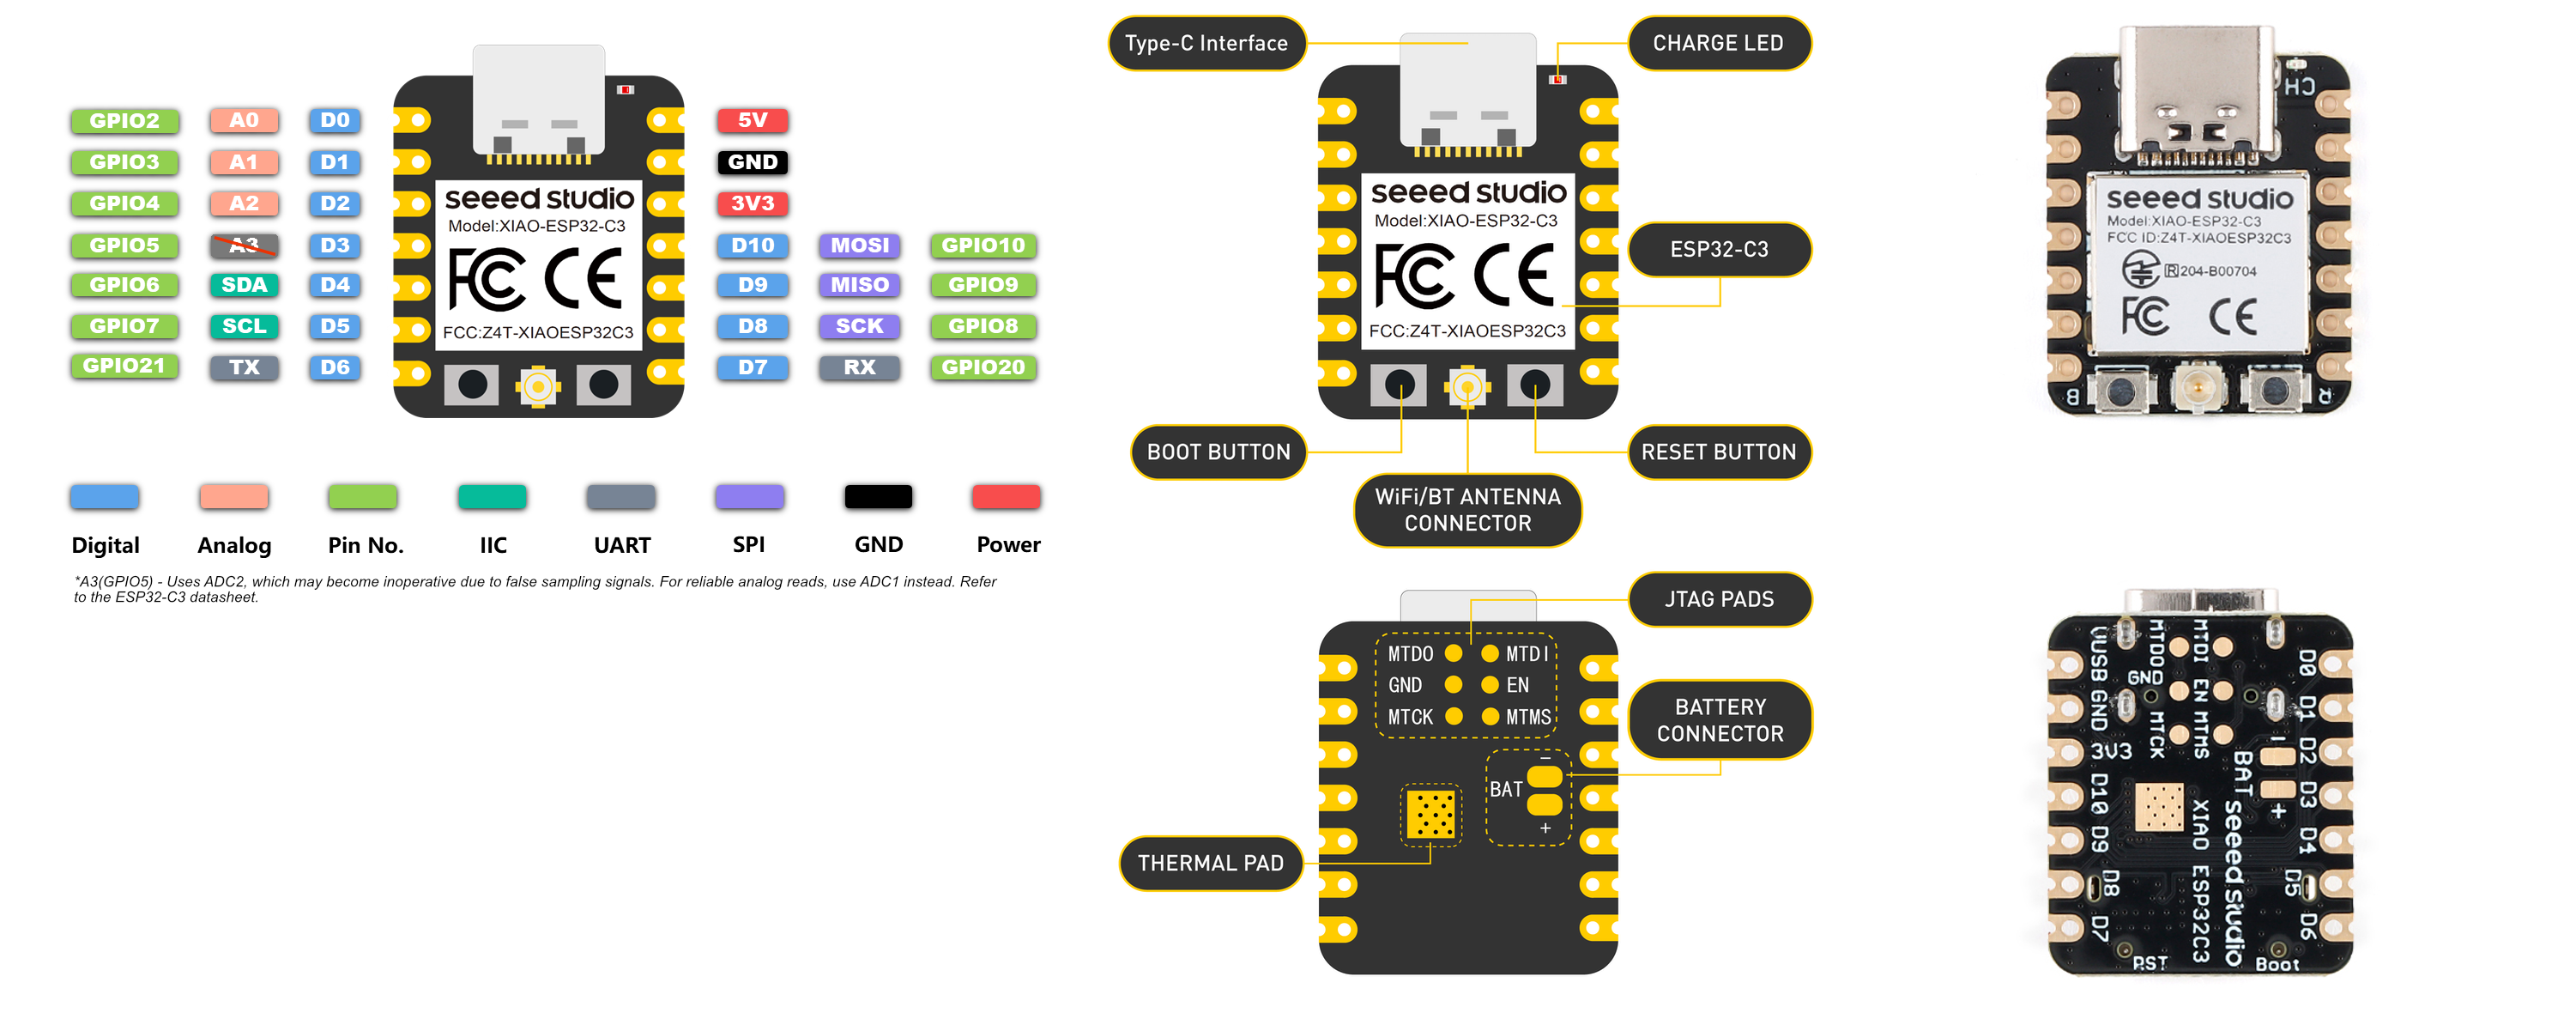
\includegraphics[width=0.75\textwidth]{overleaf/images/xiaoesp32c3.png}
    \\\vspace{\ftspace}
    \caption{Seeed Studio XIAO ESP32C3 pin-out schematic (left), layout (middle) and image(right) \citep[adapted from][]{seeed_studio_seeed_2024-2}}
    \label{fig:esp32c3}
\end{figure}

\textbf{Seeed Studio XIAO ESP32C6}\\\\
The Seeed Studio XIAO ESP32C6 is a compact development board based on the ESP32C6 SoC. This MCB is designed to leverage the key features of the ESP32C6, in particular its wireless connectivity capabilities. At its core, the board uses two 32-bit RISC-V CPUs and supports the IEEE Standard 802.11ax (Wi-Fi 6), BLE of the Bluetooth 5.3 standard and IEEE Standard 802.15.4 (Zigbee and Thread).
In terms of interfaces, the chip provides four serial interfaces, including one UART, one I2C, one LP\_I2C and one SPI, as well as eleven GPIO pins (which can be used for PWM), seven ADC pins, one SDIO interface. The board's design incorporates a small form factor. 
The board also includes an on-board antenna, as well as a Hirose U.FL antenna interface for its wireless functionality. For user interaction, the MCB includes a small reset button and a bootloader mode button, as well as an LED indicator for the USB-C interface. The MCB's layout, pin-out and images are shown in Figure \ref{fig:esp32c6}, while a summary of the MCB's and MC's specifications can be found in Table \ref{tab:esp_comparison}.  \citep{espressif_systems_esp32-c6_2024, seeed_studio_seeed_2024-1}
\begin{figure}[H]
    \centering
    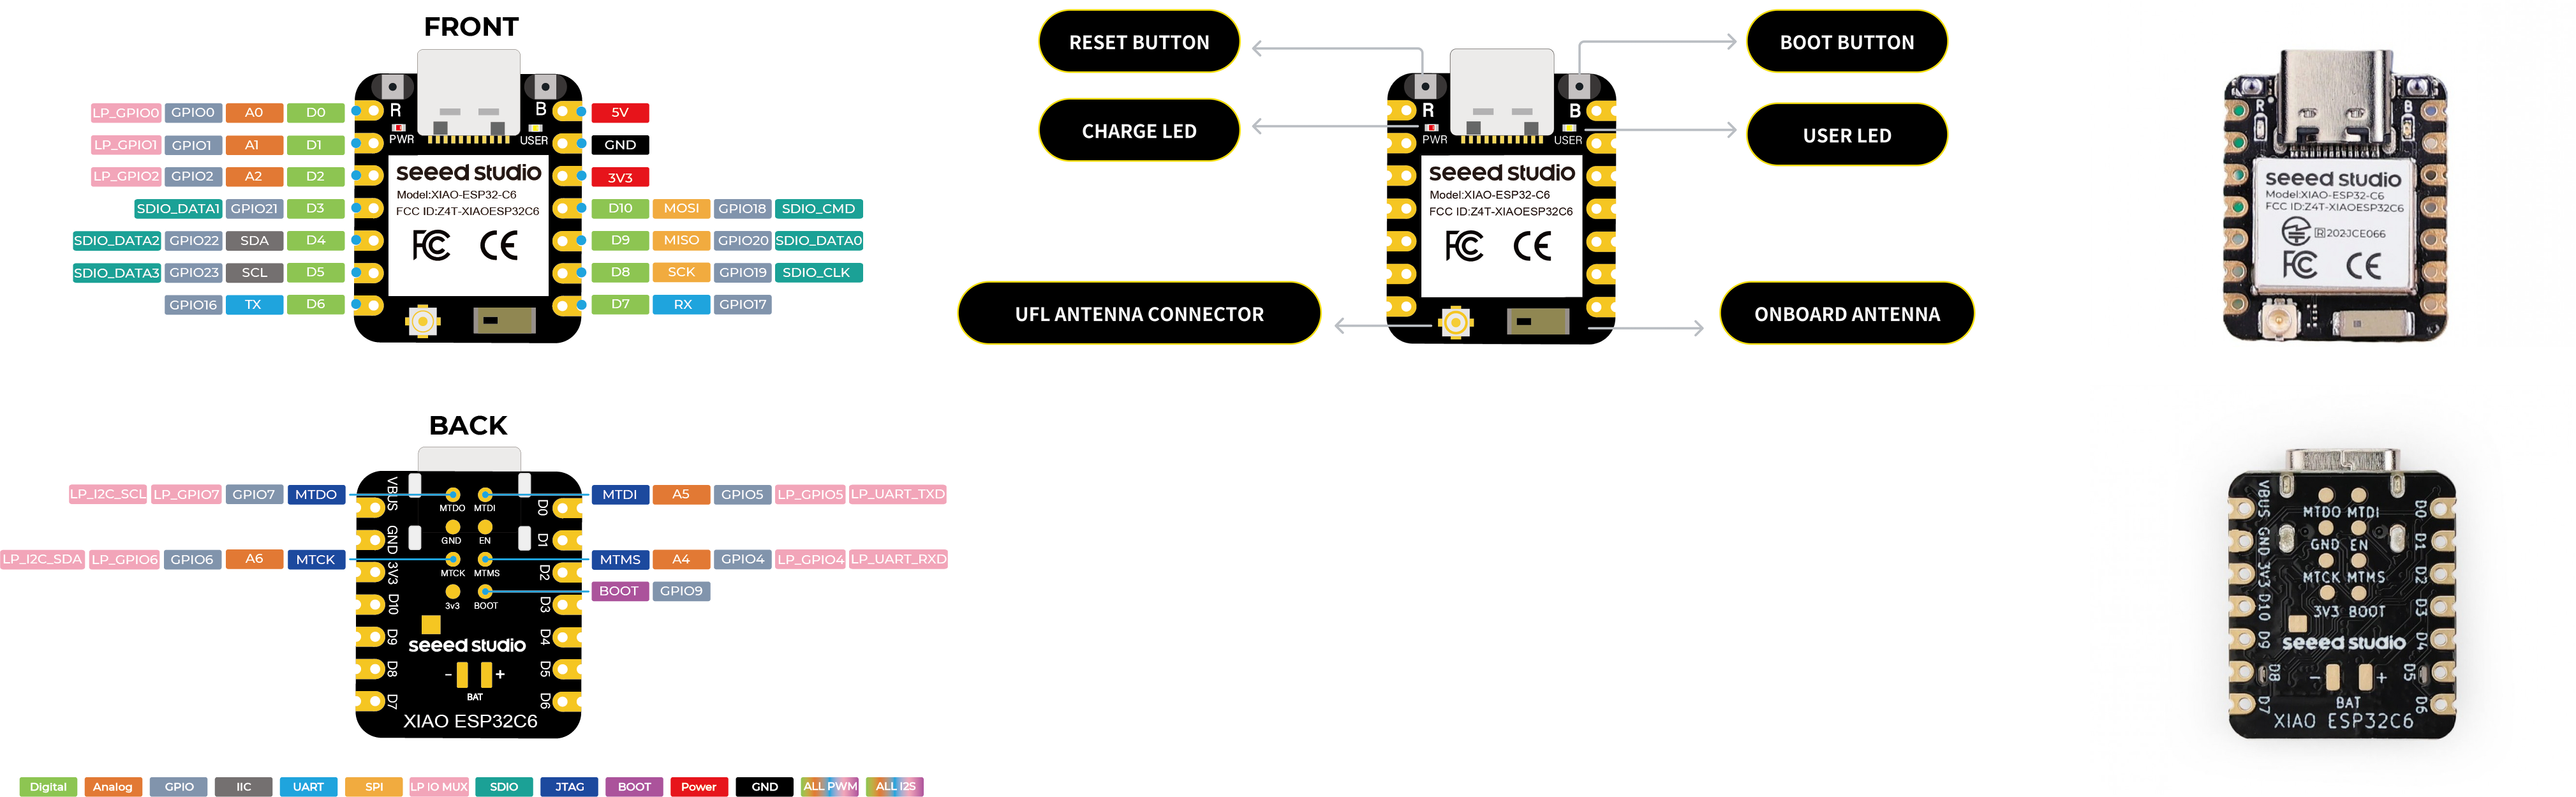
\includegraphics[width=\textwidth]{overleaf/images/xiaoesp32c6.png}
    \\\vspace{\ftspace}
    \caption{Seeed Studio XIAO ESP32C6 pin-out schematic (left), layout (middle) and image (right) \citep[adapted from][]{seeed_studio_seeed_2024-1}}
    \label{fig:esp32c6}
\end{figure}

\begin{table}[H]
\begin{tabular}{|m{35pt}|m{55pt}|p{160pt}|p{175pt}|}
\hline
\multicolumn{2}{|c|}{\textbf{Products}} & \textbf{XIAO ESP32C6} & \textbf{XIAO ESP32C3} \\\hline
\multicolumn{2}{|c|}{\multirow{2}{*}{\textbf{Processor}}} & Espressif ESP32-C6 SoC & Espressif ESP32-C3 SoC \\\cline{3-4}
\multicolumn{2}{|c|}{} & Two 32-bit RISC-V processors, with the high-performance one running up to 160 MHz, and the low-power one clocking up to 20 MHz & RISC-V single-core 32-bit chip processor with a four-stage pipeline that operates at up to 160 MHz \\\hline
\multirow{4}{*}{\rotatebox{90}{\textbf{Wireless}}} & \textbf{Wi-Fi} & 2.4GHz Wi-Fi 6 subsystem & 2.4GHz Wi-Fi 4 subsystem \\\cline{2-4}
& \textbf{BLE} & Bluetooth 5.3, Bluetooth Mesh & Bluetooth 5.0, Bluetooth Mesh \\\cline{2-4}
& \textbf{Other} & Zigbee, Thread, IEEE 802.15.4 & / \\\cline{2-4}
& \textbf{Antenna} & U.FL interface with ext. antenna & On-board antenna + U.FL interface \\\hline
\multicolumn{2}{|c|}{\textbf{On-chip Memory}} & 512kB SRAM \& 4MB Flash & 400kB SRAM \& 4MB Flash \\\hline
\multicolumn{2}{|c|}{\multirow{2}{*}{\textbf{Interface}}} & 1x UART, 1x LP\_UART, 1x I2C, 1x LP\_IIC, 1x SPI, 11x GPIO(PWM),   7x ADC, 1x SDIO & 2x UART, 1x I2C, 1x SPI, 11x GPIO(PWM), 4x ADC \\\cline{3-4}
\multicolumn{2}{|c|}{} & \multicolumn{2}{c|}{1x Reset button, 1x Boot button} \\\hline
\multicolumn{2}{|c|}{\textbf{Dimensions}} & \multicolumn{2}{c|}{21 x 17.8 mm} \\\hline
\multirow{3}{*}{\rotatebox{90}{\textbf{Power}}} & \textbf{Input voltage} & \multicolumn{2}{l|}{\makecell{Type-C: 5V \\ BAT: 4.2V}} \\\cline{2-4}
 & \textbf{Circuit operating Voltage} & \multicolumn{2}{l|}{\makecell{USB:5V@9mA \\ BAT:3.8V@9mA}} \\\cline{2-4}
 & \textbf{Charging battery current} & 100mA & 350mA \\\hline
\multirow{3}{*}{\rotatebox{90}{\makecell{\quad\textbf{Power Consumption Model} \\ \quad\textbf{(Supply Power: 3.8V)}}}} & \textbf{Modem-sleep Model} & $\sim$30 mA & $\sim$24 mA \\\cline{2-4}
 & \textbf{Light-sleep Model} & $\sim$2.5 mA & $\sim$3 mA \\\cline{2-4}
 & \textbf{Deep Sleep Model} & $\sim$15 \micro A & $\sim$44 \micro A \\\hline
\multicolumn{2}{|c|}{\textbf{Working Temperature}} & \multicolumn{2}{c|}{-40°C $\sim$85°C} \\\hline
\end{tabular}
\vspace{\ftspace}
    \caption{Specification comparison of the ESP32C3 SoC- and ESP32C6 SoC-based MCB \citep[adapted from][]{seeed_studio_seeed_2024-2,seeed_studio_seeed_2024-1}}
    \label{tab:esp_comparison}
\end{table}

\subsubsection{\label{sec:rev_net}Networking}

Both the ESP32C3 SoC- and ESP32C6 SoC-based MCBs come with built in Bluetooth and Wi-Fi wireless networking capabilities, the latter of the two MBCs even includes additional hardware and support for the IEEE Standard 802.15.4 \citep{noauthor_ieee_2024} for low‐rate wireless networks. Both MCBs come with an antenna connector, with the latter even including a small on-board antenna.\\

\textbf{Bluetooth and Bluetooth Low Energy}\\\\
Bluetooth is a short-range wireless transmission technology standard, operating in the $2.4-2.485\ GHz$ industrial, scientific, and medical (ISM) radio band, with a radio class-dependant range of approximately 1 meter, 10 meters and 100 meters for Class 1, Class 2 and Class 3 respectively \citep[see][]{noauthor_basics_2012}. The standard was developed and is maintained by the Bluetooth Special Interest Group, which includes various companies as members. While initial specifications of Bluetooth were adopted by the Institute of Electrical and Electronics Engineers (IEEE) as part of the IEEE Standard 802.15 in 2002 \citep[Bluetooth 1.1,][]{noauthor_ieee_2002} and 2005 \citep[Bluetooth 1.2,][]{noauthor_ieee_2005}, these standards have since been withdrawn, with them instead maintained and released directly by the Bluetooth Special Interest Group. 
In addition to the classic Bluetooth protocol, with the release of the Bluetooth 4.0 standards, Bluetooth Low Energy (BLE) was introduced as a separate entity. As the name suggests, BLE is intended as a low-energy version of the classic Bluetooth for internet of things (IoT) applications \citep{noauthor_bluetooth_2017}.
While both classic Bluetooth and BLE maintain full backwards compatibility with earlier versions, the two protocols are not compatible with each other, though they can co-exist on the same device. \citep{noauthor_bluetooth_nodate}

\begin{table}[H]
    \centering
    \begin{tabular}{|l|l|l|}
        \hline
        \textbf{Feature} & \textbf{ESP32C3} & \textbf{ESP32C6} \\\hline
        Bluetooth version & Bluetooth 5.0 Low Energy & Bluetooth 5.3 Low Energy \\\hline
        Maximum data rate & 2 Mbps & 2 Mbps \\\hline
        Frequency band & 2.4 GHz & 2.4 GHz \\\hline
        Frequency range & 2402 MHz & 2480 MHz \\\hline
        %Channel width &  &  \\\hline
        Range & Up to 4x of Bluetooth 4.2 & Up to 4x of Bluetooth 4.2 \\\hline
        Advertising channels & 3 & 3 \\\hline
    \end{tabular}
    \vspace{\ftspace}
    \caption{Specifications of Bluetooth standards found on the ESP32C3 and ESP32C6 SoCs \citep{noauthor_bluetooth_2024-1, noauthor_bluetooth_2024-2}}
    \label{tab:esp_bluetooth}
\end{table}
%\textbf{BLE on the ESP32C3 and ESP32C6}\\\\
The ESP32C3 supports BLE standards up to version Bluetooth 5.0 \citep{espressif_systems_esp32-c3_2024, seeed_studio_seeed_2024-2, noauthor_bluetooth_2024-2}, while the ESP32C6 supports BLE standards up to version Bluetooth 5.3 \citep{espressif_systems_esp32-c6_2024, seeed_studio_seeed_2024-1, noauthor_bluetooth_2024-1}. An overview of the two technologies is listed in Table \ref{tab:esp_bluetooth}.\\

\textbf{ESP-BLE-MESH}\\\\
The ESP32C3 and ESP32C6 SoCs' support for BLE adds support for Bluetooth Mesh. Bluetooth Mesh is a device mesh networking protocol based on BLE \citep{noauthor_bluetooth_2023, noauthor_bluetooth_2023-1}. Building on Bluetooth Mesh, Espressif Systems has developed ESP-BLE-MESH, a Bluetooth Mesh implementation specifically for ESP32 based devices.
Once formed, the ESP-BLE-MESH can become a large scale (1000+) interconnected peer-to-peer mesh. Nodes are connected to all other nodes within their range, with the topology of the network determined by heartbeat messages sent by nodes and received by other nodes in their vicinity. A mesh does not form automatically, but requires provisioning: to add nodes to the mesh, they must be provided with the necessary information and cryptographic key via a provisioning device, such as a smartphone.  
In terms of message transmission, ESP-BLE-MESH uses a controlled flooding approach, which means that a node sends a message to all other nodes to which it is connected. Specially designated gateway nodes forward the message to all their connected nodes, and so on. As the ESP-BLE-MESH is a fully interconnected mesh, there are many overlapping connections and routing possibilities, so in a controlled flooding approach a message is received by sheer brute force, with the possibility of nodes receiving the same message more than once, creating redundancy at the cost of inefficient routing and high network load. The ESP-BLE-MESH implementation is available for use with ESP32-based devices using the Espressif IoT Development Framework (ESP IDF) and standard ESP AT firmware, but there is currently no library implementation for ESP32 devices using MicroPython firmware. \citep{espressif_systems_esp-ble-mesh_nodate, noauthor_bluetooth_2023, noauthor_bluetooth_2023-1}\\

\textbf{Wi-Fi}\\\\
Wi-Fi is a family of wireless transmission technologies that enable wireless local area networks (WLANs), based on the original IEEE Standard 802.11 and its amendments \citep[][]{noauthor_ieee_2024}, and certified for interoperability by the Wi-Fi Alliance \citep{noauthor_certification_2020}. The Wi-Fi Alliance, like the Bluetooth Special Interest Group, is a membership-based group of companies that includes most of the manufacturers of IEEE Standard 802.11-based technology. \citep{noauthor_wi-fi_nodate} Wi-Fi operates in the $2.4\ GHz$ ISM band, the same band used by Bluetooth, although newer versions also use the 5 GHz and 6 GHz frequency bands. Range and transmission bandwidth are highly dependent on the specific IEEE standard used, which usually corresponds to the Wi-Fi generation. Wi-Fi generations are mostly backwards compatible with earlier generations and standards.

\begin{table}[H]
    \centering
    \begin{tabular}{|l|l|l|}
        \hline
        & \textbf{ESP32C3} & \textbf{ESP32C6} \\\hline
        Wi-Fi Generation & Wi-Fi 4 & Wi-Fi 6 \\\hline
        IEEE Standard & 802.11n & 802.11ax \\\hline
        Maximum data rate & 600 Mbps & 9.6 Gbps \\\hline
        Frequency band & 2.4 GHz & 2.4 GHz \\\hline
        Frequency range & 2402-2482 MHz & 2402-2482 MHz \\\hline
        Channels & 13, 11 & 13, 11 \\\hline
        Channel width & 20, 40 MHz & 20, 40 MHz \\\hline
        MIMO streams & Up to 4 & Up to 8 \\\hline
        Modulation & Up to 64-QAM & Up to 1024-QAM \\\hline
        %OFDMA & No & Yes \\\hline
        %Target Wake Time & No & Yes \\\hline
        %MU-MIMO & No & Yes (Uplink and Downlink) \\\hline
    \end{tabular}
    \vspace{\ftspace}
    \caption{Specifications of Wi-Fi standards as implemented on the ESP32C3 and ESP32C6 SoCs \citep{noauthor_ieee_2009, noauthor_ieee_2021}}
    \label{tab:esp_wifi}
\end{table}

%\textbf{Wi-Fi on the ESP32C3 and ESP32C6}\\\\
The ESP32C3 SoC supports the IEEE Standard 802.11b, -g and -n, which correspond to Wi-Fi 1\footnote{\label{note:wifi_name}Wi-Fi 0, Wi-Fi 1, Wi-Fi 2 and Wi-Fi 3 were names not used in proper Wi-Fi nomenclature, but are retrospectively inferred to the respective IEEE standards with the introduction of the IEEE Standard 802.11n, which was named Wi-Fi 4 by the Wi-Fi Alliance, with which official Wi-Fi generation numbering began. \citep{wi-fi_alliance_generational_2023}}, Wi-Fi 3\footnote{See Footnote \ref{note:wifi_name}} and Wi-Fi 4 respectively \citep{seeed_studio_seeed_2024-2, espressif_systems_esp32-c3_2024, wi-fi_alliance_generational_2023, noauthor_ieee_2000,noauthor_ieee_2003, noauthor_ieee_2009}, while the ESP32C6 SoC supports the IEEE Standard 802.11ax, which corresponds to Wi-Fi 6 \citep{seeed_studio_seeed_2024-1, espressif_systems_esp32-c6_2024, wi-fi_alliance_generational_2023, noauthor_ieee_2021}. In both cases, the frequency band used is the $2.4\ GHz$ ISM band due to hardware restrictions. An overview of the two generations used by the two SoCs is given in the Table \ref{tab:esp_wifi}.\\

\textbf{ESP-Wi-Fi-Mesh}\\\\
Based on standard Wi-Fi protocols, Espressif Systems has developed ESP-WIFI-MESH, a mesh networking implementation specifically for ESP32-based devices. Traditionally, in a Wi-Fi network, all peers are connected directly to the AP in a hub-and-spoke fashion. With ESP-WIFI-MESH, nodes outside the range of the AP, but within range of the root node connected to the Wi-Fi, or an intermediate node connected to the root node either directly or via another intermediate note, can be connected to the Wi-Fi. This is done by creating multiple Wi-Fi networks, taking advantage of the fact that the ESP32 devices have two Wi-Fi interfaces (one Wi-Fi and one AP), allowing nodes to host their own network while being connected to another network. The mesh network hence forms a tree-like structure with a maximum depth of four layers, starting from a root node that is either manually selected or automatically selected based on the RSSI strength of beacon frames from a Wi-Fi router or access point (AP). The network operates autonomously, is self-organising and has self-healing capabilities should a node become inoperable. To form the network, connected nodes, starting with the root node, send out Wi-Fi beacon frames, which inform nodes in their vicinity of their presence. Upon receiving one or more such signals, the surrounding node then connects to a possible parent node, first considering the depth of the parent node, choosing the less deep, followed by the number of children of two similarly deep parent nodes, choosing the one with fewer children. Since the topography of the network is defined, not intertwined, and the root and parent nodes know their respective subnets (in the form of a table or table of tables of MAC addresses), nodes can forward messages directly to the respective child or intermediate child node if the MAC is contained in their table. If the MAC cannot be found, i.e. it is not part of that parent node's subnet, the node sends the message to its parent node, and so on until it reaches the root node, which has information about the entire mesh network. As the MC have two MAC addresses, one for the AP and one for the Wi-Fi, the Wi-Fi MAC address is used as an identifier.
The ESP-WIFI-MESH implementation is available for use with ESP32-based devices using the Espressif IoT Development Framework (ESP IDF) and standard ESP AT firmware, but no implementation is currently available for the MicroPython firmware. \citep{espressif_systems_esp-wifi-mesh_nodate} \\

\textbf{PainlessMesh}\\\\
The PainlessMesh library is an open source project written in C++ for ESP32-based devices using Arduino, and enables the creation of ad-hoc, decentralised, stand-alone, Wi-Fi-based network meshes. The project is written using native ESP32 SDK libraries. The mesh is self-organising, self-healing and somewhat decentralised in structure, meaning that there is no central root node, although a central root node can be set if required. During formation, a node first considers which AP to join based on the list of other nodes to which it is connected (either directly or indirectly), thus avoiding loops in the network, and then the second choice is based on the RSSI value. This is possible because the topology of the mesh is known to all nodes and is constantly updated. As such, the structure of the mesh contains no entanglement, as nodes can only connect to one AP, but multiple nodes can connect to the same AP, although there is a risk of multiple separate mesh networks being formed. To prevent the formation of multiple smaller networks, nodes disconnect and randomly connect to different nodes to form a single coherent mesh, although this process is random and time consuming. Message transmission is simple as there is only one route between any two nodes and all nodes are aware of the entire network topology. The ESP32 chip ID is used as a unique identifier and for readability, messaging is JSON based.
PainlessMesh is designed to work with Arduino and is available for use with ESP32-based devices using Arduino firmware, but there is currently no library implementation for ESP32 devices using MicroPython firmware. \citep{van_leeuwen_painlessmesh_2019}\\

\textbf{ESP-NOW}\\\\
ESP-NOW is connectionless communication protocol, created by Espressif Systems, which uses Wi-Fi management frames to transmit small messages in a peer-to-peer or peer-to-all fashion. A Wi-Fi Management Frame is a type of message defined by the IEEE Standard 802.11 \citep{noauthor_ieee_2024-1}, which are data packets used to manage and control Wi-Fi connections. To this end, since management and control of a connection is independent of the actual connection, they can be transmitted to and received by any Wi-Fi enabled device, even if it is not connected to any network, as long as the frame is addressed to its MAC address or a broadcast MAC address (\textit{xff:0xff:0xff:0xff:0xff:0xff}) in the MAC-Header. In the MAC header, the first address is set to the receiver MAC address, the second address is set to the transmitter MAC address, and the third address is set to the broadcast MAC address. The specific management frame used is the Vendor-Specific Action Frame (category code 127), the structure of which is shown in Table \ref{tab:managementframe}. The Organisation Identifier is set to \textit{0x18fe34} for Espressif systems. The Vendor Specific Content, shown in Table \ref{tab:vendorpecificcontent}, is of particular interest as it provides space in the body field for custom content that ESP-NOW uses to transmit its message. The space available is $250\ bytes$, which is the maximum message length of ESP-NOW v1.0, although in a newer version, ESP-NOW v2.0, this is increased to $1490\ bytes$. %While devices using ESP-NOW v2.0 can receive messages from ESP-NOW v1.0 devices, the reverse is only true if the v2.0 message is $250\ bytes$ or less. 
Looking at the Open Systems Interconnection (OSI) reference model \citep{zimmermann_osi_1980}, ESP-NOW operates at a low level, just above the physical hardware layer and the data link layer. 

\begin{table}[H]
    \centering
    %Vendor Specific Action Frame:
    \begin{tabular}{|c|c|>{\centering\arraybackslash}m{70pt}|>{\centering\arraybackslash}m{60pt}|>{\centering\arraybackslash}m{70pt}|c|}
        \hline
        \textbf{MAC-Header} & \textbf{Category Code} & \textbf{Organization Identifier} & \textbf{Random Values} & \textbf{Vendor Specific Content} & \textbf{FCS} \\
        \hline\hline
        ... & \textit{127} & \textit{0x18fe34} & \textit{random} & \textit{see Table \ref{tab:vendorpecificcontent}} & ... \\
        \hline\hline
        $24\ bytes$ & $1\ byte$ & $3\ bytes$ & $4\ bytes$ & $7-255\ bytes$ & $4\ bytes$ \\
        \hline
    \end{tabular}
    \vspace{\ftspace}
    \caption{Structure of Management Frame data packet, which with category code \textit{127} becomes a Vendor-Specific Action Frame \citep[adapted from][]{espressif_systems_esp-now_nodate}}
    \label{tab:managementframe}
\end{table}

\begin{table}[H]
    \centering
    %Vendor Specific Content:
    \begin{tabular}{|c|c|>{\centering\arraybackslash}m{70pt}|c|c|c|c|}
        \hline
        \textbf{Element-ID} & \textbf{Length} & \textbf{Organization Identifier} & \textbf{Type} & \textbf{Version} & \textbf{Body} \\
        \hline\hline
        \textit{221} & \textit{length} & \textit{0x18fe34} & \textit{4} & \textit{ESP-NOW version} & \textit{...} \\
        \hline\hline
        $1\ byte$ & $1\ byte$ & $3\ bytes$ & $1\ byte$ & $1\ byte$ & $0-250\ bytes$ \\
        \hline
    \end{tabular}
    \vspace{\ftspace}
    \caption{Vendor Specific Content structure for ESP-NOW packet \citep[adapted from][]{espressif_systems_esp-now_nodate}}
    \label{tab:vendorpecificcontent}
\end{table}

In terms of usability, ESP-NOW runs on an initialised Wi-Fi or AP interface as it uses Wi-Fi management frames to transmit its messages. With an initialised ESP-NOW service, a device will be able to receive all messages addressed to it, while for sending, the MAC address of the peer must first be added to the ESP-NOW, and only then can messages addressed to its MAC address be sent. However, the broadcast MAC address (\textit{xff:0xff:0xff:0xff:0xff:0xff:0xff}) can also be added and then used to send to any device in range with an initialised ESP-NOW, that is set to the same Wi-Fi channel. The protocol also comes with receipt confirmation functionality, which confirms that the transmitted message has been received by all designated peers (except when using the broadcast MAC address). The buffer for receiving messages is $20$, at which point older messages will be discarded if they have not been verified. In any case, proper handling of received messages to prevent loss of received messages is required, based on an interrupt handler (IRQ) running with high priority Wi-Fi tasks. ESP-NOW can use any of the $14$ available Wi-Fi channels to transmit and receive messages. In the case of the ESP32C3 and ESP32C6, since both chips have separate Wi-Fi and AP interfaces, both can be used to send and receive ESP-NOW messages, which theoretically also allows messages to be transmitted and received on two channels simultaneously. For the ESP32C3, which includes an external antenna, the claimed range of ESP-NOW is up to $220\ metres$. ESP-NOW v1.0 and v2.0 are available for use with ESP32-based devices using standard ESP firmware and Arduino firmware. Furthermore there is also an implementation of ESP-NOW v1.0 within the ESP32 MicroPython firmware, which is used on the SM. \citep{espressif_systems_esp-now_nodate, micropython_micropython_2025-1}\\

%\begin{figure}
%    \centering
%    
\includegraphics[width=0.5\linewidth]{overleaf/images/placeholder.png}
%    \vspace{\ftspace}
%    \caption{ESP-NOW architecture}
%    \label{fig:espnowarchitecture}
%\end{figure}

\textbf{ESP-NOW MicroPython Wi-Fi Mesh}\\\\
As part of a Master's thesis at the Brno University of Technology and a subsequently published conference paper, a dynamic, autonomous and self-healing mesh network was designed, developed and tested using ESP32 MCs running MicroPython firmware, using both ESP-NOW and shared Wi-Fi to create a mesh. The mesh topology is based on a tree structure, with the connection between nodes based on Wi-Fi, using both Wi-Fi and AP modules to create a network for children while connecting to a parent node AP, similar to the ESP Wi-Fi mesh. This Wi-Fi mesh is used for data transmission, including topology updates, where the transmission is done using a routing model as the topology of the network is known and the structure requires routing due to the nature of the network. ESP-NOW, on the other hand, is used to manage the network, including finding and adding new nodes to the network using a flooding approach.
The thesis attempted to use this approach, but found that a mesh of six nodes worked well, but when seven or more nodes were used, memory problems began to occur, causing the mesh network to become unstable. 
%The approach and results of the thesis were published as a conference paper at the Excel@FIT 2022 conference in Brno.
\citep{sestak_dynamic_2022, sestak_dynamic_2022-1}
\\

\textbf{IEEE 802.15.4}\\\\
In addition to Wi-Fi and BLE, the ESP32C6 also includes an additional wireless baseband and MAC compliant with the IEEE 802.15.4 protocol. This protocol outlines low-rate wireless personal area networks with low complexity, low data rates and very long durations, dealing with the OSI physical and data link layers. The standard is the basis for protocols such as Zigbee and Thread, both of which are supported by the ESP32C6. \citep{noauthor_ieee_2024, noauthor_ieee_2009, espressif_systems_esp32-c6_2024, seeed_studio_seeed_2024-1, seeed_studio_seeed_2024}

%\subsubsection{\label{sec:rev_grove}Seed Studio Grove}
%Quick intro about grove environment and its sensors.

\subsection{\label{sec:methods_net_des}Networking Requirements and Concept Design}

As a first step, a number of requirements for the development of the networking concept were identified and set out here:
\begin{itemize}
    \item Compatible with Smart Motor hardware and software
    \item Decentralised peer-to-peer application (no central root or hub)
    \item Easy module discovery and interaction
    \item Incorporation of simple command and response logic, data transmission and simple message validation
\end{itemize}

Based on the technology studied and the requirements outlined above, ESP-NOW was chosen as the basis for the networking protocol because of its low-tech, peer-to-peer, non-connected functionality and its ready availability on the hardware and firmware used for the SM. A further advantage is that ESP-NOW is easy to set up, it works out of the box and does not require any configuration or pairing for transmissions to take place, the setup can be done in a few simple lines of code and once initialised runs in the background, allowing a main program to run while still allowing networking based on IRQ handling, making it compatible with most main module code.\\
In a second step, using the ESP-NOW protocol as a base, a more detailed networking concept was developed, taking into account the ESP-NOW capabilities and limitations. This included the design of a common message structure, providing for different types of messages, allowing for predetermined handling based on identifiers and codes, and measures to identify the message and check its validity. In order to support this concept of command type messages, the following basic message types have been defined, which should also be reflected in the message structure: Command (\textit{cmd}), Information (\textit{inf}) and Acknowledgement (\textit{ack}).
\textit{Cmd} messages require some sort of handling or action to be performed by the receiving device. 
\textit{Inf} messages are the standard type of message, containing some sort of information or data, such as sensor data, that could be used by the MC's main programme. \textit{Ack} message are responses, either to commands or to information messages, which acknowledge or confirm the command, or may be the direct result of a command returning an information message, such as the proposed ping message (\textit{cmd} type) which should initiate a pong response (\textit{ack} type). To allow for a variety of these base message types, they should be able to contain different sub-types.
As ESP-NOW uses the MAC address of the receiver to address and send messages, which may not be known to the device, a way of identifying the surrounding modules must be implemented. To this end, the library should include an address book to store the MAC addresses as well as associated information such as name, configuration and the Wi-Fi channel used for transmission. 
It should also attempt to find a way around the $20$ peer limit of the ESP-NOW peer buffer (for unencrypted messages), as well as examining the $250\ byte$ message limit and considering a way to send longer messages.\\
The library should also be designed to be adaptable and usable as a block based on other message subtypes and commands and their respective handling logic.
In addition, coding standards and best practices such as the Python Enhancement Proposal 8 outlined in the Python style guide \citep{rossum_python_2001} should be applied. The following design principles were outlined for consideration in the development of the network protocol:
\begin{itemize}
    \item Accessibility (in terms of usability)
    \item Simplicity (in terms of comprehension, usability and accessibility)
    \item Flexibility (in terms of application)
    \item Adaptability (in terms of flexibility and application)
\end{itemize}
\newpage
\subsection{\label{sec:methods_ssp_des}Platform Architecture and Design}

In order to support the networking capability, and given the evolution of the Smart Motor, a broader framework has been designed to enable access and support use, interaction and development, called the Smart System Platform. \\

The platform is divided into three parts, as shown in Figure \ref{fig:met:ssp_architecture}, consisting of the hardware, which includes modules, called Smart Modules, with their different designs and components, the software, which includes the code and libraries for the different functionalities, and at its core, the Networking Library, and the documentation and development part, which includes various resources, such as the GitHub page, a website containing guides and support material, as well as the development and management tools designed to support the use of the Networking Library and development using it.

\begin{figure}[H]
    \centering
    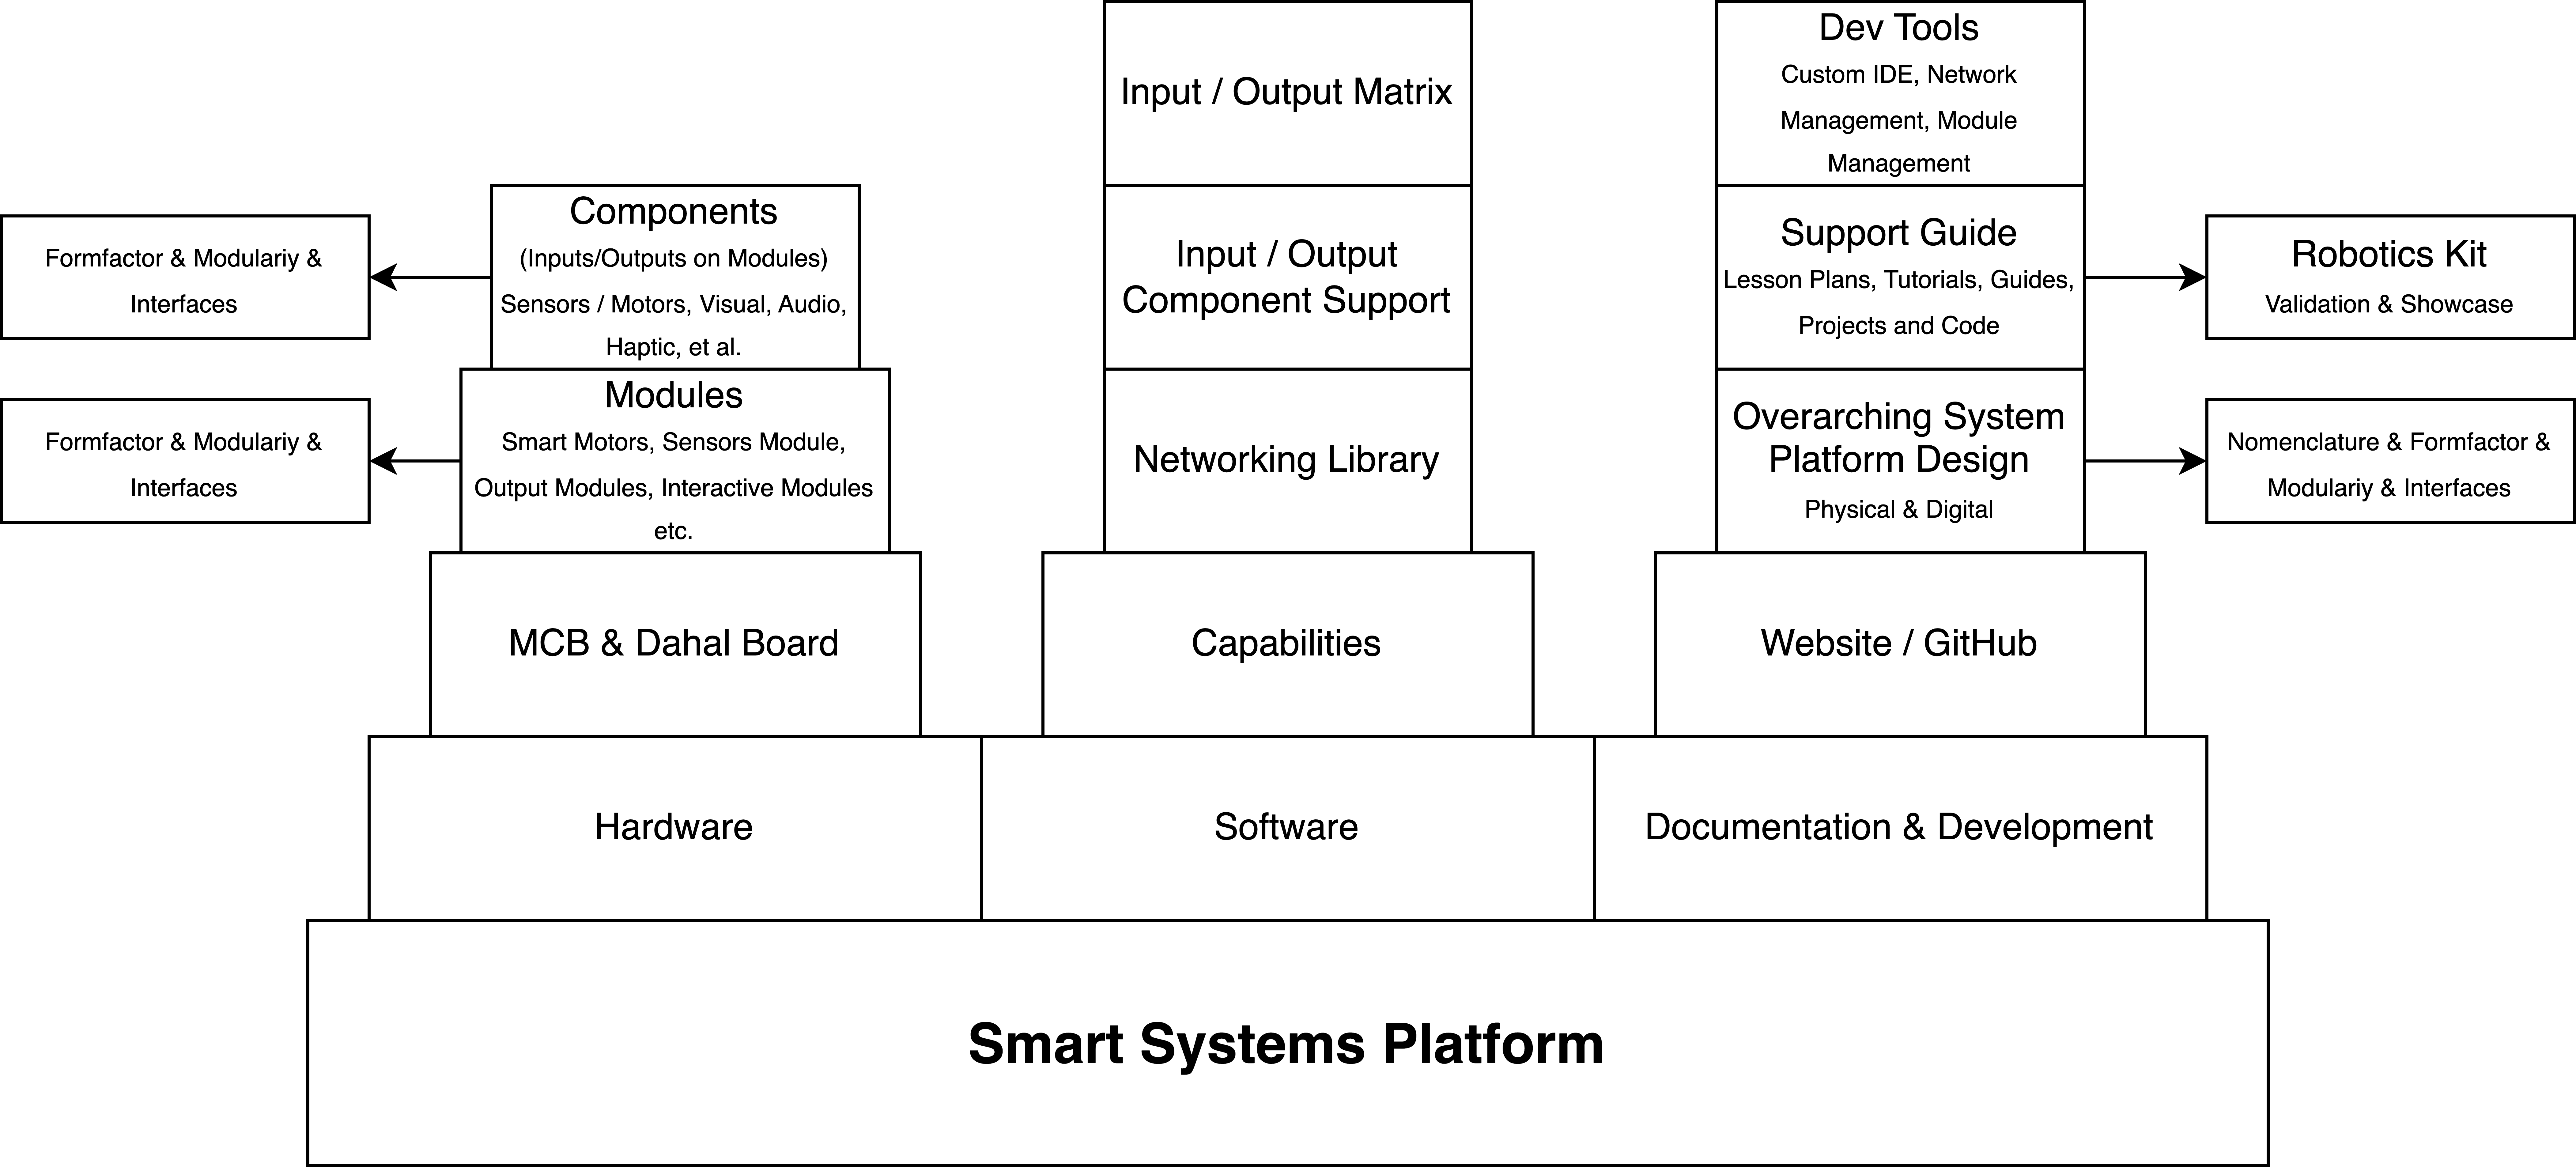
\includegraphics[width=\linewidth]{overleaf/images/Smart Systems Platform.drawio.png}
    \vspace{\ftspace}
    \caption{Platform Architecture}
    \label{fig:met:ssp_architecture}
\end{figure}

The main objective of the platform or framework is to provide access to the developed networking approach and to enable its users, and perhaps in a further step different stakeholders such as educational researchers and educational tool developers or even educators and students, to use the platform, to enable a quick ideation, creation and testing using the provided hardware and capabilities, with no entry barriers.

%\subsubsection{\label{sec:methods_nomenclature}Nomenclature}

In an effort to clarify the concept and the used terms, the SSP-specific nomenclature outlined in Table \ref{tab:nomenclature}.

\begin{table}[H]
    \centering
    \begin{tabular}{|p{125pt}|p{325pt}|}
    \hline
        \textbf{Term} & \textbf{Description} \\\hline
        Hardware        & Physical parts of the Smart System Platform \\\hline
        Module          & Stand alone modules, such as the Smart Motor, also called Smart Modules \\\hline
        Component       & Hardware contained in the module, such as sensors, motors, etc. \\\hline
        Input           & Component that provides data input, such as a sensor \\\hline
        Output          & Component that provides output, such as a motor \\\hline
        UI              & Components that are used to allow user interaction  \\\hline
        Software        & Code files and library saved and running on a Module \\\hline
        Library         & A file to enable a component or capability to work on the module \\\hline
        Networking      & The networking library \\\hline
        SSP Networking  & The SSP-specific networking library add-on library\\\hline
        Firmware        & Firmware running on a Module \\\hline
        Documentation   & Documentation for the Smart System Platform, its modules incl. the website, the development and management tools and the GitHub \\\hline
        Website         & The Website, hosting information and the dev suite, part of documentation \\\hline
        GitHub          & The GitHub page of the Smart System Platform hosting code and all the files \\\hline
        Network Management and Module Configuration Tool & PyScript-based web-application, which allows network management and module control and configuration \\\hline
        Integrated Development Environment & PyScript-based custom web-IDE \\\hline
        Module Management Tool & PyScript-based web-application, which allows modules to be updated to the newest version, based on its configuration \\\hline
        AI Coding Assistant   & ChatGPT-based Large Langue Model (LLM), primed for coding and development assistant using the SSP \\\hline
        AI Module Configuration Assistant & ChatGPT-based LLM, primed for configuring SSP modules for interaction using the Network Management and Module Configuration Tool \\\hline
    \end{tabular}
    \vspace{\ftspace}
    \caption{Nomenclature for the Smart System Platform}
    \label{tab:nomenclature}
\end{table}

%\subsubsection{\label{sec:methods_principles}Guiding Principles}

In line with the principles of the network approach and the ideas outlined in \citet[]{dahal_designing_2024} and section \ref{sec:intro_res_quest} of this thesis, certain guiding principles were used in the design of the platform architecture: 

\begin{itemize}
    \item Simplicity:\\
    The platform was designed to be intuitively understandable, trying to reduce components and parts to a minimum in an effort to lower the learning curve and allow easy access.
    \item Accessibility:\\
    Website, accessibility, information. Free to use, all information publicly available, hosted on GitHub, including website and development tools and guides.
    \item Modularity and Interoperability:\\
    The various components are designed to be modular, interoperable and compatible with each other, both in terms of hardware and software. 
\end{itemize}

\section{\label{sec:methods_ph2}Phase 2: Development}

\subsection{\label{sec:methods_approach}Approach}

An iterative approach has been used in the development of the Networking and the components of the Smart System Platform. Much of the work on the different parts and components has been done in parallel with several interrelated iterations, but for ease of reading the different components are described separately in their own subsections.

\subsection{\label{sec:methods_net_dev}Networking Development}

%Code structure, Commands, Interactions, etc. Message flows, message types, large message handling, IRQ implementation, all commands and handlers Setup with congif, networking and ssp\_networking Boop-o-meter

Given the the requirements and concept for the networking protocol defined in Section \ref{sec:methods_net_des}, the networking library has been split into two parts, the base networking library, which contains the basic networking logic and the more specific SSP networking library, which contains more SSP specific networking logic.

\subsubsection{\label{sec:methods_networking}Base Networking Library}

%\textbf{\label{sec:methods_additional}Additional Considerations}\\\\

The Base Networking Library is a generic, all-purpose, customisable networking library built on top of ESP-NOW protocol, that introduces the basic networking functionality and aims to enhance and exploit the capabilities of ESP-NOW. As outlined in Section \ref{sec:methods_net_des}, ESP-NOW uses MAC addresses to address messages, however, these addresses might not be know beforehand. To this end an address book is included in the networking library, which is automatically populated when a message is sent to a new MAC address or received from an unknown MAC address. In order to be able to discover and gather information about the surrounding modules, the ping command message outlined before, contains information about the sender, such as name and configuration. This ping command can be sent out to the general broadcast address and when received by any device running the networking library, prompts that devices to return a pong message to the sender, which in turn contains information about itself. In this scenario, both devices have now added each other to their respective address books, which includes the mac address, name and configuration. This address book, however, is not persistent and the information is lost upon reboot of the device. In addition, an echo command, which prompts the receiver to return the same message content to the sender, and a boop command, which is intended to calculate and return the stored RSSI values of the last message of every MAC address a message was received from, were also designed as key commands to be included in the base network. Exception catching and handling is included throughout the code to prevent an error in the message transmission or handling process from interrupting the main code. The library also includes time-stamped information, debug and error statement printing in the REPL and logging to a local log.txt file. These three levels of printing and logging can be individually enabled or disabled. Information print statements are placed only when necessary, such as when sending or receiving, while debug logs are placed in every function and additionally at every critical point in the code, and error logs are logs of caught exceptions.\\

\textbf{\label{sec:methods_msg_struct}Message Structure}\\\\
The message structure developed for the networking library is shown in Table \ref{tab:msg_struct}. The message starts with a header ($0x2a$, 1 byte) which is used to identify that the message has been sent by a friendly networking library. 
This is followed by the message type, which currently identifies the message as one of the three different message types ($0x01$ for \textit{cmd}, $0x02$ for \textit{inf} and $0x03$ for \textit{ack}, $1\ byte$) defined in Section \ref{sec:methods_net_des}. 
The type is followed by the message subtype, which identifies the specific subtype of the message (\textit{cmd}: $0x10$ for \textit{ping}, $0x13$ for \textit{boop} and $0x15$ for \textit{echo}; \textit{inf}: $0x20$ for \textit{boop response}, $0x21$ for \textit{data} and $0x22$ for \textit{message}; \textit{ack}: $0x10$ for \textit{pong} and $0x15$ for \textit{echo}), although only a few subtypes are defined in the basic network. However, the library has provisions to allow the user to define their own message subtypes and their respective handling logic, as is done in the more application specific SSP networking library.
The timestamp is populated at the time of sending with \verb!time.ticks\_ms\end!, which is the time in milliseconds since the device was started. \verb!time.ticks\_ms! returns a $32-bit$ unsigned integer, ensuring that it always stays under $4\ bytes$ by rolling over when it reaches its maximum value. In the case of a $32-bit$ integer, the maximum would be $2^{32} -1\ ms = 4'294'967^295\ ms = 49.71\ days$. However, according to the MicroPython documentation \citep{micropython_micropython_2025-2}, the exact maximum size of \verb!time.ticks\_ms\! in MicroPython is opaque, although in the case of the MicroPython implementation for ESP32s, the maximum size appears to be only 30 bits, resulting in a maximum of $2^{30}-1\ ms=1'073'741'823\ ms = 12.43\ days$.
As such, the timestamp is only used to calculate relative durations or differences, for example in the ping command, where the timestamp is returned to the original sender, who then calculates the ping time, the time it took for the message to travel back and forth.
The data type field is used to identify the encoding of the payload, as the network code allows the following data types to be encoded: \textit{integer}, \textit{string}, \textit{float}, \textit{list}, \textit{dictionary}, \textit{bytes} and \textit{bytearray}. In addition, the data type is also used to identify long messages, i.e. when a payload longer than $241\ bytes$ is split and sent using multiple messages. In this case the payload type is set to the long message code, where the payload contains its own structure, namely the part number of the message, the total number of parts of the long message and the payload type of the message. Taking into account these three additional meta-informations, each of which occupies one byte per message, the remaining payload is $238\ bytes$. With one byte allocated to the part number of the message, the maximum number of parts is $256$ as the part number is stored in $1\ byte$, giving a theoretical payload limit of $256*238\ bytes = 60'928\ bytes$. The logic of long message handling is further defined in Section \ref{fig:net_recv_logic}. With eight options, the data type field is ($1\ byte$).
This is followed by the data field containing the payload. This payload is encoded depending on the type of data, with the field holding a maximum of $241\ bytes$.
Finally, the message structure contains a $1\ byte$ checksum to confirm the integrity of the message. The checksum is calculated by taking the sum of all the preceding fields and calculating the modulus of the sums divided by $256$, ensuring a number smaller than $256$ and therefore fitting into the $1\ byte$ space allocated to it. 
However, the message structure does not include the sender's MAC address, as this is already passed by ESP-NOW and included in the surrounding Wi-Fi management frame.

%in the message structure (250 bytes - 9 bytes, which are used for identifier, types, subtypes, send time payload type and the checksum). This is achieved by splitting the data into multiple messages, up to 256 parts, resulting in a total theoretical maximum payload of 60'928 bytes (256 x 238 bytes). The payload is reduced to 238 bytes because 3 additional variables are used to identify the message, the payload type to identify a long message, the actual payload type, the total number of messages and the current message number.

\begin{table}[H]
    \centering
    \begin{tabular}{|c|c|c|c|c|c|c|}
        \hline
        Header & Type & Sub-Type  & Timestamp & Data Type & Data & Checksum \\
        ($1\ byte$) & ($1\ byte$) & ($1\ byte$) & ($4\ bytes$) & ($1\ byte$) & ($241\ bytes$) & ($1\ byte$) \\
        \hline
        Identifier & Number & Number & Number & Number & \textbf{Payload} & Number \\
        0x2a & (1-3) & (0-255) & $time.ticks\_ms()$ & (0-6) & ... & $sum() \% 256$ \\
        \hline
    \end{tabular}
    \vspace{\ftspace}
    \caption{Networking Message Structure}
    \label{tab:msg_struct}
\end{table}

\subsubsection{\label{sec:methods_send_logic}Send Logic}

The send logic of the Networking Library is outlined in Figure \ref{fig:net_send_logic}. The structure is similar to a funnel, with the pipeline able to be called in a number of ways, either by directly calling one of the implemented command functions, which will format the content and send the appropriate cmd or info type message, such as the ping, echo and boop commands, as well as normal message or data type messages. There is also a command to send custom type of msg, which requires the message type and message subtype to be specified. These functions can be called manually by users or by code using the library, although there are some other internal functions, which start the send pipeline, which can only be automatically called from within the network code. This is the case for sending most ack message types such as pong, confirmation, success or fail. The various functions for sending specific command types contain logic to look up the appropriate code and format the payload as required by the custom handling logic, and then call the custom send command in the network. Depending on the specific commands, different inputs are required, at least the mac address or a list of mac addresses if the message needs no content, as in the case of ping, or the mac and the message or data, as in the case of message or data type messages. And as mentioned above, the type and subtype are also required for the custom send commands. These functions then call the compose function, which attempts to encode the content into payloads. After encoding the content into the payload, the code checks the length of the payload and, if necessary, splits the message into several parts to ensure a size of $250\ bytes$ or less for each message. The payload is then structured into the message or messages according to the msg structure. To avoid confusion with the message type of the same name, these encoded messages are referred to only as msg. The code then loops through the list of macs, attempts to add them to the ESP-NOW buffer, then loops through all the msgs and attempts to send each corresponding message. This function will attempt to resend the message three times if an error occurs or if a receipt is not received from the recipient. After sending, the corresponding mac address is immediately removed from the ESP-NOW buffer to avoid a buffer overflow and to circumvent the 20 peer limit imposed by ESP-NOW. Exception handling is included throughout the code to prevent an error in the sending process from interrupting the main code, including but not limited to catching invalid mac addresses, invalid message content, or when interfacing with the ESP-NOW library.

\begin{figure}[H]
    \centering
    \includegraphics[width=\linewidth]{overleaf/images/send_logic.drawio.png}
    \vspace{\ftspace}
    \caption{Networking Message Send Logic}
    \label{fig:net_send_logic}
\end{figure}

\subsubsection{\label{sec:methods_recv_logic}Receive Logic}

The receive logic of the networking library is more complex than the send pipeline. It starts as a linear pipeline since the function to start it, can only be called by a interrupt request (IRQ) of ESP-NOW, which is called when ESP-NOW has received a new msg. The logic follows a tree shape and splits into many different branches to handle the different message types, as shown in Figure \ref{fig:net_recv_logic}. \\
The first step is for the ESP32 to receive a msg which, after some magic, is handled by ESP-NOW. ESP-NOW then calls the IRQ function, which in our case checks if there is a msg in the ESP-NOW buffer, and then calls the receive function. The receive function loops and gets msg and sender mac from the ESP-NOW msg buffer as long as there are msgs in the ESP-NOW msg buffer. For each msg it receives, it calls the process function, which attempts to add the sender's mac address to the network address book. It then calls the decode function which tries to split the msg according to its structure. If the msg has the wrong structure, does not start with our identifier, or the checksum is incorrect, the msg is discarded. If the msg is split successfully, the payload type is checked, and if the payload type indicates a long message, the msg is sent to the long msg handlers, which decode the payload, collect its number, the total part of msgs and the actual payload type, and add it to the payload buffer. If the payload buffer now contains all parts of the msg, the payload is assembled and passed on. There it attempts to decode the message according to the data type specified by the payload type variable. It is then passed to the handler function, which sorts the msg by type, passes it to the appropriate handler, sorts it by subtype, and calls the appropriate code or logic. In the case of a ping cmd msg, this will result in a pong ack msg being sent back to the sender. In the case of a message or data type msg, the content is added to the message or data buffer, while ack msg types usually do nothing with the message, except in the case of the pong msg, the information encoded in the content of the msg is used to add further information about the peer to the networking library address book. If the subtype of the message is not found, the custom subtype handler, if set, is called, where custom handlers are checked. This is the case for the additional SSP networking library, which defines a number of additional msg subtypes and their respective handling. In any case, any received msg that ahs made it to the handler will be logged as level information. Finally, custom IRQ functions can be called for different message types, if set, and a general custom IRQ function is called after all messages in the ESP-NOW msg buffer have been processed. \\
Exception handling is included throughout the code to prevent an error in the sending process from interrupting the main code, including but not limited to catching msgs with an invalid structure, msgs with an invalid payload encoding, or invalid content in terms of handling logic, or any errors that may occur when interfacing with the ESP-NOW library.

\begin{figure}[H]
    \centering
    \includegraphics[width=\linewidth]{overleaf/images/receive_logic.drawio.png}
    \vspace{\ftspace}
    \caption{Networking Message Receive Logic}
    \label{fig:net_recv_logic}
\end{figure}

%\textbf{\label{sec:methods_additional}Additional Considerations}\\\\

\subsubsection{\label{sec:methods_ssp_networking}SSP Networking}

Building on the base networking library and using the designed interfaces, the SSP specific networking add-on has been designed, which defines a variety of SSP specific commands and message types and subtypes, as well as the corresponding custom command handlers for use with different Smart Modules for different applications. The SSP networking library is specifically designed to work with Smart Motors and other Smart Modules and requires both the base networking.py and a smart module config.py configuration file to properly function, as shown in the Figure \ref{fig:net_code_structure}.

\begin{figure}[H]
    \centering
    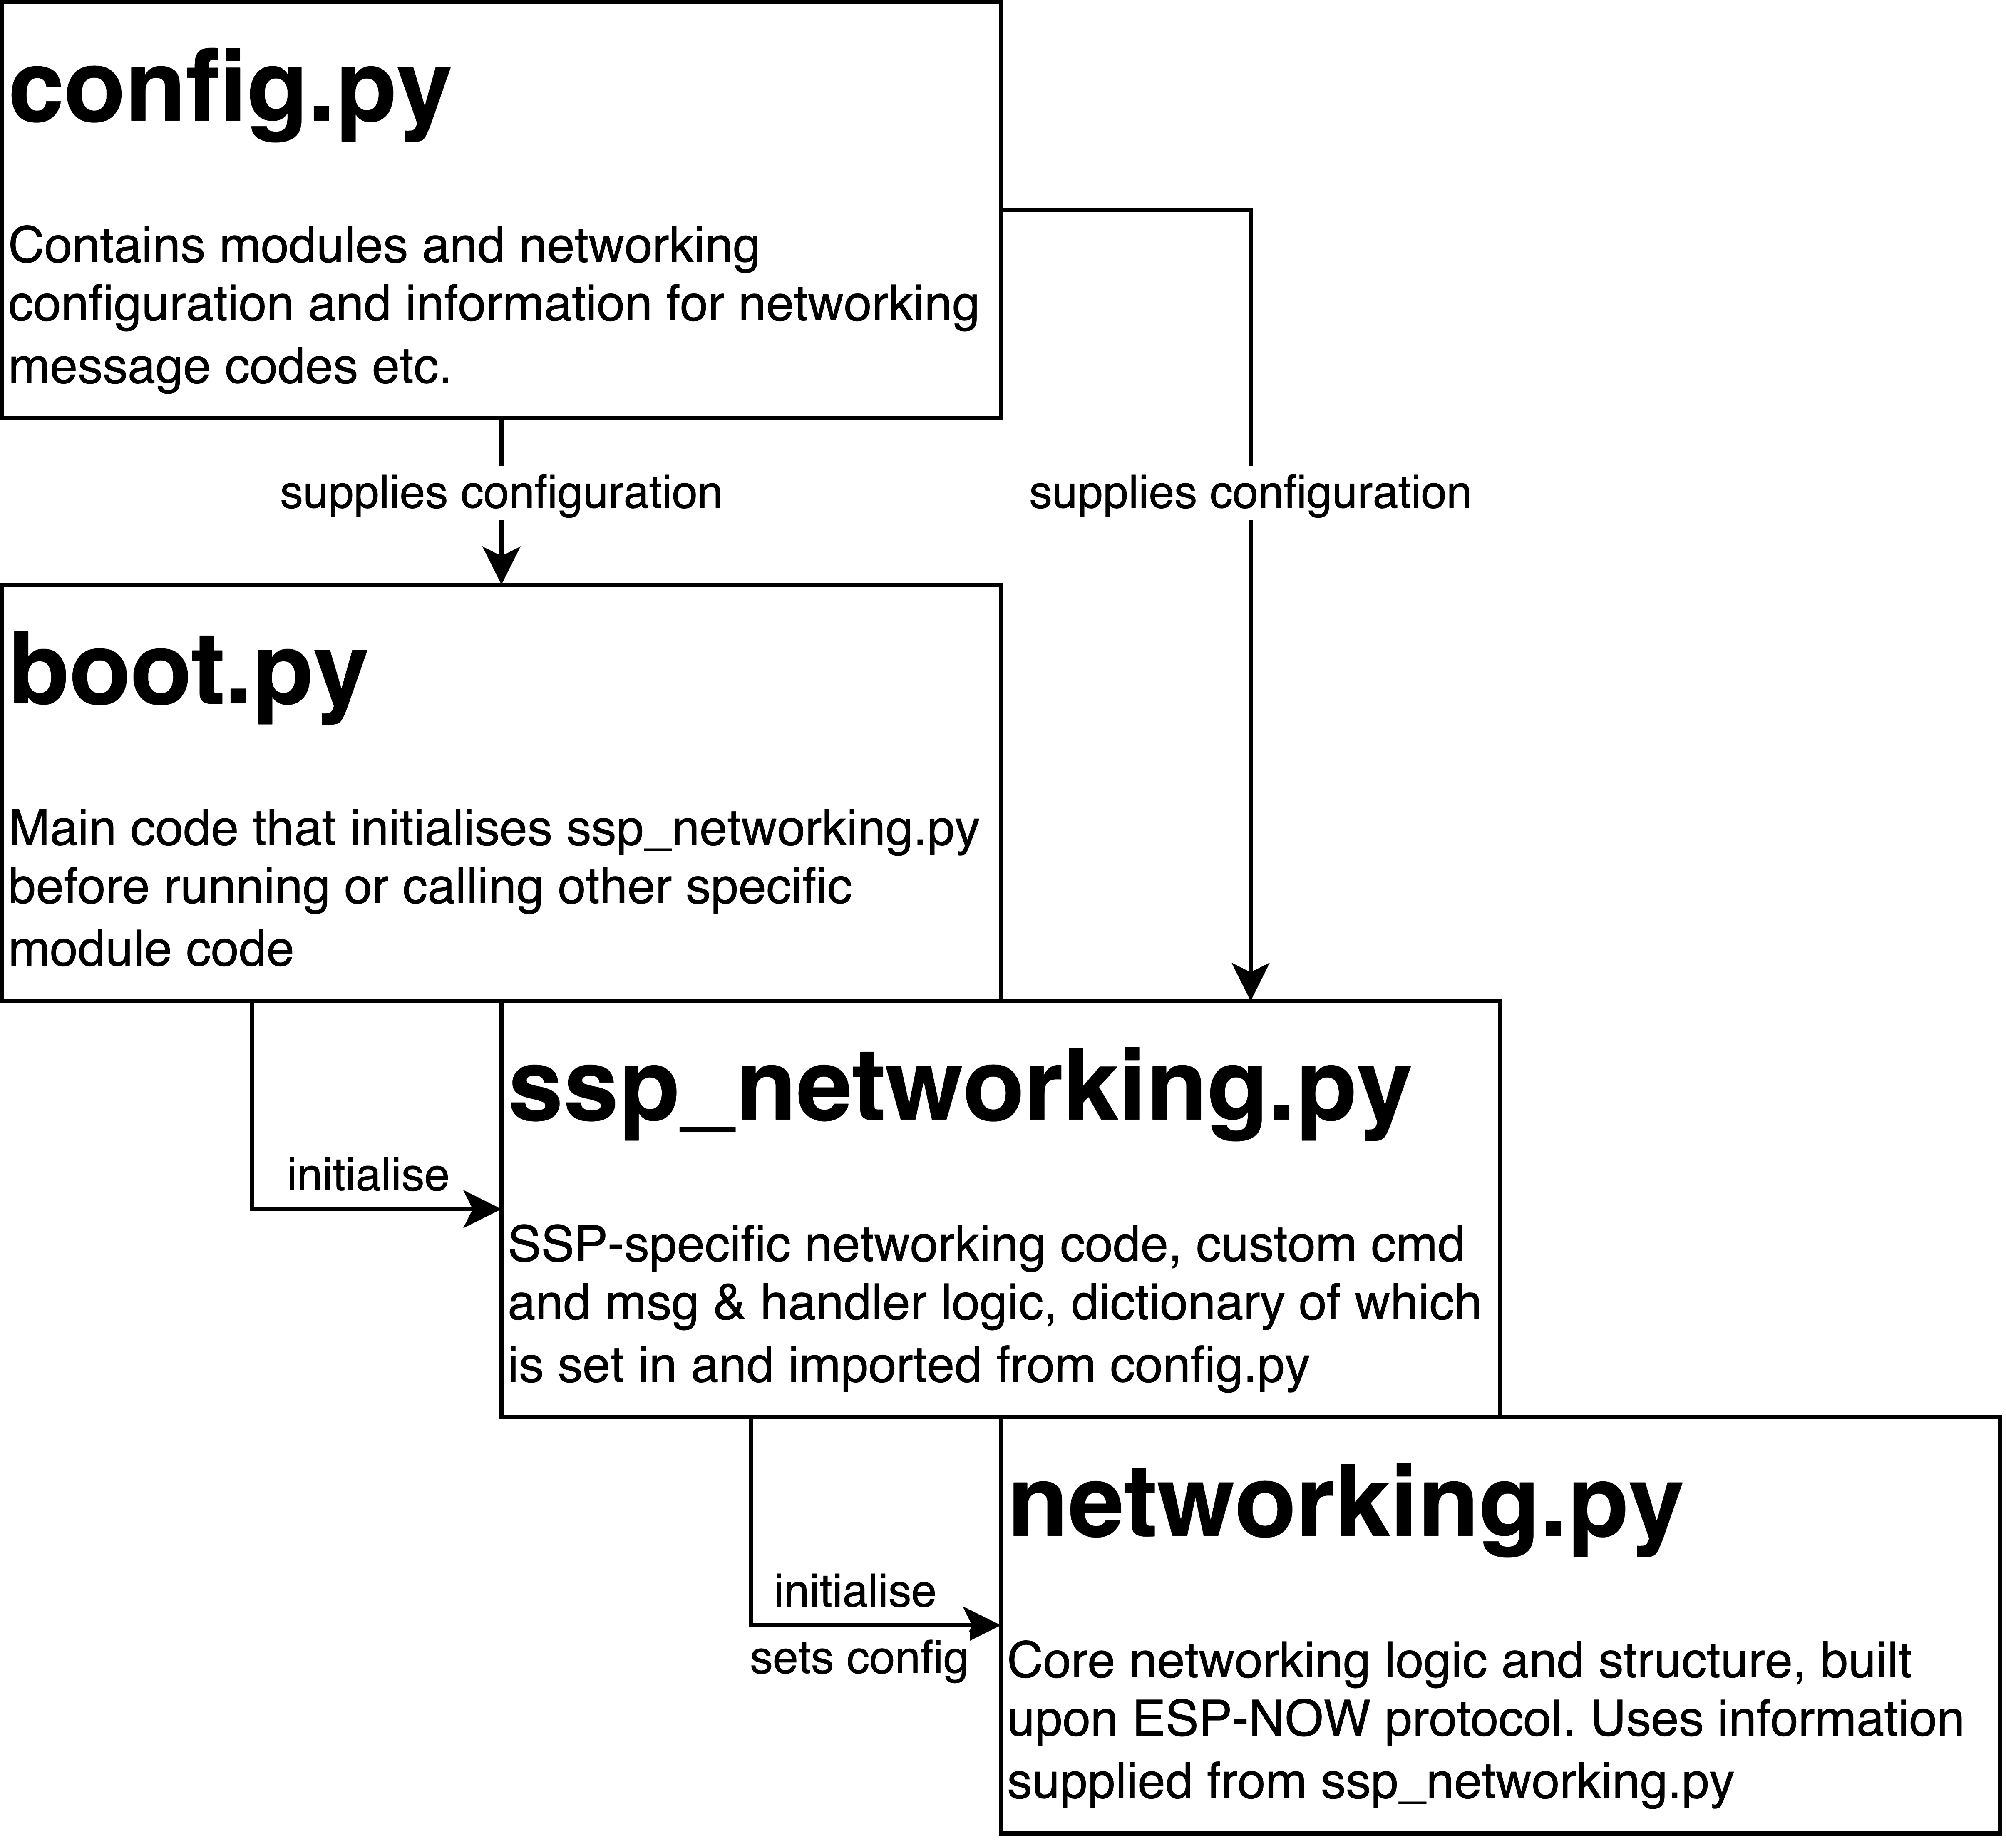
\includegraphics[width=.6\linewidth]{overleaf/images/code_structure.png}
    \vspace{\ftspace}
    \caption{Networking Code Structure}
    \label{fig:net_code_structure}
\end{figure}

With the aim of future-proofing the code design and making it easy to use the code provided for future projects, SSP Networking has been designed with a variety of applications and functionalities in mind, which is reflected in the large number of custom commands and message types. Figure \ref{fig:net_net_structure} shows the detailed class and function structure of the two libraries, which illustrates the variety of custom send commands available in the SSP Networking add-on. These include all the basic networking commands and some variations thereof, which are made accessible in the SSP Networking add-on, but call the underlying basic networking functions. In addition, the add-on includes commands such as reboot, commands to configure modules to interact, download files, enable AP, connect to Wi-Fi, get the MCBs file directory, change the configuration or configuration file of another module and so on. It also includes an authentication check that only executes certain commands from admin modules whose MAC address is in the configuration's whitelist, or which use a sudo bypass\footnote{This can be achieved by adding the string "sudo" to a payload list at position [-1].}. The handling of all the custom commands isn't split into different functions, but is contained within the three specific custom type handlers.

\begin{figure}[H]
	\centering%
    \begin{subfigure}[b]{0.45\textwidth}%
      	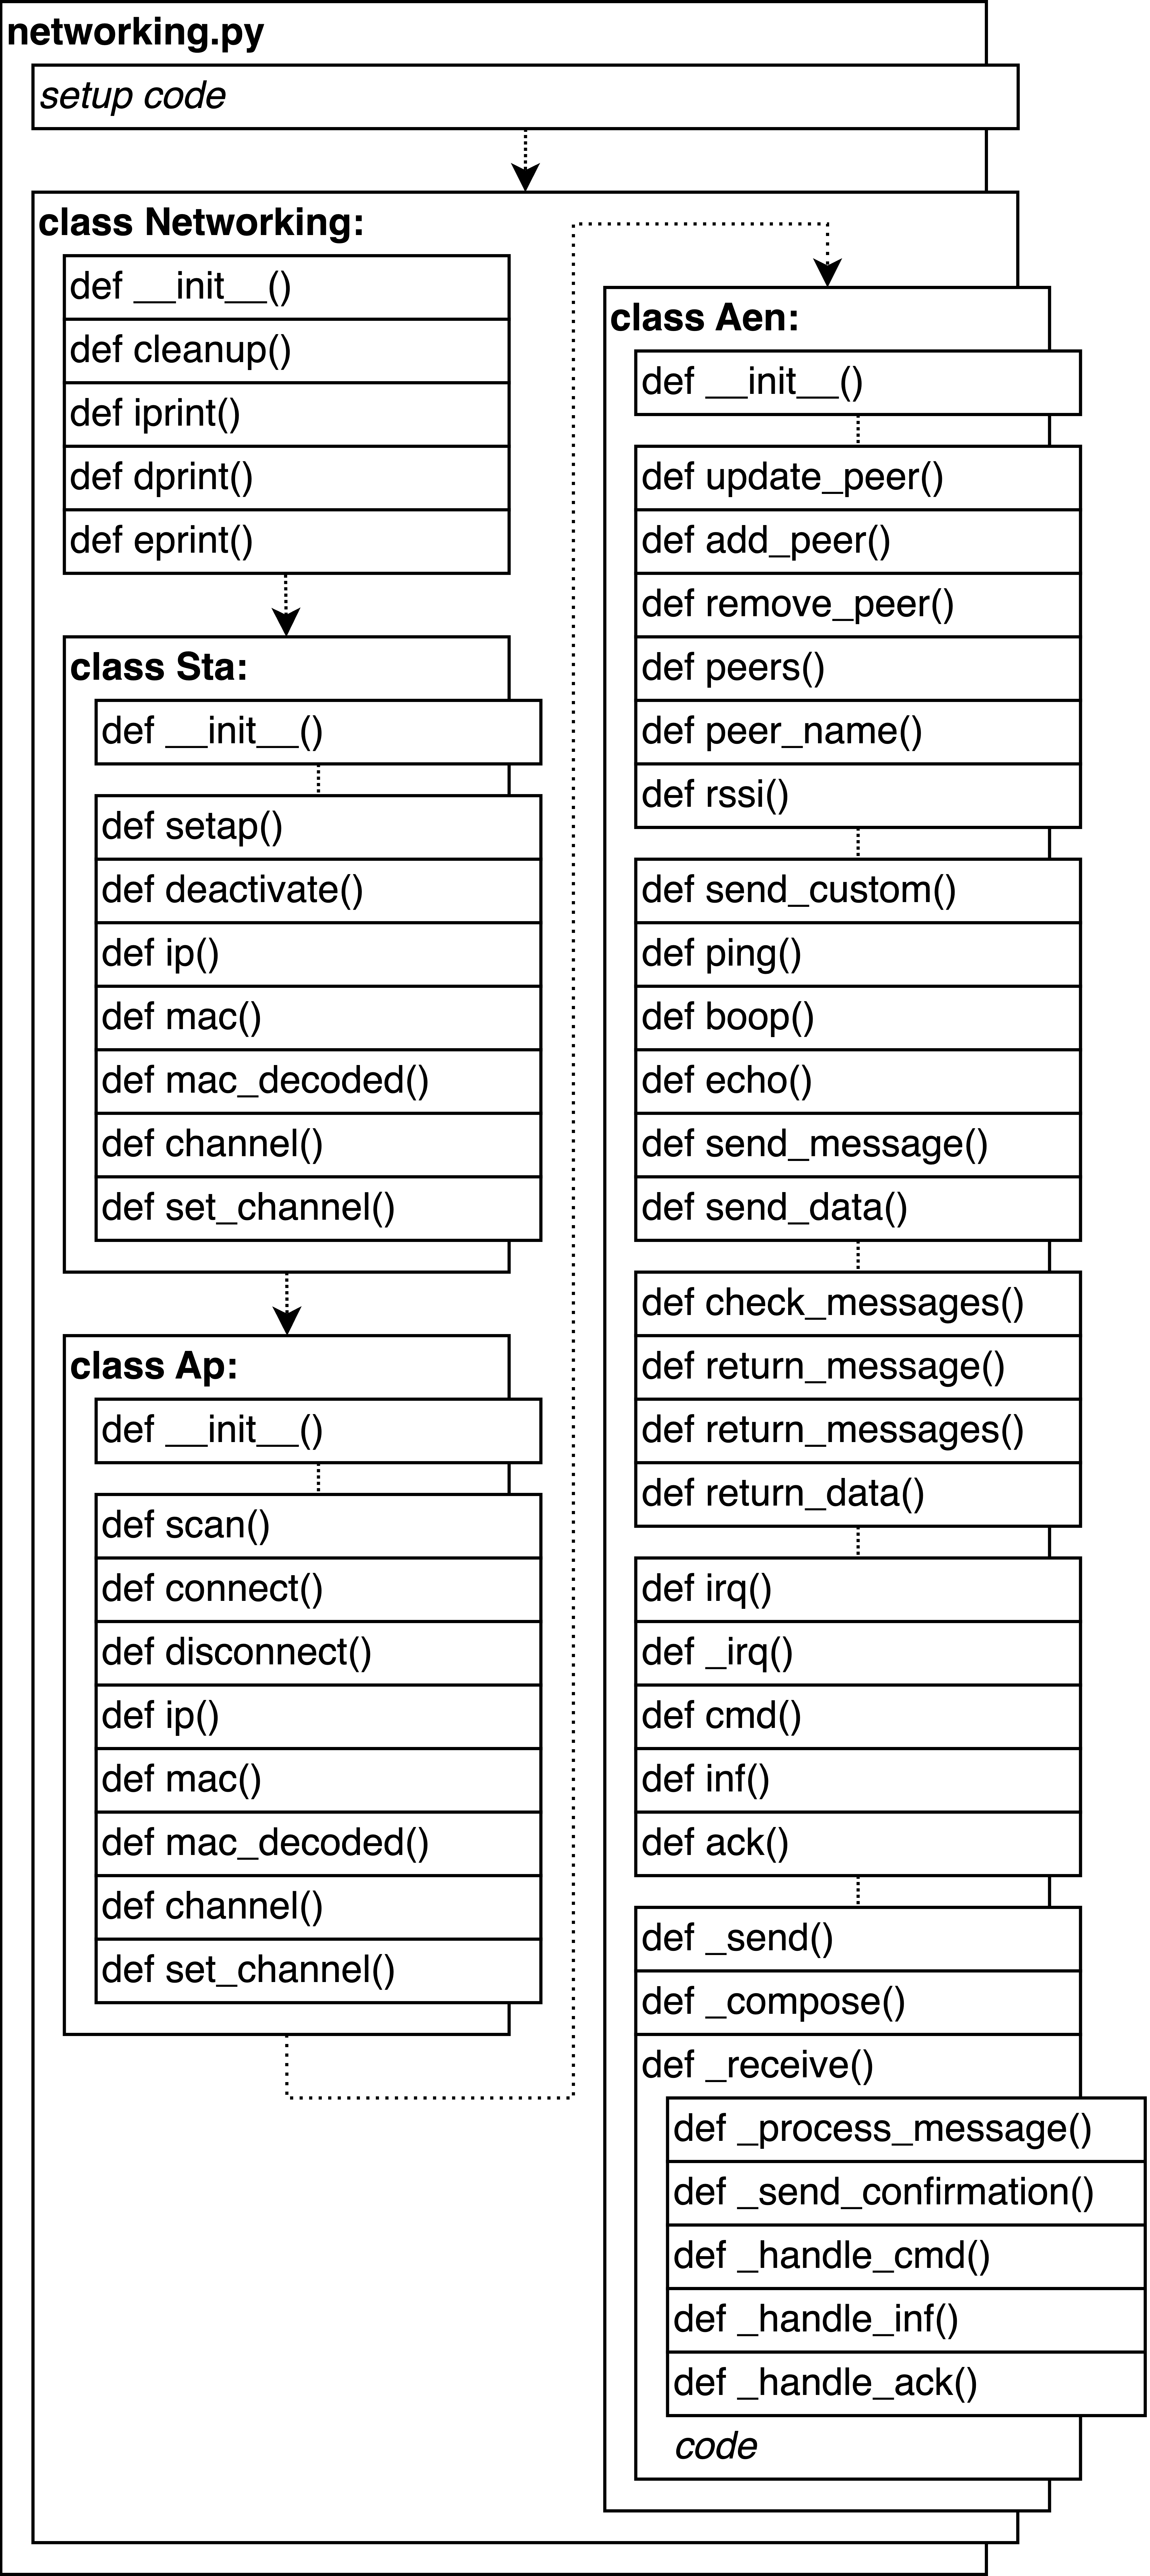
\includegraphics[width=\textwidth]{overleaf/images/networking_structure.drawio.png}%
    \end{subfigure}%
    \hspace{0.05\textwidth}
    \begin{subfigure}[b]{0.45\textwidth}%
        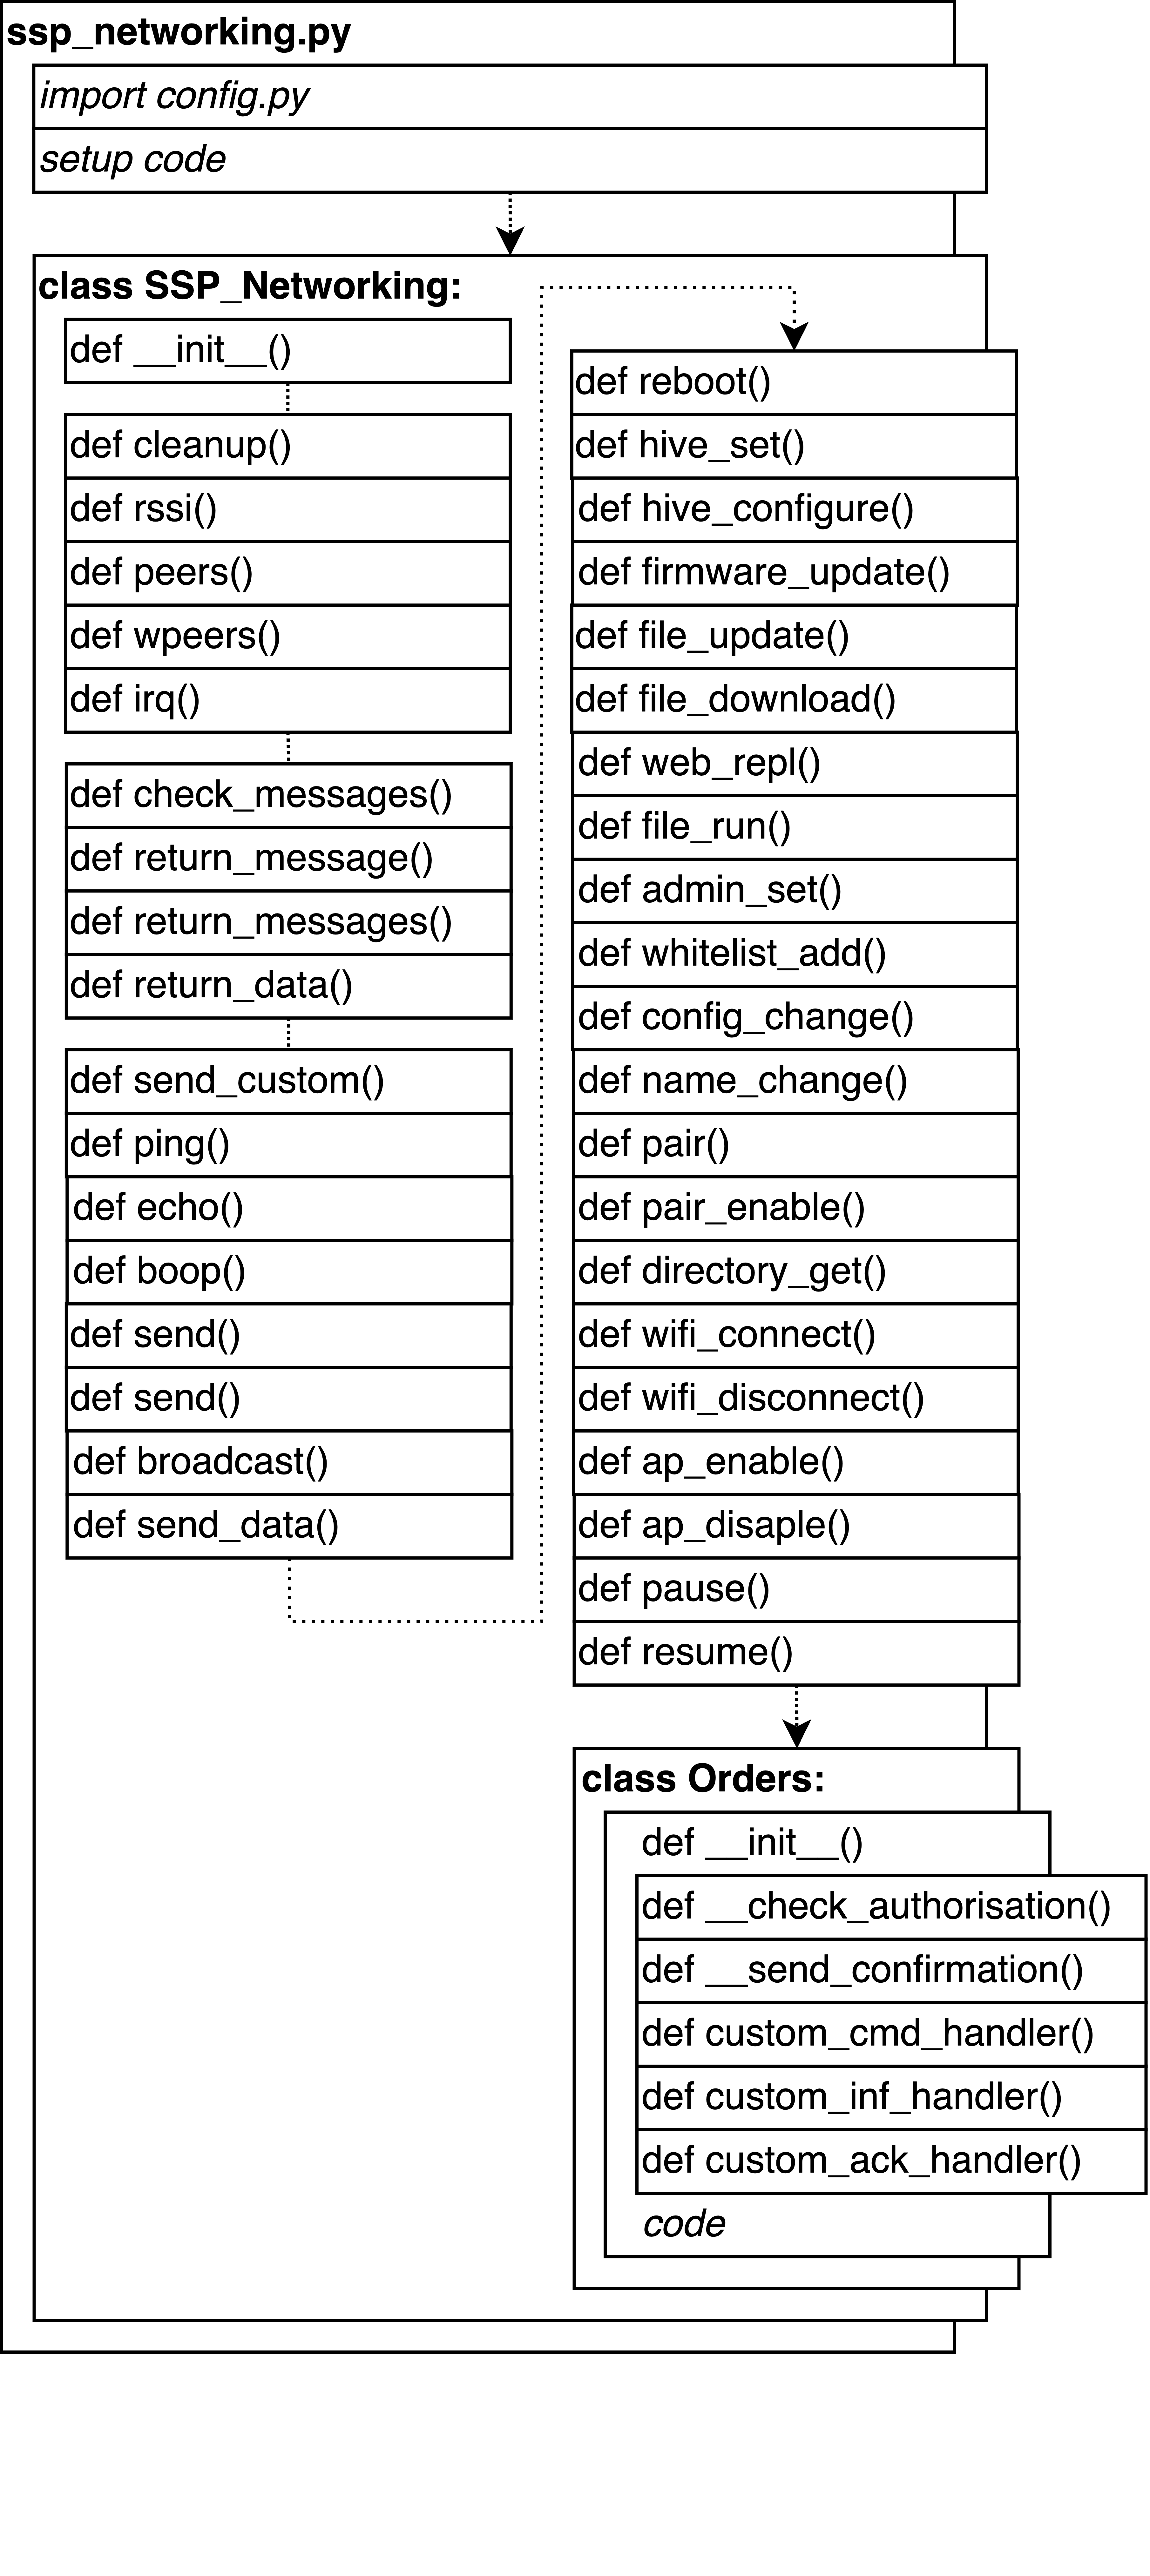
\includegraphics[width=\textwidth]{overleaf/images/ssp_networking_structure.drawio.png}%
    \end{subfigure}%
    \vspace{\ftspace}
    \caption{networking.py and ssp\_networking.py code structure}
    \label{fig:net_net_structure}
\end{figure}

\subsection{\label{sec:methods_ssp_dev}Smart System Platform Development}

In addition to the concept and design of the Smart System Platform, described in Section \ref{sec:methods_ssp_des}, several components have been developed, which are described in this section. These include parts of the documentation, such as the GitHub page and the website, including the various networking development and management tools developed in PyScript that are part of the website.

\subsubsection{\label{sec:methods_gh}GitHub}
As part of the software development, a public GitHub page has been created for this thesis to host the code and development progress for the network. However, in line with the goal of accessibility, the public GitHub page also serves as the main host for all other information and resources of the Smart System Platform, including the website, all data related to this thesis, and more, with the exception of PyScript. The site is licensed under the MIT licence. 

In terms of organisation, the page is divided into SSP folders, namely docs, which contains the website files, firmware, which contains the firmware files, hardware, which contains the hardware related files and software, which contains the code. There are also thesis-specific folders, overleaf, which host the thesis report, and RStudio, which hosts the draft automated README files and any experimental data that has been analysed. The GitHub is connected to overleaf and RStudio to allow for automatic . There are also two hidden folders, .github, which hosts the custom GitHub workflows, and the .git folder, which hosts git-specific files.

The main branch of GitHub is restricted and protected, preventing direct commits to it, requiring a pull request that must be approved before merging. Active development takes place in subversions of the /dev branch. Development done by the author is hosted in the dev/nick branch. This was done in an effort to protect the main release versions of the code from accidental editing.

\begin{figure}[H]
    \centering
    
\includegraphics[width=0.5\linewidth]{overleaf/images/placeholder.png}
    \vspace{\ftspace}
    \caption{GitHub Workflow, Branches and Automation}
    \label{fig:enter-label}
\end{figure}

To help with the development workflow, some automation has been introduced on GitHub. Automated activities include the building of the website, which is automated and triggered whenever there is a push or merge to the main branch. In addition to the website being built, there is a custom render and release pipeline that is triggered by merge commits. As the main branch is restricted and can't be committed to directly, it requires a pull request to be submitted and approved. The pipeline is triggered when the pull request is approved and merged. It then automatically populates the software/release folder with all relevant code files from their various locations, and updates config.py with the version of those files. The pipeline then renders all the Quarto Markdown README files, updating them to include the latest file structure and information about the respective folders and their files. Finally, the pipeline merges the above changes back into the branch from which the pull request originated.

\begin{figure}[H]
    \centering
    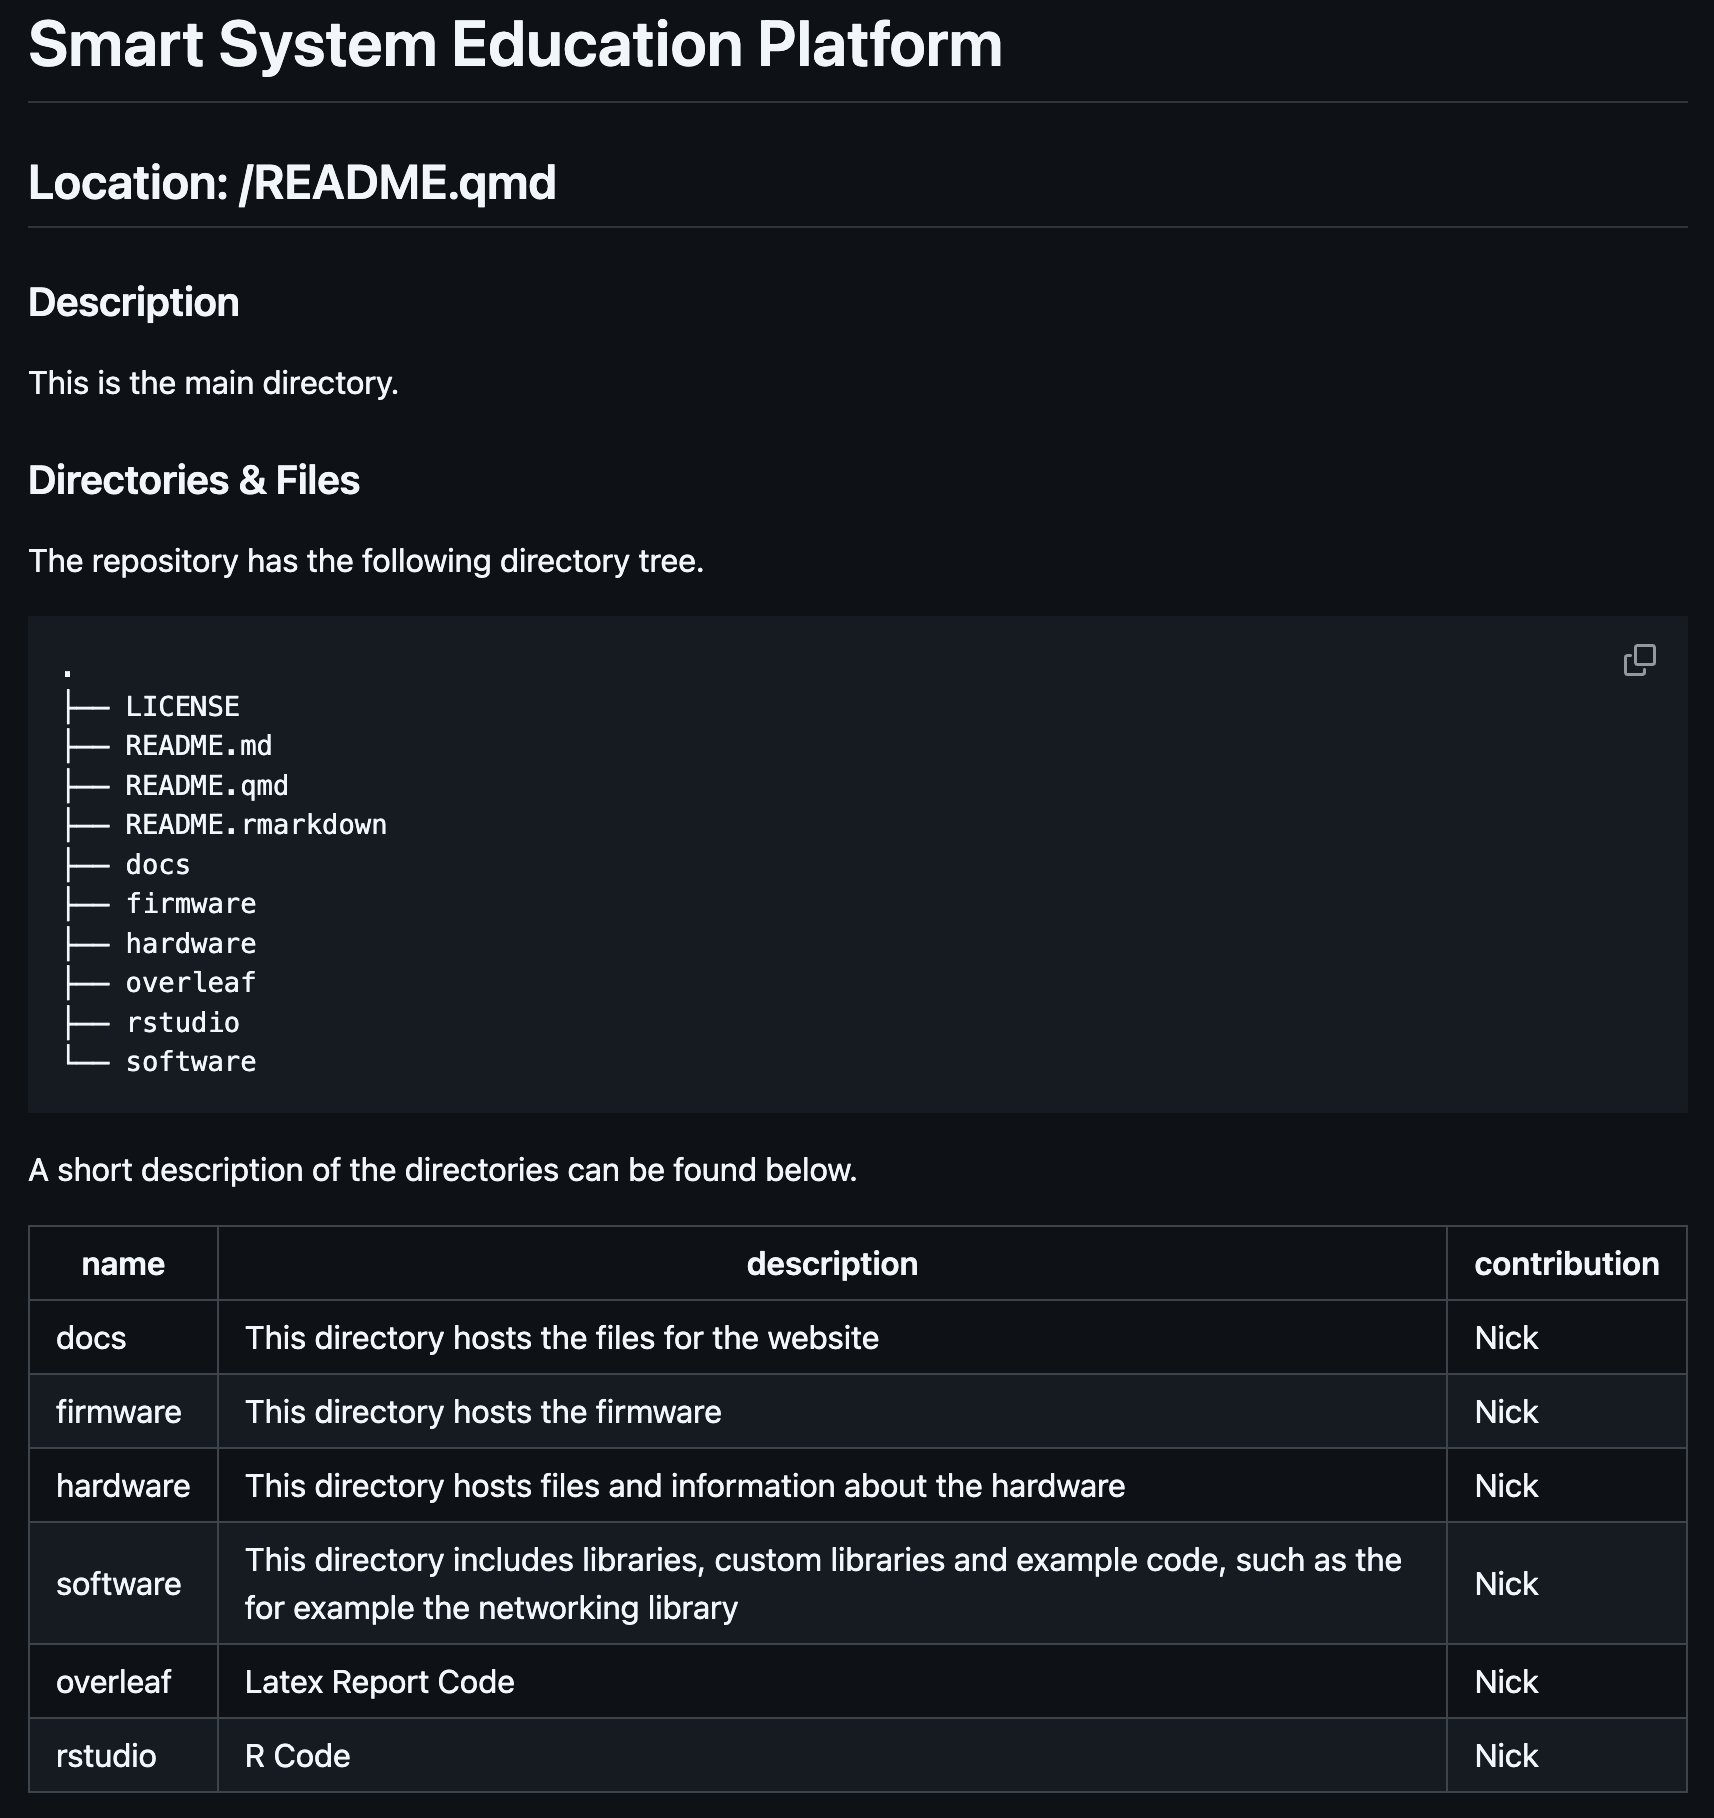
\includegraphics[width=0.5\linewidth]{overleaf/images/readme.png}
    \vspace{\ftspace}
    \caption{Example of the README.md file, which is used to give information about the current directory and its files}
    \vspace{\ftspace}
    \label{fig:readme}
\end{figure}

\subsubsection{\label{sec:methods_pyscript}Development and Management Tools}

In an effort to facilitate interaction with the developed network library and for the sake of accessibility, various tools have been created to assist in the management and development using the Smart System Platform.\\

\textbf{\label{sec:methods_ide}Integrated Development Environment}\\

A read-eval-print loop (REPL) is a simple, interactive interface to a computing device, in the case of MCs using asynchronous serial communication with a universal asynchronous receiver/transmitter (UART). It provides outputs, can accept user input, execute supplied code and return results to the user. A REPL is also the area where print statements are displayed from code running on a device. The MicroPython REPL prompt is provided by default on the device's serial peripheral UART0, connected to pins GPIO1 for TX and GPIO3 for RX, with a baud rate of 115200. \citep{micropython_micropython_2025} The ESP32C3 MCB also has a USB-to-serial converter that allows direct connection to the REPL via the USB interface. This allows connections to be made directly from an IDE such as Thonny or PyCharm. However, Chrome-based browsers also allow websites to connect to devices via various serial ports, such as USB, which was used by \citet{webreflection_micro-repl_nodate} to build micro-repl, a web-based REPL, which was used by \citet[]{rogers_serial_nodate} to build a web-based IDE using PyScript. The advantage of a web-based IDE is that it requires no software installation and works out of the box in the Chrome browser. This web-based IDE was used as the basis for the development of the custom SSP IDE, specifically designed and specified for use with the Smart System Platform and Networking Library, which was developed using PyScript. PyScript is an open source platform for Python in web-browser, aimed to enable development of web-applications using Python. \citep{anaconda_inc_pyscript_2025,anaconda_inc_pyscript_nodate,anaconda_inc_pyscriptnet_nodate}\\

The REPL area, which represents the connected module, includes a REPL area where the serial REPL is displayed. It also contains REPL and SSP specific command buttons such as a button to connect to a module, ctrl-c and ctl-d, clear repl and an export button to export the complete REPL text to a local file. The SSP specific module commands are reinitialise, which initialises a base code, which initialises networking, ping, which sends a ping command message, echo, which sends an echo message, message, which sends a message type msg and rssi, which prints the RSSI table of the module. 
The code stage area, which represents the website/computer side, includes a space for writing code, as well as various command buttons for uploading code files whose contents are then displayed in the stage area, an upload button that uploads the code in the stage area as a file to the module, a selection menu and a view button to display code from code files from the device, a save to PC button to save the selected file to PC and a delete button to delete the selected file.

\begin{figure}[H]
    \centering
    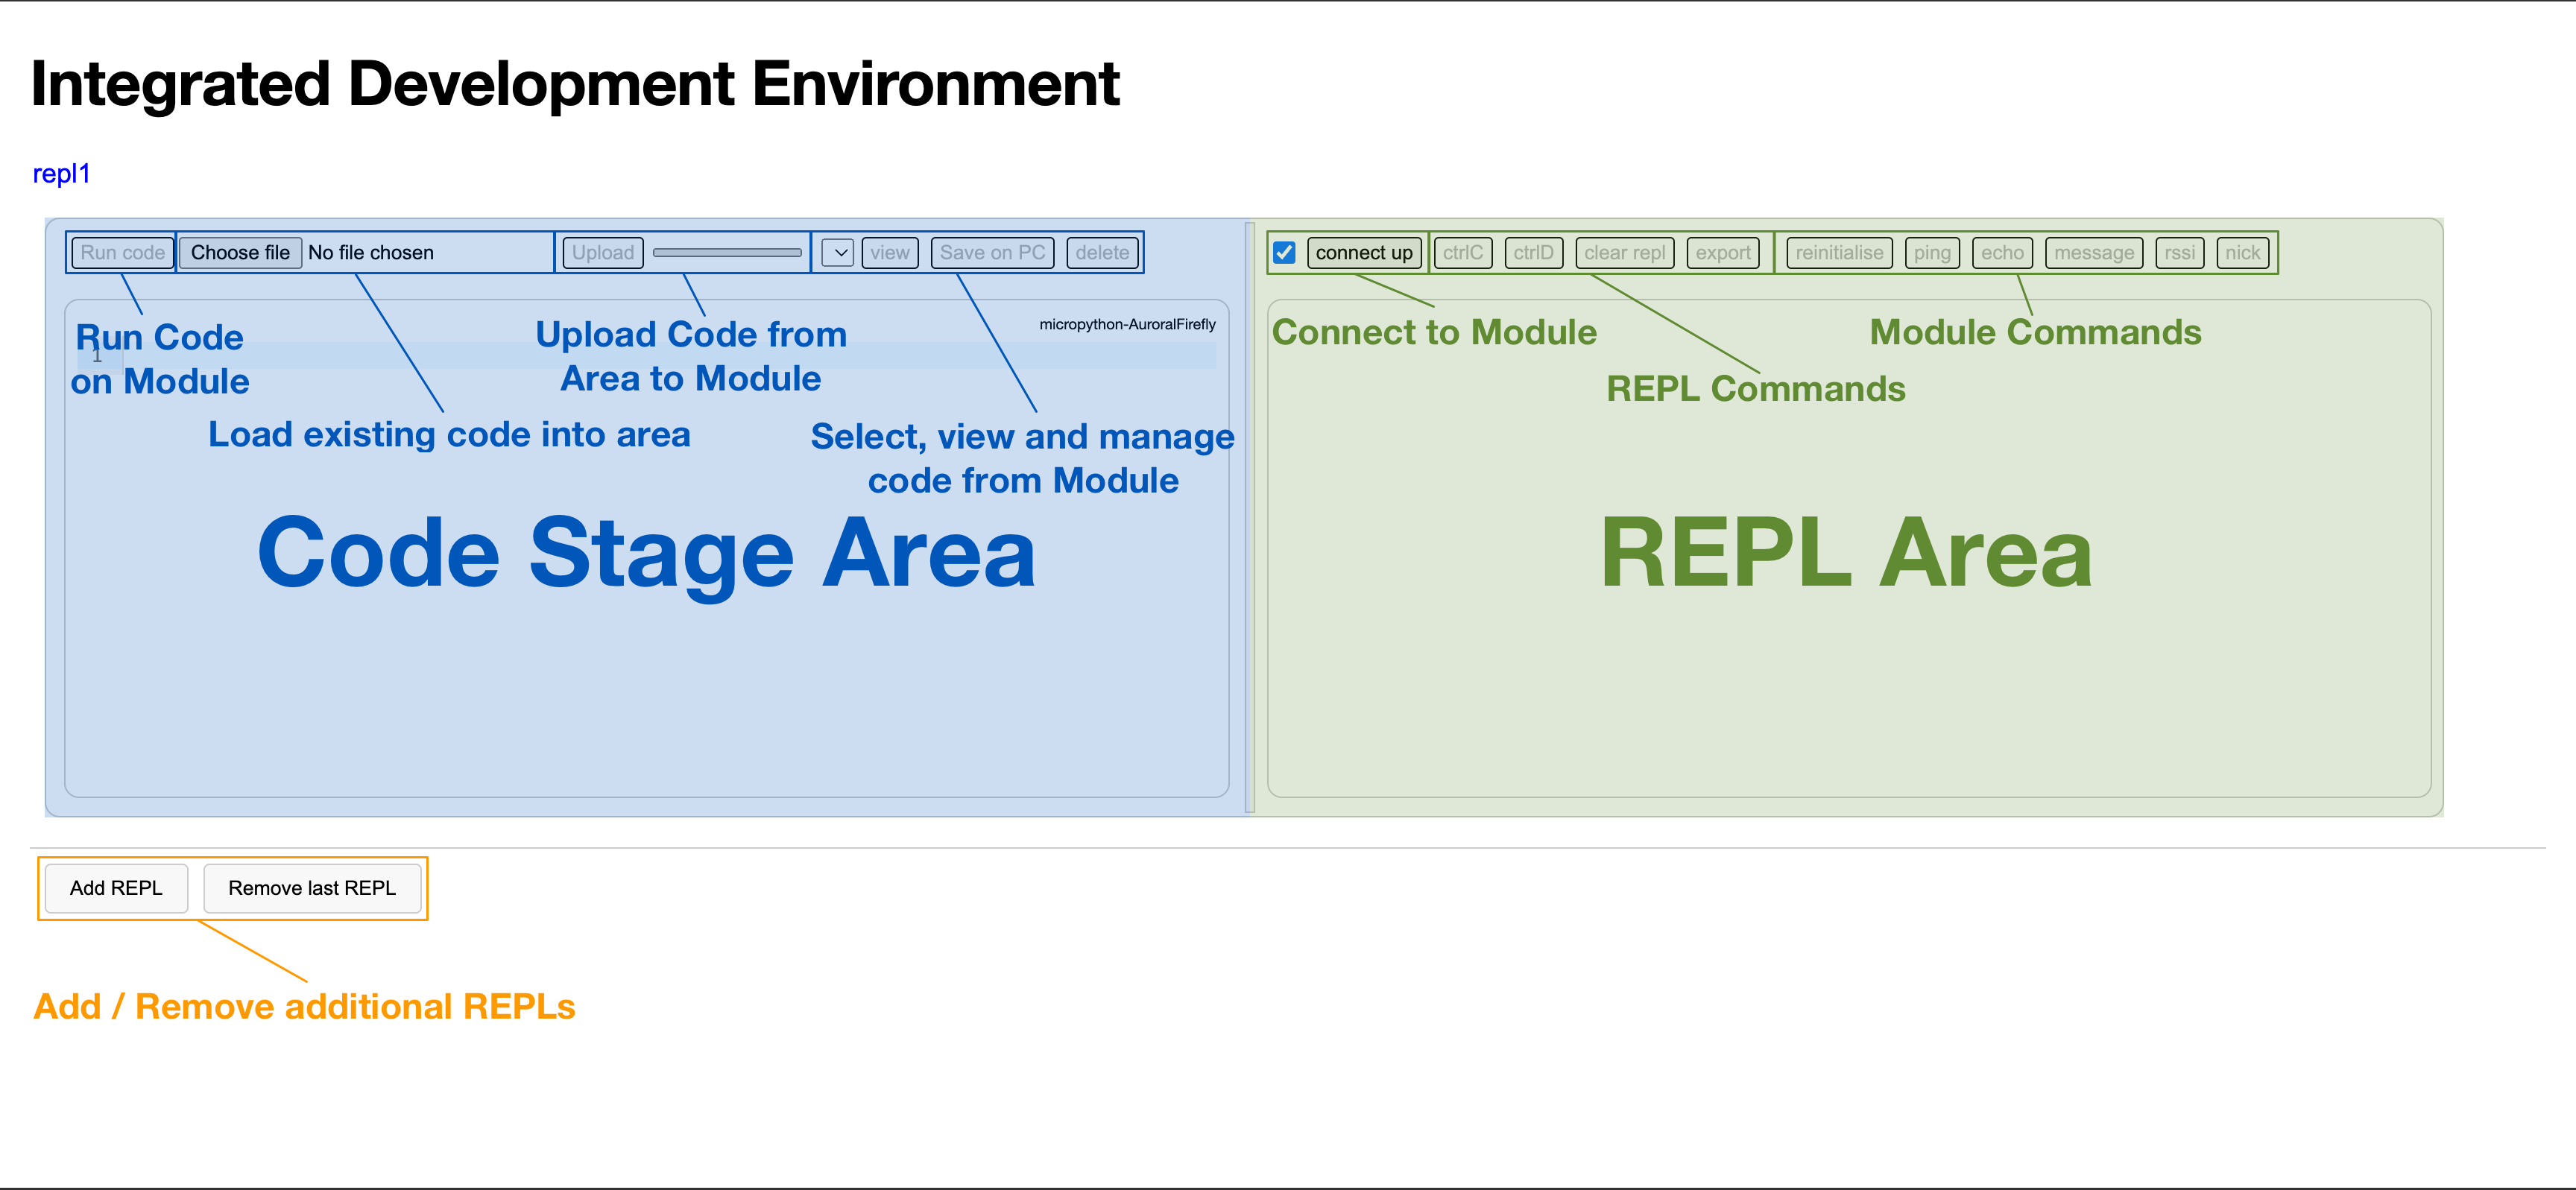
\includegraphics[width=\linewidth]{overleaf/images/ide.png}
    \vspace{\ftspace}
    \caption{IDE}
    \vspace{\ftspace}
    \label{fig:ide}
\end{figure}

Terminal pages can be added and removed using the Add REPL and Remove last REPL buttons. This allows multiple terminal pages to be added, which has been done in an effort to facilitate concurrent coding on multiple devices or modules, which is especially helpful when using the networking library. This capability comes directly from a shortcoming in other IDEs. For example, Thonny, a beginner-friendly Python IDE \citep{annamaa_thonny_2015, aivar_annamaa_thonny_2025,aivar_annamaa_thonny_nodate, annamaa_introducing_2015}, only allows one window to be open at a time.\\

\textbf{\label{sec:methods_configai}AI Code Assistant}\\\\
In an effort to ease the learning curve and simplify development of code using the Networking Library and other SSP libraries, a Large Language Model (LLM), specifically  OpenAI's Chat-GPT, has been primed with instructions, coding documentation and documented code examples.

\textbf{\label{sec:methods_nmt}Network Management and Module Configuration Tool}\\\\
To be able to manage the network and all the modules in the vicinity, the Network Management and Module Configuration Tool has been developed using PyScript based on the SSP IDE.

The concept of the Network Management and Module Configuration Tool is shown in Figure \ref{fig:nmmct_concept}. The website uses information provided by the REPL to populate a list of modules and their information. It also introduces several commands that allow commands and messages to be sent to the selected modules from the Admin module. The website simply creates the commands based on the module information and, if applicable, user-provided content, and sends the command to the REPL, where it is received and executed by the Admin Module.

\begin{figure}[H]
    \centering
    
\includegraphics[width=0.5\linewidth]{overleaf/images/placeholder.png}
    \vspace{\ftspace}
    \caption{Functionality concept of the Network Management and Module Configuration Tool}
    \vspace{\ftspace}
    \label{fig:nmmct_concept}
\end{figure}

As shown in Figure \ref{fig:nmmct}, the page is divided into three parts, the bottom part is the code stage area, the middle part contains the REPL area of the associated admin module, while the top part hosts the module management area. 
The code stage area and the REPL area are almost identical in functionality to the corresponding areas of the IDE. 
The module management area, as the name suggests, is the area where all the modules that have been in contact with the admin module, i.e. are in the vicinity of the admin module and have responded to a ping message, are listed and can be managed directly from the list using various networking commands sent from the admin module to the respective modules. The module management area consists of several parts, the list of modules with their information, such as the status of the module, its name, its MAC address, its chip ID, its configuration, its code version, the time since the last ping and the last message received, as well as the RSSI value of the last transmission from the respective device as received by the Admin Module, and some specific commands to be sent to this module (boop, ping, reboot), a list header with the information titles, and additional commands to be sent to all modules selected by the checkbox, such as the name change command, the hive set command, which puts a device in hive mode and allows it to use its hive configuration to interact with other modules, and the set hive configuration commands, which set the hive configuration of a specific module. The panel also contains a panel header which provides controls for the panel, such as a refresh button which retrieves the latest information from the Admin module, an auto-refresh select button and a debug message box.

\begin{figure}[H]
    \centering
    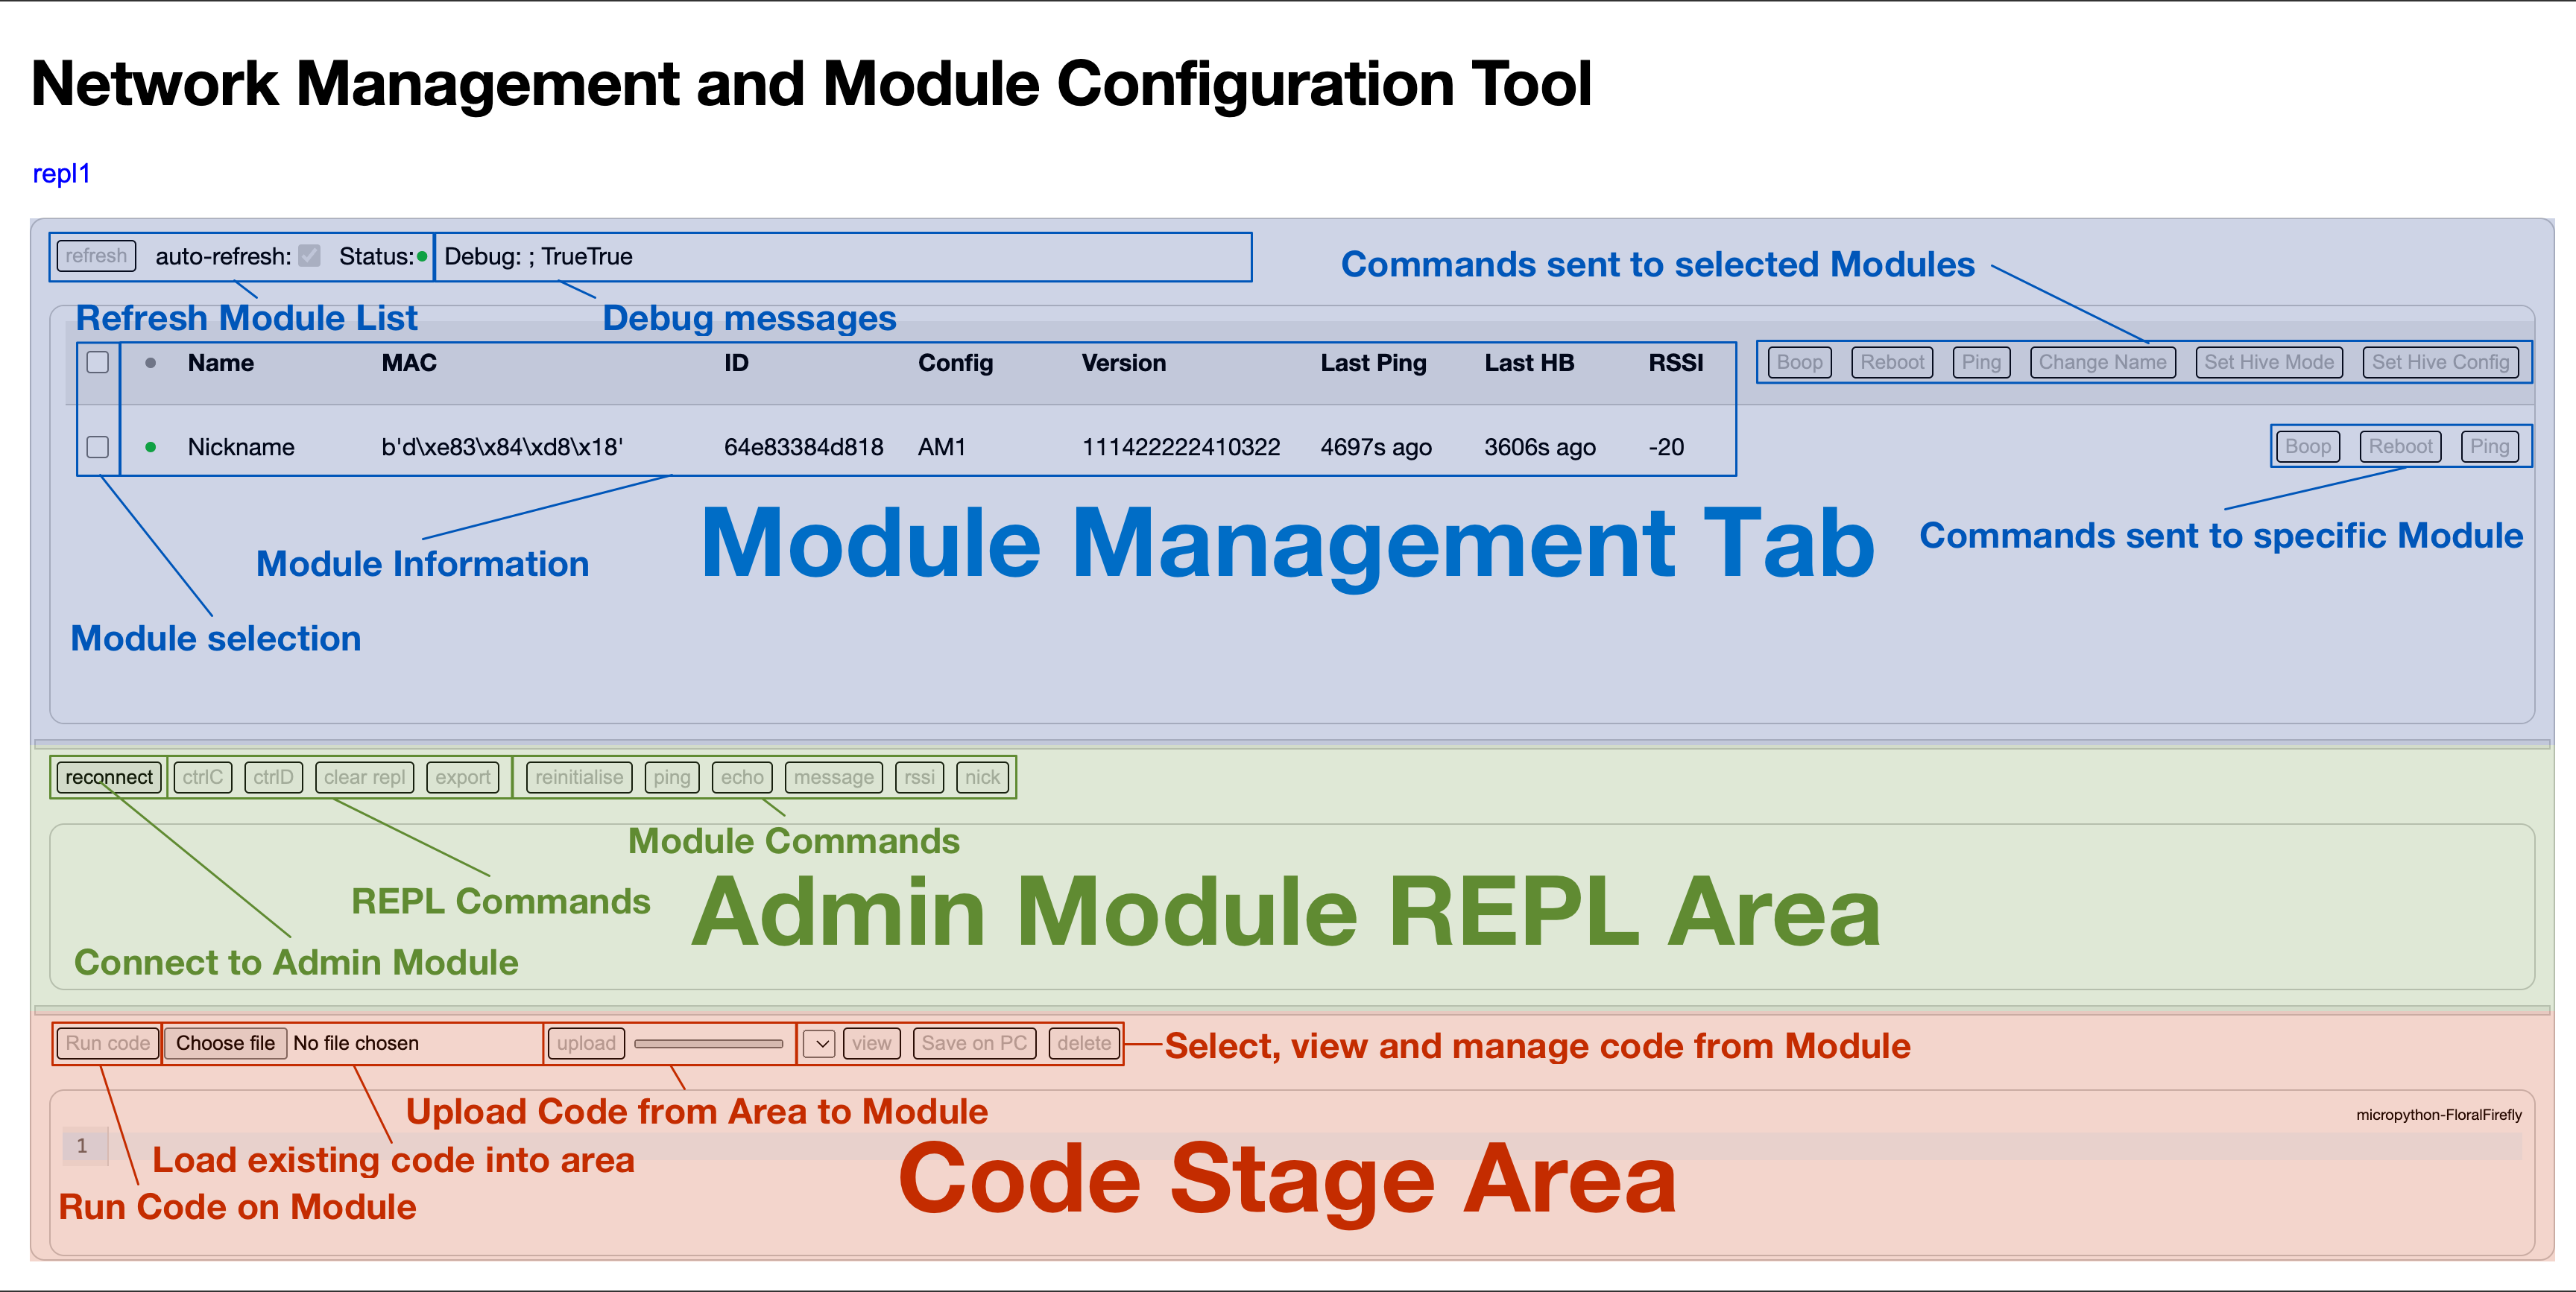
\includegraphics[width=\linewidth]{overleaf/images/nmmct.png}
    \vspace{\ftspace}
    \caption{Network Management and Module Configuration Tool}
    \vspace{\ftspace}
    \label{fig:nmmct}
\end{figure}

\textbf{\label{sec:methods_codeai}AI Module Configuration Assistant}\\\\
In an effort to simplify the configuration of Smart Modules using the Set Hive Config command of the Network Management and Module Configuration Tool, another LLM, again using OpenAI's Chat-GPT, has been primed with documentation and instructions to take a description of the available modules, as well as the required interaction configuration, and return the respective values to be provided when sending the configuration command.\\

\textbf{\label{sec:methods_up}Module Management Portal}\\\\
To update the code files on a given module, the module page has been developed using PyScript, which checks the config.py file for version numbers against the latest config.py file on the release branch of the GitHub page. If a mismatch is detected, the appropriate files are downloaded from GitHub to the webpage, which writes the files to the module, updating the software files on the device to the latest version based on its specific configuration.\\

\subsubsection{\label{sec:methods_website}Website}
In addition to the GitHub, and to better provide an overview and introduction to the concept of the Smart System Platform and its networking capabilities, host guides, documentation, as well as the developed management and development tools and contact information, a website was created.\\

For simplicity sake, the he website is hosted as part of the GitHub repository, which allows one website to be hosted and comes with an automatic release pipeline for the website whenever a change is made to the underlying files in the docs folder.

To keep in line with the designing principles of keeping things simple, accessibility and with the main goal of conversation of information and outreach in mind, the minimalistic Swiss design style was chosen to convey the information in a clear and functional fashion, using a grid system, with function dictating form \citep{muller-brockmann_grid_2020, hollis_swiss_2006}. Both a version for desktop and mobile devices was developed, with the design draft of various elements of both being shown in Figure \ref{fig:website_layout}.

\begin{figure}[H]
    \centering
    \begin{subfigure}{.18\textwidth}
        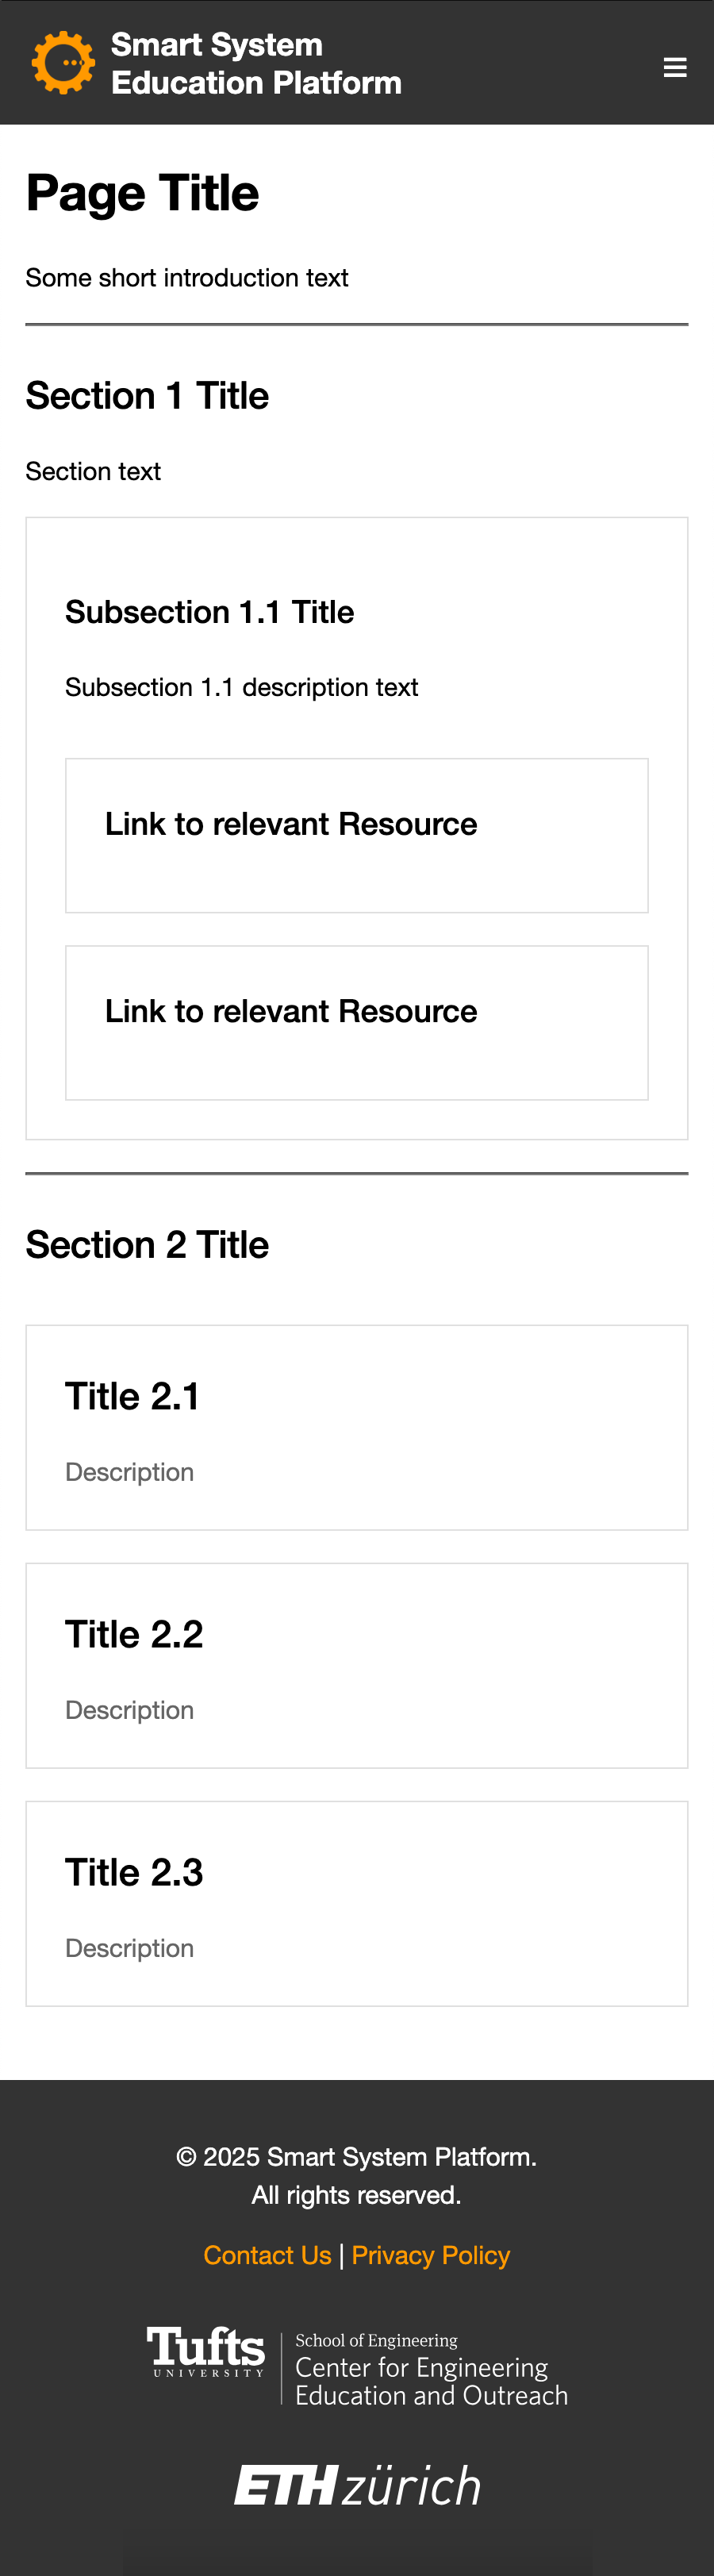
\includegraphics[height=310pt]{overleaf/images/website_mobile.png}
        \caption{Mobile version}
    \end{subfigure}
    \begin{subfigure}{.81\textwidth}
        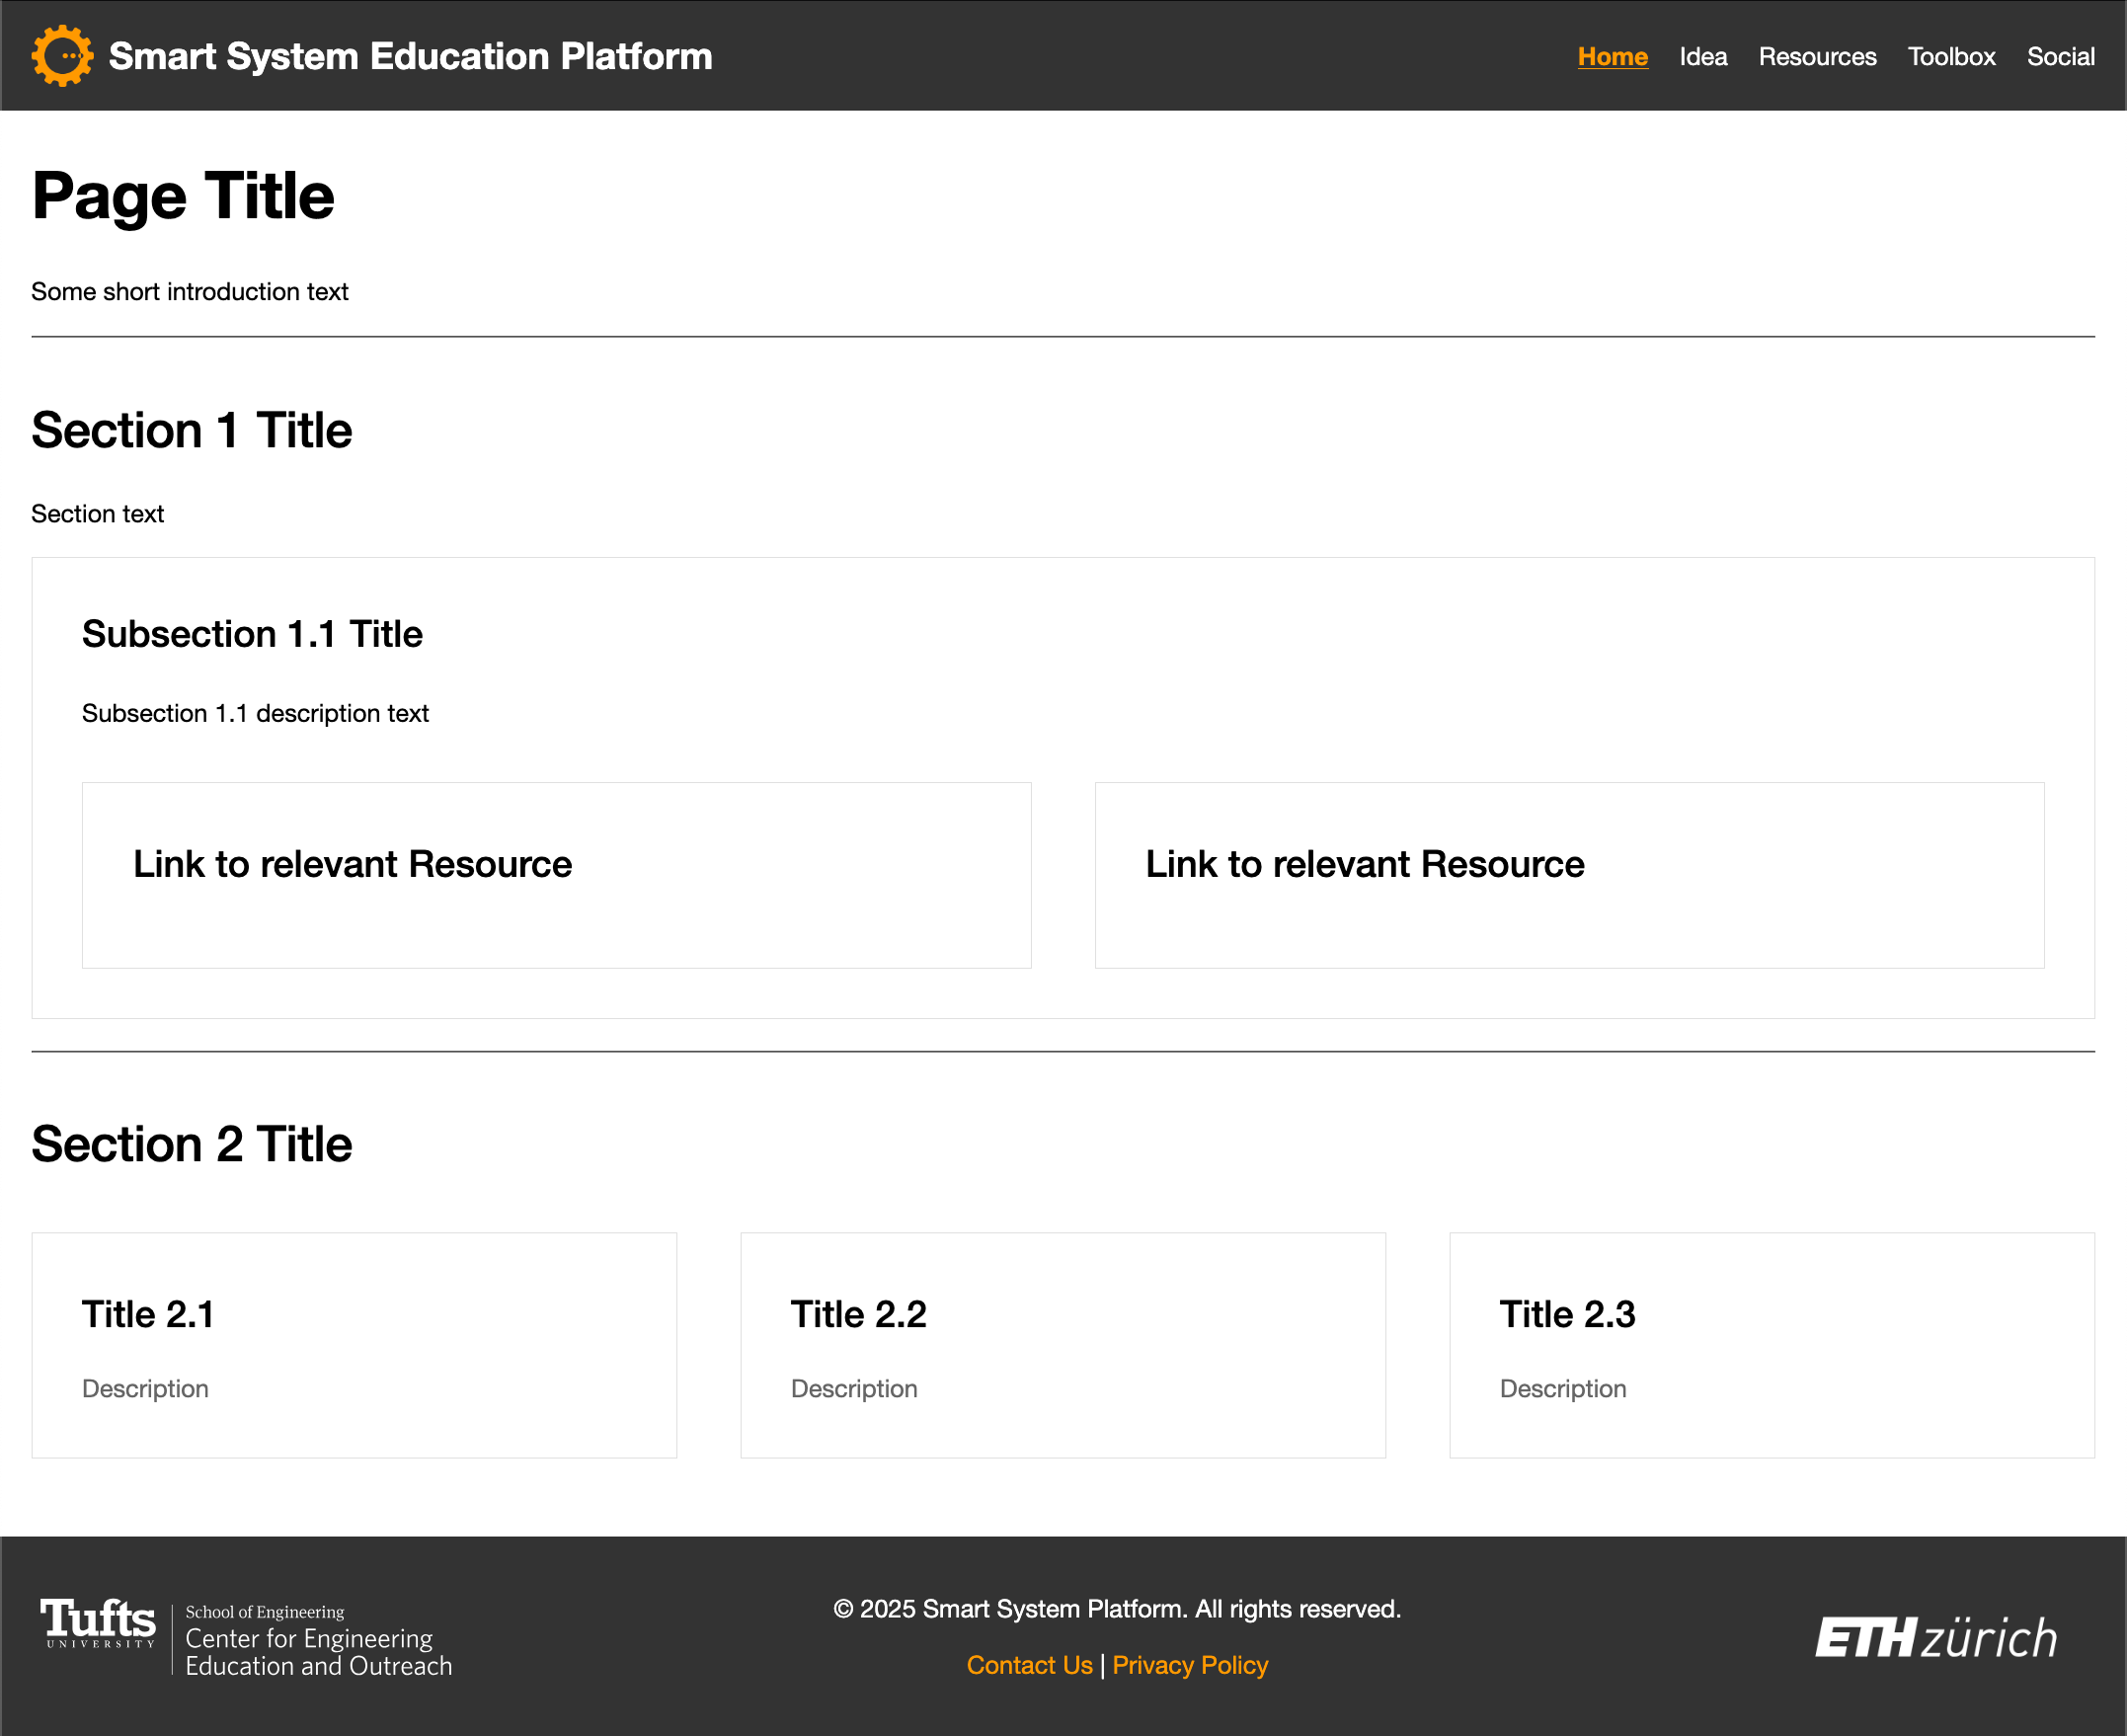
\includegraphics[height=310pt]{overleaf/images/website_desktop.png}
        \caption{Desktop version}
    \end{subfigure}
    \vspace{\ftspace}
    \caption{Website layout}
    \label{fig:website_layout}
\end{figure}

The website is divided into five parts: the home page or index page, which gives a brief introduction and overview of the Smart System Platform and provides links to the main resources; the idea page, which describes the concept of the Smart System Platform, the networking approach and provides technical background; the resources page, which contains a guide to getting started with the Smart System Platform, its tools and the Networking Library and links various other resources; the toolbox page, which links to the various tools developed, such as the IDE, the Network Management portal, the Module Management portal and the primed AI chatbots; and the social page, which provides background on the involved parties and the contact details. The different pages and their contents are also outlined in the table \ref{tab:website_content}.

\begin{table}[H]
    \centering
    \begin{tabular}{|l||p{70pt}|p{70pt}|p{70pt}|p{70pt}|p{70pt}|}
        \hline
        \textbf{Page} & Index & Idea & Resources & Toolbox & Social \\\hline
        \textbf{Content} & Overview & eh & eh & eh & eh \\
    \end{tabular}
    \vspace{\ftspace}
    \caption{Website structure and page content}
    \label{tab:website_content}
\end{table}

\subsubsection{\label{sec:methods_sw}Software}

Various code and libraries have been written and collected as part of the platform, in addition to the networking library designed and developed in Section \ref{sec:methods_net_des} and Section \ref{sec:methods_net_dev} respectively. An overview of all SSP-related code and libraries, including their purpose and source where applicable, can be found in Table \ref{tab:software_files}.

The various configuration files, such as prefs.py and version.py from the Smart Motors (see Section \ref{sec:methods_sm_soft}), have been merged into config.py, which contains other configuration values necessary for the networking and normal operation of the modules, such as the module configuration, id, code version numbers, and the STA and AP Wi-Fi channel on which the devices are operating. Except for the module type and its name, the values are set automatically when the module is powered up.  The file also contains dictionaries of network type and subtype keys and their codes, network handshake keys and codes, a whitelist of MAC addresses from which certain commands are accepted, and Wi-Fi network secrets for connecting to a specific Wi-Fi. The file also contains an i2c dictionary of common peripheral hardware i2c addresses and a dictionary of sensors and their respective range of output values, as well as the hive configuration, which includes values for which MAC addresses to send sensor data to, which devices to expect data from and which of their sensor values to use, how to use them, the rate at which data should be sent and output calculated, and more.

A customisable boot program has also been written, which automatically calls the appropriate module main program from within boot, based on a value in config.py. The module's main program will first initialise the network so that the module can be found and receive messages and commands, set up everything based on its configuration, and then either run in hive mode or call the module's stand-alone main program. This allows the module to function as a stand-alone, but still receive and respond to commands using the networking library if necessary. These commands can be used to change its configuration and, for example, put it into hive mode. To enable certain hardware inputs and outputs, such as sensors, motors, lights, etc., various libraries are also required to support their functions, which are also included in the code list.

\begin{table}[H]
    \centering
    \begin{tabular}{|l|p{180pt}|l|}
        \hline
        \textbf{File} & \textbf{Purpose} & \textbf{Credit} \\
        \hline\hline
        config.py & Configuration File & \citet{triebold_smart_2025} \\
        \hline
        boot.py & Loads main program based on module configuration & \citet{triebold_smart_2025} \\
        \hline
        main.py & Empty &  \\
        \hline\hline
        am1.py & Admin Module main code & \citet{triebold_smart_2025} \\
        \hline
        hm3.py & Hive Motor main code & \citet{triebold_smart_2025} \\
        \hline
        sl1.py & Smart Light main code & \citet[]{dahal_smart_2025} \\
        \hline
        sm3.py & Smart Motor main code & \citet[]{dahal_smart_2025} \\
        \hline
        sp1.py & Splat Module main code & \citet{triebold_smart_2025} \\
        \hline\hline
        networking.py & Library to enable ESP-NOW based networking for modules & \citet{triebold_smart_2025} \\
        \hline
        ssp\_networking.py & Library with SSP-specific networking add-ons and custom cmd types and handlers & \citet{triebold_smart_2025} \\
        \hline\hline
        adxl345.py & Library to support the built in accelerometer & \citet[]{nanawangdfr_micropython_nodate}\\
        \hline
        files.py & Library to simplify file saving and reading for Smart Motor & \citet[]{dahal_smart_2025} \\
        \hline
        icons.py & Library with icons for the screen of the Smart Motor & \citet[]{dahal_designing_2024} \\
        \hline
        sensors.py & Library to support sensors of the Smart Motor and Dahal Board & \citet[]{dahal_smart_2025} \\
        \hline
        servo.py & Library to support servo of the Smart Motor & \citet[]{dahal_smart_2025} \\
        \hline
        smartlight.py & Library to support the LED light ring of the Smart Light & \citet[]{dahal_smart_2025} \\
        \hline
        splat.py & Library to support the components of the Splat module & \citet{hankin_smart_nodate} \\
        \hline
        ssd1306.py & Support for the built in OLED screen & \citet{lehmann_micropython_nodate} \\
        \hline
        variableLED.py & Library that powers the variable LED grid & \citet{hankin_smart_nodate} \\
        \hline
    \end{tabular}
    \vspace{\ftspace}
    \caption{Overview of all the software files, including libraries and their purpose}
    \label{tab:software_files}
\end{table}

\subsubsection{\label{sec:methods_hw}Hardware}
%Modules, overview of existing technology, go into the analysis results of the used software, firmware and chips, how modular they are and what could be used for them and show the graphics with example input / output matrix as 
During the development of the Networking Library and the Smart System Platform, in terms of hardware, Smart Motors were used, alongside other prototyped derivatives such as the Smart Light, which is a Smart Motor which uses an LED ring instead of a motor as output, and stand-alone Dahal Boards, as well as certain prototypes from the Smart Playground project such as the Splat Module and the Button Module. The Dahal Board especially, proved to be a useful asset, thanks to its many interfaces, outlined in Section \ref{fig:sm_dahal_board}, allowing plug and play with a variety of sensor inputs and outputs. An overview of the possibilities, based on which any Smart Modules could be developed, can be seen in Figure \ref{fig:met_hardware}.

\begin{figure}[H]
    \centering
    \includegraphics[width=.75\linewidth]{overleaf/images/Smart Systems Platform-io.drawio.png}
    \vspace{\ftspace}
    \caption{Hardware matrix with possible inputs and outputs for Smart Modules}
    \label{fig:met_hardware}
\end{figure}

As part of the ongoing Smart Playground project \citep{jess_smart_2025}, which will be further introduced in Section \ref{sec:methods_smart_playground}, certain modules have been developed that are consistent and compatible with the Smart System Platform approach, in particular using the developed Networking Library, the use of which is described in section \ref{sec:res_smartplayground}.The hardware developed for the Smart Playground project, shown in figure \ref{fig:hardware_examples}, includes a Button Module and a Splat Module, based on the Splat toy, but both using an ESP32C6 MCB (see Figure \ref{fig:esp32c6}), as well as Plushies and , based on the Dahal board, using an ESP32C3 MCB (see Figure \ref{fig:esp32c3}), both introduced in Section \ref{sec:rev_esp}.

\begin{figure}[H]
    \centering
    \begin{subfigure}[b]{0.25\textwidth}
        
\includegraphics[width=\linewidth]{overleaf/images/placeholder.png}
    \end{subfigure}
    \hspace{10pt}
    \begin{subfigure}[b]{0.25\textwidth}
        
\includegraphics[width=\linewidth]{overleaf/images/placeholder.png}
    \end{subfigure}
    \hspace{10pt}
    \begin{subfigure}[b]{0.25\textwidth}
        
\includegraphics[width=\linewidth]{overleaf/images/placeholder.png}
    \end{subfigure}
    \\
    \begin{subfigure}[b]{0.25\textwidth}
        
\includegraphics[width=\linewidth]{overleaf/images/placeholder.png}
    \end{subfigure}
    \hspace{10pt}
    \begin{subfigure}[b]{0.25\textwidth}
        
\includegraphics[width=\linewidth]{overleaf/images/placeholder.png}
    \end{subfigure}
    \hspace{10pt}
    \begin{subfigure}[b]{0.25\textwidth}
        
\includegraphics[width=\linewidth]{overleaf/images/placeholder.png}
    \end{subfigure}
    \\\vspace{\ftspace}
    \caption{Smart Light Module (left), Splat Module (middle) and Button Module (right), Smart Boards () and Plushies () \citep{jess_smart_2025}}
    \label{fig:hardware_examples}
\end{figure}

\subsubsection{\label{sec:methods_fw}Firmware}
While a custom firmware was built for the Smart Motors with additional packages and libraries, and it was briefly considered to do the same and create our own firmware and include certain libraries, especially the networking library, in the firmware, it was decided not to do this, but to use the base MicroPython firmware for the sake of accessibility and interoperability.

\section{\label{sec:methods_ph3}Phase 3: Testing and Validation}
In a final phase, the developed Networking Library was tested and an attempt was made to test and validate the various parts, such as the tools and capabilities developed for the Smart System Platform.

\subsection{\label{sec:methods_test_net}Networking}
The following tests were designed during the development of the Networking Library to assess, test and validate its networking capabilities.

\subsubsection{\label{sec:methods_test_boop}Robustness - Boop-o-Meter}
In an effort to assess and test the reliability and sturdiness of the Networking Library with a larger amount of modules, a program called the boop-o-meter\footnote{The name is a reference to he Tumblr April 1st joke in 2021, by which the tool was inspired} was created. The program runs on Dahal-Board hardware and uses a simple interaction design, discovering all modules in its vicinity using the ping functionality of the Networking Library, and then lists all the discovered modules in a list on the screen and then allows a message to be sent to the highlighted mac address in a list of mac addresses of discovered devices, which also includes the broadcast address, keeping count of received and sent messages. The test was conducted during Hackathon 1 with 18 devices, the goal was then to send and receive 999 messages.

% \begin{figure}[H]
%     \centering
%     \includegraphics[width=\linewidth]{overleaf/images/Smart Systems Platform-io.drawio.png}
%     \vspace{\ftspace}
%     \caption{Boop-o-meter UI design}
%     \label{fig:boop-o-meter}
% \end{figure}

The results of this test are outlined in Section \ref{sec:res_reliability} and the code can be found in Appendix \ref{chap:apx_e}.

\subsubsection{\label{sec:methods_test_range}Range}
A further test was carried out to determine the maximum range at which messages could still be received, using the same programme as described for the robustness test, the code for which can be found in Appendix \ref{chap:apx_e}. Given the range requirements for this test, the test was conducted outdoors on a straight road between the CEEO offices and the Tufts campus to ensure an uninterrupted line of sight. 
Two people, connected via phone call, walked away from each other on the street and periodically sent messages to each other from the MCB. At the point where neither person was receiving messages, their positions were marked and the final distance was calculated using Google Earth. The results of this test are discussed in Section \ref{sec:res_range}.

\subsubsection{\label{sec:methods_test_rssi}Response Time, RSSI and Packet Loss Rate by Range}
To test the reliability of the transmission and to get an idea of the response time, RSSI values and packet loss by range, a test was carried out at different distances. As this code was intended to demonstrate the technical capabilities of the underlying ESP-NOW protocol, a specific code was written for this test, reducing the code and networking part to the absolute minimum. The code was designed to send 100 messages to the broadcast address, with the receiving module designed to echo the messages immediately on receipt. Sending was triggered manually and message exchange was monitored with print statements. The various modules logged relevant data, such as the message ID (to calculate the number of dropped messages), the time of reception and transmission to calculate the ping of a message sent back and forth, and the RSSI value. In a separate step, the logged raw values were then written to a file, and the various values of interest were calculated and stored in a separate step at the end. The code was kept to a minimum and the logged data was written after the fact to allow sufficient time for all messages to be received and returned. The test was carried out in two stages: for distances of less than one metre, the test was carried out in the laboratory, while for longer distances, in order to ensure a clear line of sight between the two devices, given the distance requirements, the test was carried out outdoors on the roof of the car park outside the CEEO offices at 200 Boston Avenue, MA, USA. The results of this test are discussed in Section \ref{sec:res_rssi} and the corresponding code and raw results can be found in Appendix \ref{chap:apx_e}.\\\\
A further response time test was conducted using the Networking Library, to measure the time taken up by the additional calculation burden imposed by the library, which is discussed in Section \ref{sec:res_ping}.
%(Temperatures for the outised tests were at -4* celsius with clear weather and some wind gusts.)

\subsubsection{\label{sec:methods_test_angle}Antenna Angle Effects on RSSI and Ping}
Based on anecdotal observations from the Smart Playground project using ESP32C3 and ESP32C6 devices with the developed SSP Networking Library, differences in RSSI values, which were used to approximate range, were observed for different devices. The effect of the relative antenna angle between two units was tested at a predefined distance of 1 metre, as outlined in Figure \ref{fig:angle}. The same program used to calculate the response time, RSSI values and packet loss rate for different distances was used for this test, the code for which can be found in Appendix \ref{chap:apx_e}. The results of this test are presented in Section \ref{sec:res_angle}.

\begin{figure}[H]
    \centering
    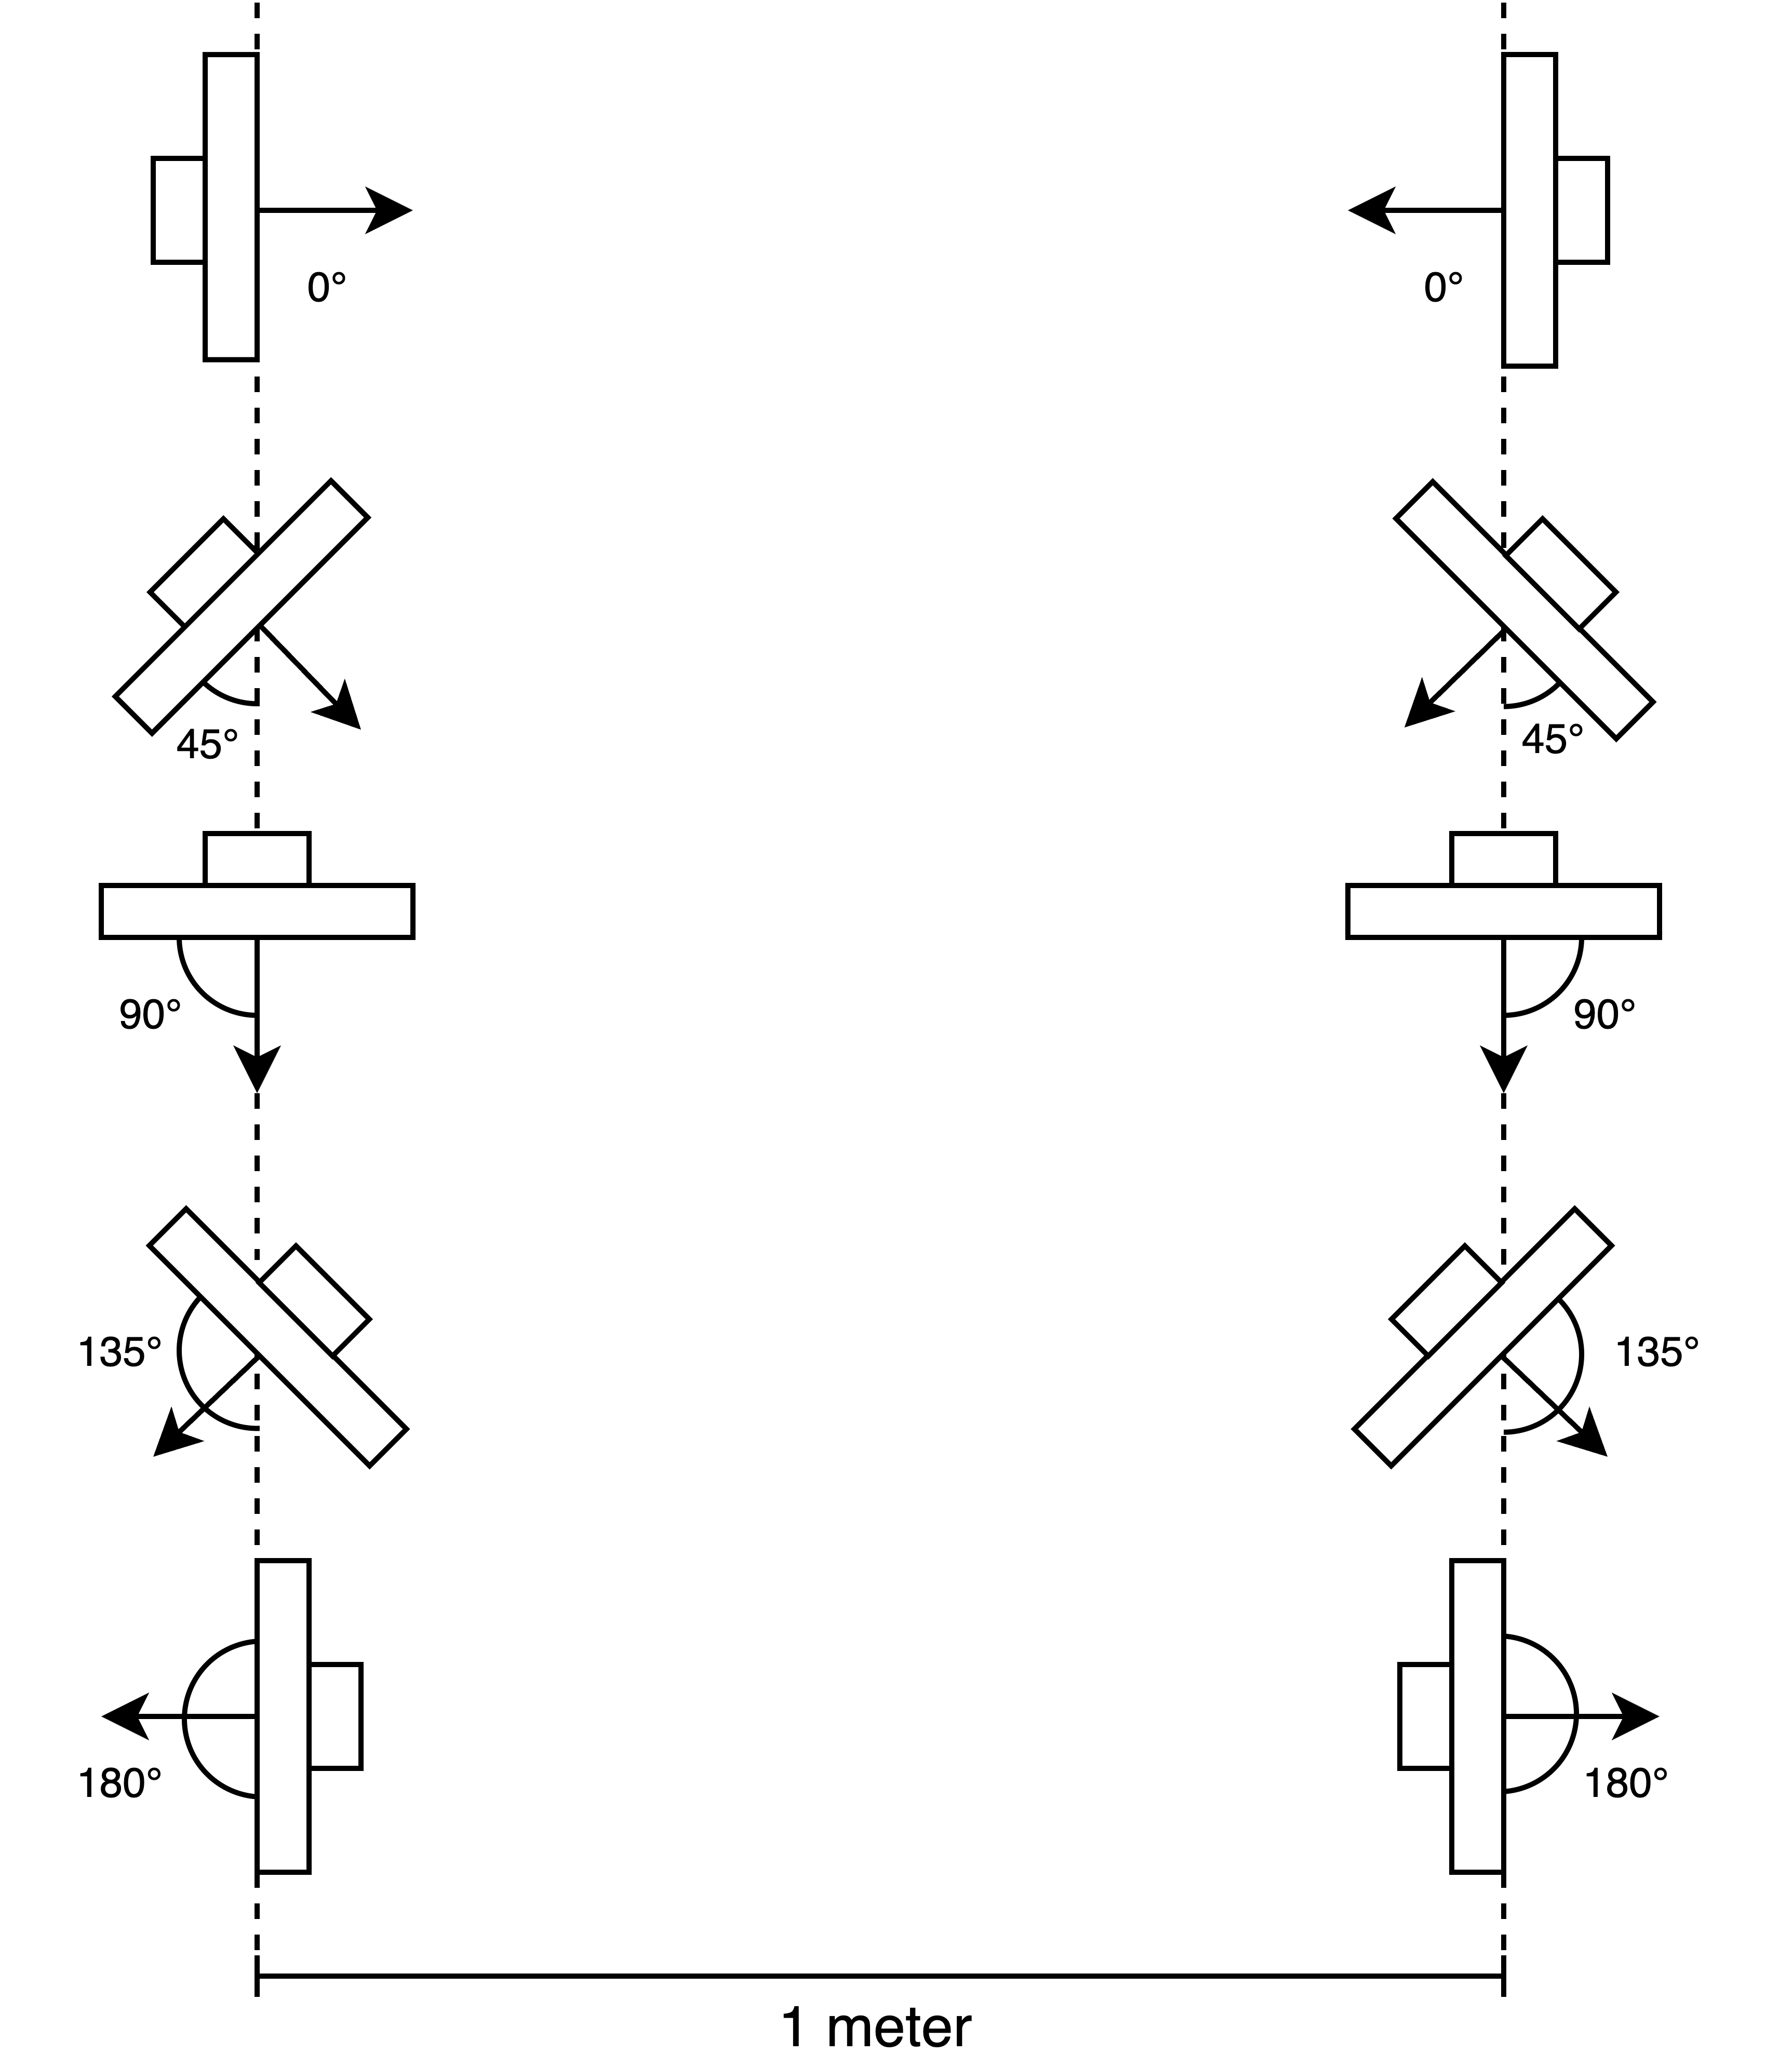
\includegraphics[width=0.5\linewidth]{overleaf/images/angletest.drawio.png}
    \vspace{\ftspace}
    \caption{The various setups to test antenna angle effects on response time, RSSI and packet loss rate}
    \label{fig:angle}
\end{figure}

\subsubsection{\label{sec:methods_test_batter}Power Consumption}
Another test that was prepared after problems were discovered by the Smart Playground project when using networking in conjunction with various additional components such as audio output and LED lights, powered by three AAA batteries instead of the usual LiPo batteries, was that after about ten minutes the power was too low to run all three components simultaneously. To this end, a test was designed and carried out to determine the power consumption of the Networking Library when continuously sending and receiving messages. Starting with a full LiPo battery, echo type messages were sent every second, while a receiver connected to a laptop continued to log the time since startup when the last message was received. The code for this test can be found in Appendix \ref{chap:apx_e}, while the results are outlined in Section \ref{sec:res_battery}.

\subsection{\label{sec:methods_tools}Smart System Platform: GitHub, Tools and Website}

While it was possible to conduct an accessibility and design test for the website, using the Google Developer's PageSpeedInsights \citep{noauthor_about_nodate}, validation of the Smart System Platform as a whole, the GitHub, the website and the tools and the code and networking libraries can only be achieved by continued use, as described in and Section \ref{sec:methods_other}. However, an attempt to test it was made during the two Hackathons, outlined in Section \ref{sec:methods_hackathon1} and Section \ref{sec:methods_hackathon2}.

\subsubsection{\label{sec:methods_example}Example Applications}
Some example applications were developed by the author during the research, using the developed Networking Library and Smart System Platform and its tools, such as the boop-o-meter, Smart Motors controlling each other and the Hive Motors project, which describes the Smart Modules set up to be configurable using the Network Management and Module Configuration Tool. The results of this are described in Section \ref{sec:res_examplekit}.

\subsection{\label{sec:methods_hackathon1}Hackathon 1}

The focus of the first hackathon was to test the robustness of the Networking Library and ESP-NOW and to explore the use and usability of the Networking Library. The hackathon was therefore divided into several parts, starting with an introduction to the research, the Networking Library and the proposed Smart System Platform. This was followed by a robustness test using the boop-o-meter program, as described in Section \ref{sec:methods_test_boop}. As a next step, the participants were tasked with brainstorming potential uses and applications of such a networked device, and then using the provided networking library and example code to build a small project using Smart Motors hardware. The results are outlined in Section \ref{sec:res_hackathon1}.

\subsection{\label{sec:methods_hackathon2}Hackathon 2}

The focus of the second hackathon was to test the Smart System Platform as a whole, focusing on the usability of the development tools and the Networking Library, and to find out what students could do with the tools and capabilities provided. The hackathon will start with an introductory presentation about the project, the Networking Library and the Smart System Platform approach, a quick overview of the tools. Participants are then tasked in small groups to try out the tools and develop a small interactive project using the Networking Library and Smart System Platform tools. Feedback on the usability as well as the application potential was collected via a questionnaire, the results of which are discussed in Section \ref{sec:res_hackathon2}.

\subsection{\label{sec:methods_other}Use in Other Projects}

\subsubsection{\label{sec:methods_me35}ME35}
Some students have used the GitHub and Networking Library for some of their class projects as part of the Tufts class ME35, whose feedback was also gathered via questionnaire. The results of this, as well as the project developed using the provided networking capability are shown in Section \ref{sec:res_me35}.

\subsubsection{\label{sec:methods_smart_playground}Smart Playground}
%Introduce project and that code and some of the ideas outlined in Section \ref{sec:methods_ssp_des} and Section \ref{sec:methods_ssp_dev} were used for this project.
The Smart Playground project, developed concurrently with this research as a partnership between Tufts CEEO and Boston University, is a project... introduce project. 
The main goal of the project is to create interactive playground and classroom experiences to teach computational thinking. The approach taken was to use interactive modules, some of which are carried or held individually by children, and others in the form of stations such as buttons or splats (see Section \ref{sec:methods_hw}). As such, the project required a way for the different modules to communicate and interact with each other, which was exactly the capability developed as part of this research in the form of the Networking Library. The project also based its hardware on the Dahal Board and ESP32 MCBs, which are fully compatible and in line with the aims of the Smart System Platform, one of which is to enable and facilitate such development, leading to some collaboration. The project relied on the Networking Library to develop the hardware for its initial tests, and used some of the ideas outlined in Section \ref{sec:methods_ssp_des} and Section \ref{sec:methods_ssp_dev} to develop hardware that is compatible and in line with the idea of the idea of Smart System Platform introduced in Section \ref{sec:methods_ssp_des}. The use of the Networking Library by the Smart Playground project is further explored and discussed in Section \ref{sec:res_smartplayground}.



